\documentclass{apuntes}
\usepackage{tikz}
\usepackage{tikz-3dplot}
\usepackage{pgfplots}

\title{Análisis Matemático}
\author{Víctor de Juan y Guillermo Julián}
\date{13/14 C1}
\usetikzlibrary{arrows,calc,shapes}

\begin{document}

% Macros para la proyección estereográfica
\usetikzlibrary{calc,fadings,decorations.pathreplacing}
%% helper macros

\newcommand\pgfmathsinandcos[3]{%
  \pgfmathsetmacro#1{sin(#3)}%
  \pgfmathsetmacro#2{cos(#3)}%
}
\newcommand\LongitudePlane[3][current plane]{%
  \pgfmathsinandcos\sinEl\cosEl{#2} % elevation
  \pgfmathsinandcos\sint\cost{#3} % azimuth
  \tikzset{#1/.estyle={cm={\cost,\sint*\sinEl,0,\cosEl,(0,0)}}}
}
\newcommand\LatitudePlane[3][current plane]{%
  \pgfmathsinandcos\sinEl\cosEl{#2} % elevation
  \pgfmathsinandcos\sint\cost{#3} % latitude
  \pgfmathsetmacro\yshift{\cosEl*\sint}
  \tikzset{#1/.estyle={cm={\cost,0,0,\cost*\sinEl,(0,\yshift)}}} %
}
\newcommand\DrawLongitudeCircle[2][1]{
  \LongitudePlane{\angEl}{#2}
  \tikzset{current plane/.prefix style={scale=#1}}
   % angle of "visibility"
  \pgfmathsetmacro\angVis{atan(sin(#2)*cos(\angEl)/sin(\angEl))} %
  \draw[current plane] (\angVis:1) arc (\angVis:\angVis+180:1);
  \draw[current plane,dashed] (\angVis-180:1) arc (\angVis-180:\angVis:1);
}
\newcommand\DrawLatitudeCircle[2][1]{
  \LatitudePlane{\angEl}{#2}
  \tikzset{current plane/.prefix style={scale=#1}}
  \pgfmathsetmacro\sinVis{sin(#2)/cos(#2)*sin(\angEl)/cos(\angEl)}
  % angle of "visibility"
  \pgfmathsetmacro\angVis{asin(min(1,max(\sinVis,-1)))}
  \draw[current plane] (\angVis:1) arc (\angVis:-\angVis-180:1);
  \draw[current plane,dashed] (180-\angVis:1) arc (180-\angVis:\angVis:1);
}

%% document-wide tikz options and styles

\tikzset{%
  >=latex, % option for nice arrows
  inner sep=0pt,%
  outer sep=2pt,%
  mark coordinate/.style={inner sep=0pt,outer sep=0pt,minimum size=3pt,
    fill=black,circle}%
}

\pagestyle{plain}
\maketitle
\newpage
\tableofcontents
\newpage

\input{tex/0-Preliminares.tex}
\section{Diferenciación}

\begin{defn}[Función\IS diferenciable]
 $F$ es diferenciable en $\gor{a}$ si existe una aplicación lineal $L$ tal que
 
\[ \frac{F(\gx)-F(\ga)-L(\gx-\ga)}{||\gx-\ga||} \convs[][\gx][\ga] 0 \]

que se puede expresar como
\[ \lim_{\gor{h} \rightarrow \gor{0}} \frac{\md{F(\ga+\gor{h}) - F(\ga) - L\gor{h}}}{||\gor{h}||} = 0 \]
\end{defn}

\begin{defn}[Diferencial]
A esa matrix $L$ la vamos a llamar la diferencial de $F$ en $\ga$:

\[ L\equiv DF(\ga) \]
\end{defn}

\begin{theorem} 
$$F \text{ diferenciable en } \ga \implies F \text{ continua en } \ga$$
\end{theorem}

\begin{proof}
 $$\lim_{\gor{h} \rightarrow \gor{0}} \frac{\md{F(\ga+\gor{h}) - F(\ga) - L\gor{h}}}{\md{\gor{h}}} = 0$$
 Esta es la definición de diferenciable. Para que este límite sea 0, el numerador tiene que tender a 0, por lo que $F(\ga+\gor{h}) - F(\ga) \rightarrow 0$
\end{proof}


\begin{theorem} 
Si la diferencial existe, entonces es única.
\end{theorem}

\begin{proof}  Vamos a demostrar que esa aplicación $L$ es única. Supongamos que existen $L_1,L_2$ que cumplen las condiciones.
\[0=\lim_{\gor{h} \rightarrow \gor{0}} \frac{F(\gor{a}+\gor{h}) - F(\ga)-L_1\gor{h}}{||\gor{h}||} = \lim_{\gor{h} \rightarrow \gor{0}} \frac{F(\gor{a}+\gor{h}) - F(\ga)-L_2\gor{h}}{||\gor{h}||}\].

Sumando:

\[ 0 = \lim_{\gor{h} \rightarrow \gor{0}} \frac{||F(\gor{a}+\gor{h}) - F(\ga)-L_1\gor{h}|| + ||F(\gor{a}+\gor{h}) - F(\ga) -L_2\gor{h}||}{||\gor{h}||} \]

Teniendo en cuenta que $||A-B|| = ||A+(-B)|| \leq ||A||+||B||$

\[ 0 \leq \lim_{\gor{h} \rightarrow \gor{0}} \frac{2\cdot\md{F(\ga + \gor{h}) - F(\ga)} + \md{L_1\gor{h}} + \md{L_2\gor{h}}}{\md{\gor{h}}} \]

\textit{Aquí falta completar.}
\end{proof}



\paragraph{Nomenclatura: }
Aproximación lineal $\sim$ Diferencial.

Matriz jacobiana $\sim$ Jacobiana.

\begin{defn}[Matriz\IS diferencial]
 Matriz asociada a $DF(\ga) \equiv $ Matriz de las derivadas parciales de F.
 
 $$DF(\ga) \equiv \begin{pmatrix}
                \dpa{F_1}{x_1} & \cdot & \dpa{F_1}{x_N}\\
                \vdots& \ddots & \vdots\\
                \dpa{F_N}{x_1} & \cdot & \dpa{F_N}{x_N}
                \end{pmatrix}
$$
\end{defn}

\begin{theorem}
 $F$ diferenciable en $\ga \implies \exists \deriv{F_k}{x_i}(\ga), i=1,2,...,N \y k = 1,2,...,M$
\end{theorem}

El contraejemplo para demostrar la implicación a la izquierda es el mismo que en los límites a lo largo de rectas.

$f(x,y) = \left\{ \begin{matrix}

\frac{xy^2}{x+y^2} & (x,y) = (0,0) \\ 
0 & (x,y)=(0,0)
           
          \end{matrix}\right.
$

Según las aplicaciones que tengamos, la diferencial se suele llamar de una u otra forma. Con $\appl{\delta}{\real}{\real^M}$ utilizamos notación vectorial en vez de matricial porque tendríamos una matriz columna. Por ejemplo: la velocidad (en un instante de tiempo, un punto en el espacio).

\begin{defn}[Gradiente] Sea $\appl{F}{\real^N}{\real}$, entonces definimos el vector gradiente como 

\[ \grad F(\gx) = DF(\gx) = \left(\dpa{F}{x_1}, \dpa{F}{x_2},\dotsc, \dpa{F}{x_n}\right) \]
\end{defn}


\subsection{Regla de la cadena}
\index{Regla!de la cadena}
Consideremos la composición de dos funciones de la siguiente forma:

$\appl{F}{\real^N}{\real^M}$. 

$\appl{G}{\real^M}{\real^K}$.

$\appl{H=G\circ F}{\real^N}{\real^K}$.

$ \gx \in \real^N, \gy \in \real^M$

\begin{wrapfigure}{r}{0.3\textwidth}
\begin{center}
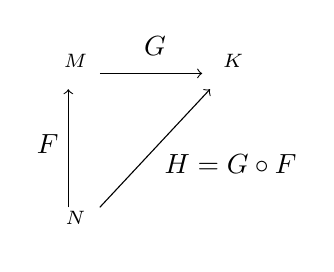
\begin{tikzpicture}
\draw[->] (-0.1,0.2) -- (-0.1,1.7);
\draw[->] (0.3,1.9) -- (1.6,1.9);
\draw[->] (0.3,0.2) -- (1.7,1.7);

\node at (0,0) {$\real^N$};
\node at (0,2) {$\real^M$};
\node at (2,2) {$\real^K$};

\node[left] at (-0.1,1) {$F$};
\node[above] at (1,2) {$G$};
\node[below right] at (1,1) {$H = G\circ F$};
\end{tikzpicture}
\end{center}
\caption{Composición de funciones}
\end{wrapfigure}

Con $F$ diferenciable en $\ga$ y $G$ diferenciable en $F(\gor{a})$. Entonces $H=G\circ F$ es diferenciable en $\ga $.
Además la expresión matricial es:

\[ \underbrace{DH(\ga)}_{K\times N} = \underbrace{DG(F(\ga))}_{K\times M}\cdot \underbrace{DF(\ga)}_{M\times N} \]
 
No hace falta calcular toda la matriz si sólo queremos un elemento. Para calcular 1 único elemento de la matriz diferencial (el de la fila $i$, columna $j$), usamos la siguiente fórmula
\[ \dpa{H_i}{x_j}(\ga) = \sum_{k=1}^M \dpa{G_i}{y_k}\cdot\dpa{F_k}{x_j} \]

Siempre teniendo en cuenta que $\displaystyle\dpa{G_i}{y_k}$ está evaluado en $F(\ga)$ y $\displaystyle\dpa{F_k}{x_j}$ está evaluado en $\ga$.

\subsection{Extensiones del Teorema del Valor Medio}

El teorema anterior que vimos del valor medio era para funciones de una variable, y proponía lo siguiente:
\begin{theorem}[Teorema\IS del valor medio (una variable)]
\label{thmTVM1var}
Dada $\appl{f}{\real}{\real}$ diferenciable, se tiene que \[ f(b)-f(a) = f'(c)(b-a)\] para algún $c\in[a,b]$
\end{theorem}

Después el teorema lo extendimos a funciones de $\real^N$ en $\real$: dada $\appl{F}{\real^N}{\real}$ entonces definíamos
 
 \[ \sigma(t)  = t\gor{b}+(1-t)\gor{a} \] 
 
 y $g = F\circ \sigma$ era una aplicación de los reales a los reales, y entonces aplicando el teorema anterior teníamos que 
 
 \[ F(\gor{b}-\gor{a}) = g(1)-g(0)  = g'(s) \] 
 para algún $s\in[0,1]$.

Sin embargo, al tratar de extrapolar este resultado a una función $\appl{F}{\real^N}{\real^2}$ nos queda que 

 \[ F(\gor{b})-F(\ga) = \begin{pmatrix}
                         \pesc{\nabla F_1(\gor{c_1}),{\gor{b}-\ga}}\\
                         \pesc{\nabla F_2(\gor{c_2}),\gor{b}-\ga}
                        \end{pmatrix}
 \]
  Tenemos 2 $c$ distintos, uno para cada $f$, por lo que este teorema pierde sentido. Hay que buscar una extensión, otra formulación del teorema que nos permita aplicarlo a las funciones que estamos estudiando.
  
  \begin{theorem} [Teorema\IS del valor medio (varias variables)]
  \label{thmTVM}
  Sea $f \in C^1$ en un abierto que contenga $[a,b]$. Entonces 
  
  \[ \norm{F(\gor{b})-F(\ga)} \leq \md{DF(\gor{c})} \cdot \md{\gor{b}-\ga} \]
  
  Siendo $c$ un punto del segmento que une $\ga$ y $\gb$ en el que $\md{DF(tb+(1-t)a)}$ alcanza su máximo.
  \end{theorem}  
  
  \begin{proof}

Primero vamos a demostrar la siguiente desigualdad:

\begin{equation}
\label{eqnTVM1}
 \md{\int_0^1 F(t) \,dt}≤ \int_0^1 \md{F(t)}\,dt 
\end{equation}

Si tomamos \[ L = \int_0^1 F(t) \,dt \]  entonces

\[ \md{L}^2 = \md{\int_0^1 F(t) \,dt}^2 = \pesc{L,\int_0^1 F(t) \,dt} \]

Como $L$ es un vector constante, podemos meterlo en la integral y tenemos que 

\[ \pesc{L,\int_0^1 F(t) \,dt} = \int_0^1 \pesc{L, F(t)} ≤ \int_0^1 \md{L}\md{F(t)} = \md{L} \int_0^1 \md{F(t)} \]

y por lo tanto

\begin{gather*}
\md{L}^2 ≤ \md{L} \int_0^1 \md{F(t)} \\
\md{L} ≤ \int_0^1 \md{F(t)} \\
\md{\int_0^1 F(t) \,dt } ≤ \int_0^1 \md{F(t)}  
\end{gather*}

quedando así demostrada la desigualdad (\ref{eqnTVM1}).

Consideramos ahora 

\[ \md{F(\gb) - F(\ga)} \]

Si integramos $DF$ por el camino que va de $\ga$ a $\gb$ nos queda que 

\[ \md{F(\gb) - F(\ga)} = \md{\int_0^1 DF\left[\ga(1-t) + t\gb\right](\gb - \ga)\, dt } \]

que por (\ref{eqnTVM1}) 

\[ \md{F(\gb)-F(\ga)} ≤ \int_0^1 \md{DF\left[\ga(1-t) + t\gb\right](\gb - \ga)}\, dt  \leq  \int_0^1 \md{DF\left[\ga(1-t) + t\gb\right]}\md{\gb - \ga}\, dt \]

Nos fijamos en $\md{DF\left[\ga(1-t) + t\gb\right]}$. Al ser continua y estar definida en un conjunto compacto, entonces alcanza su máximo en algún punto $\gor{c}$ entre $\ga$ y $\gb$, por lo tanto

\[ \md{F(\gb) - F(\ga)} ≤  \int_0^1 \md{DF(\gor{c})}\md{(\gb - \ga)} = \md{DF(\gor{c})}\md{\gb - \ga} \]
  \end{proof}

Este teorema nos sirve, por ejemplo, para ver que si tenemos $\appl{F}{\real^N}{\real^M}, F \in C^1$, definida en un conjunto abierto y conexo y  $DF(\gx) \equiv 0\; \forall\gx$, entonces $F$ es constante.

\subsection{Derivada direccional}

$\appl{F}{\real^N}{\real^M}$ (escalar)

$\ga \sim$ Recta que pasa por $\ga$ con dirección $\gor{v}$.

$r(t) = \ga + t\gor{v}$. 

\obs
Como una recta tiene infinitos vectores directores (dependiendo de la longitud), siempre tomaremos vectores directores unitarios, con $\norm{\gor{v}} = 1$.


Vamos a estudiar: $g(t) = F(\ga + t\gor{v}) = F \circ r (t)$.

$t \sim 0 \dimplies \ga + t\gor{v} \sim \ga$
\begin{defn} [Regla de la cadena]
$$g'(0) = \displaystyle\lim_{h \rightarrow 0} \frac{g(h)-g(0)}{h} = \displaystyle\lim_{h \rightarrow 0} \frac{F(\ga+h\gor{v})-F(\ga)}{h} \equiv D_{\gor{v}}F(\ga)$$. 
\end{defn}

\obs
La existencia de $D_{\gor{v}}F(\ga), \forall \gor{v}\in \real^N$ NO garantiza que $F$ sea derivable.


Si sabemos que $F$ SÍ es diferenciable podemos usar la regla de la cadena obteniendo:

$D_{\gor{v}}F(\ga) = g'(0) = D(F\circ r)(0) = ... = \pesc{\nabla F(\ga),\gor{v}}$


\paragraph{Aplicación:} 
\begin{itemize}
 \item 
 Dirección de máximo crecimiento:

$D_{\gor{v}}F(\ga) = \pesc{\nabla F(\ga),\gor{v}}\leq \norm{\nabla F(\ga)}\cdot \underbrace{\norm{\gor{v}}}_{\equiv 1}$

Conclusión:
\begin{align*}
D_{\gor{v}}F(\ga) &\leq \norm{\nabla F(\ga)}\\
&\uparrow\\
\text{El }= \text{se obtien}&\text{e cuando }\gor{v} = \displaystyle \frac{\nabla F(\ga)}{\norm{\nabla F(\ga)}}. 
\end{align*}

 
 \item
 Vector perpendicular a los conjuntos de nivel
 
 $\appl{F}{\real^N}{\real^M}$
 
 $S = \{ \gx \in \real^N \tq F(\gx) = 0\}$ (Conjunto de nivel)
 
 $\ga \in S$
 
 Entonces: $\nabla F(\ga) \perp S$
\end{itemize}

\begin{theorem}[Derivadas parciales continuas implican función diferenciable]
Si existen todas las derivadas parciales y son continuas $\implies F$ diferenciable en $\ga$.
 
\end{theorem}

Contraejemplo de la no reciprocidad: $f(x) = x^2 sin\left(\frac{1}{x}\right)$

\begin{proof}
 $\appl{F}{\real^2}{\real}$
 
 $$¿\frac{\left|F(a+a,b+k) - F(a,b) - \deriv{F}{x}(a,b) h - \deriv{F}{y}(a,b)k\right|}{\norm{(h,k)}}\longrightarrow 0?$$
 
 Sumamos y restamos al numerador $F(a,b+k)$.
 
 $$\frac{\left|\left(\underbrace{F(a+h,b+k) - F(a,b+k)}_{\deriv{F}{x}(a+\tilde{h},b+k) \text{ para algún } 0 \leq\tilde{h}\leq h} -  \deriv{F}{x}(a,b) h\right) + \left(\underbrace{F(a,b+k) - F(a,b)}_{\deriv{F}{x}(a+h,b+\tilde{k}) \text{ si } 0 \leq\tilde{k}\leq k}- \deriv{F}{y}(a,b) k\right)\right|}{\sqrt{h^2+k^2}}$$

 $$0\leq\frac{\left|\deriv{F}{x}(a+\tilde{h},b+k)-\deriv{F}{x}(a,b)\right| \cdot |h| + \left| \deriv{F}{y}(a,b+\tilde{k}) - \deriv{F}{y}(a,b)\right| \cdot |k|}{\sqrt{h^2+k^2}} = (*)$$
 
 Aquí es donde aplicamos que las derivadas parciales son continuas: como $h$ y $k$ son pequeños (por lo tanto $\tilde{h}<h$ también lo será) los puntos $(a,b)$ y $(a+h,b+k)$ también están cerca, por lo que sus imágenes por la derivada estarán también cerca, es decir, $|\deriv{F}{x}(a,b)-\deriv{F}{x}(a+\tilde{h},b+k)| \rightarrow 0$ y lo mismo con la otra.
 
 Conclusión:
 
 \begin{align*}
0 \leq (*) \leq \varepsilon \frac{|h|+|k|}{\sqrt{h^2+k^2}} &\leq C\varepsilon \rightarrow 0 \text{ cuando } \gor{h},\gor{k} \rightarrow \gor{0}\\
&\uparrow\\
\text{El numerdador es la} & \text{ norma 1 y el denominador la norma 2.}\\
\text{En } \real^N &\text{ todas las normas son equivalentes.}  
 \end{align*}
 
 
\end{proof}


\subsection{Derivadas iteradas}

\paragraph{Notación:}

$\deriv{}{y}\left(\deriv{f}{x}\right) \equiv \deriv{^2f}{x \partial y}$

\begin{theorem}[Euler (orden de las derivadas)]
Si las derivadas segundas son continuas, entonces:
$$\deriv{^2f}{x_i\partial x_j} = \deriv{^2 f}{x_j \partial x_i}$$
\end{theorem}

\subsection{Máximos y mínimos}

\begin{defn}[Máximo/mínimo\IS local] Sea $\appl{f}{\real^N}{\real}$. Diremos que $\vx_0 \in \real^N$ es un punto de máximo local si $\exists \epsilon > 0 \tq F(\vx_0) \geq F(\vx)\;\; \forall \vx \in B_{\epsilon} (\vx_0) $

La definición es análoga para el mínimo\end{defn}

\begin{remark} Por las propiedades del gradiente, si $F$ es diferenciable y $\vx_0$ es un máximo o mínimo local, entonces debe ser $\nabla F(\vx_0) = \vec{0}$.\end{remark}

\begin{defn}[Punto\IS crítico] $\vx \in \real^N$ es un punto crítico de $F$ si y sólo si $\nabla F(\vy) = \vec{0}$\end{defn}

No todos los puntos críticos son máximos o mínimos, así que tenemos que clasificarlos de alguna forma. Para ello, usamos el polinomio de Taylor de orden 2, de forma que 

\[F(x,y) = F(x_0, y_0) + \pesc{\nabla F(x_0, y_0), (x-x_0, y-y_0)} +\]\[\frac{1}{2}(x-x_0, y-y_0)\left(\begin{matrix} \frac{\partial^2 f}{∂ x^2} (x_0,y_0) & \frac{\partial^2 f}{\partial x \partial y} (x_0,y_0) 
\\ \frac{\partial^2 f}{\partial y \partial x} (x_0,y_0) & \frac{\partial^2 f}{\partial y^2} (x_0,y_0) \end{matrix}\right) \left(\begin{matrix} x - x_0 \\ y - y_0 \end{matrix}\right) + \epsilon \]

Simplificando nos queda que:

\[F(\vx) = F(\vx_0) + \pesc{\nabla F(\vx_0),\vx - \vx_0} + \frac{1}{2}(\vx - \vx_0) D^2F(\vx_0) (\vx - \vx_o) ^T + \epsilon\]

Dado que el gradiente es 0, el punto clave es el signo de $\frac{1}{2}(\vx - \vx_0) D^2F(\vx_0) (\vx - \vx_o) ^T$. Para ello, usamos las siguientes definiciones del álgebra lineal.

\subsubsection{Resultados de álgebra lineal}
\index{Matriz!semidefinida positiva/negativa}
\index{Matriz!definida positiva/negativa}
\begin{defn}[Matriz semidefinida y definida positiva y negativa][]\noindent\\ \indent
La matriz $A$ de dimensión $N\x N$ es semidefinida positiva si y sólo si $\vv A \vv^T \geq 0 \;\; \forall \vv \in \real^N$.

La matriz $A$ de dimensión $N\x N$ es definida positiva si y sólo si $\vv A \vv^T > 0 \;\; \forall \vv ≠0 \in \real^N$.

La matriz $A$ de dimensión $N\x N$ es semidefinida negativa si y sólo si $\vv A \vv^T \leq 0 \;\; \forall \vv \in \real^N$.

La matriz $A$ de dimensión $N\x N$ es definida negativa si y sólo si $\vv A \vv^T < 0 \;\; \forall \vv ≠0 \in \real^N$.
\end{defn}

\begin{theorem}
Si una matriz es simétrica, existe una base en la cual la matriz es diagonal.
\end{theorem}

\index{Autovalor}
\index{Autovector}
Sea $A$ una matriz $N\x N$. Entonces diremos que un vector $\vv ≠ \vec{0}$ es un autovector asociado al autovalor $\lambda\in \real$ si y sólo si $A\vv = \lambda\vv$. Dado que podemos escribir

\[ A = \left(\begin{matrix}
a & b \\ c &  d
\end{matrix}\right)\;\;\;\; \vv = \left(\begin{matrix}
x\\ y
\end{matrix}\right) \], entonces tenemos que $A\vv = \lambda \vv$ si y sólo si

\[ \left\lbrace\begin{matrix}ax+by=\lambda x \\ cx+dy = \lambda y \end{matrix}\right. \]

Es decir, la autorrecta $\begin{pmatrix} x \\ y \end{pmatrix}$ es una solución no trivial del sistema anterior. Sin embargo, para que haya soluciones no triviales el determinante de la matriz $\begin{pmatrix}a-\lambda & b \\ c & d - \lambda\end{pmatrix}$ debe ser 0.

Por lo tanto, los autovalores son las soluciones de la ecuación $det(A-\lambda I) = 0$, siendo $I$ la matriz identidad.

\begin{theorem}
Si un conjunto de autovectores es una base, entonces la matriz $A$ expresada respecto a esa base pasa a ser diagonal, y los elementos de la diagonal son los autovalores. 

Si dos autovalores son distintos, los autovectores asociados son distintos.

Si A es simétrica, entonces el conjunto de autovectores es una base.
\end{theorem}

Volvemos ahora al cálculo.

\begin{theorem}[Clasificación de puntos críticos][]
Sea $\appl{F}{\real^N}{\real}$, $F\in C^2$ (con dos derivadas continuas), y sea $\vx_0$ un punto crítico. Entonces

\begin{enumerate}
\index{Máximo/mínimo!local}
\index{Punto!de silla}
\index{Punto!crítico degenerado}

\item Si \textbf{todos} los autovalores de $D^2F(\vx_0)$ son \textbf{mayores que cero}, entonces $D^2F(\vx_0)$ es definida positiva y $\vx_0$ es un \textbf{mínimo local}.
\item Si \textbf{todos} los autovalores de $D^2F(\vx_0)$ son \textbf{menores que cero}, entonces $D^2F(\vx_0)$ es definida negativa y $\vx_0$ es un \textbf{máximo local}.
\item Si \textbf{algunos} autovalores son \textbf{mayores que cero} y otros son \textbf{menores que cero}, entonces $\vx_0$ es un \textbf{punto de silla.}
\item Si algún autovalor \textbf{es 0}, y el resto son mayores o menores que cero, entonces $\vx_0$ es un \textbf{punto crítico degenerado}.
\end{enumerate}
\end{theorem}

\subsubsection{Ejemplos}

Tomamos $F(x,y) = x^2 + y^2 +xy$. Obtenemos los puntos críticos, es decir, los puntos en los que $\nabla F(x,y) = (0,0)$. El punto resultante es $(0,0)$. Estudiamos el tipo de punto crítico. Para ello, calculamos la matriz hessiana en ese punto:

\[ D^2F(0,0) = \begin{pmatrix}2&1\\1&2\end{pmatrix}\]. 

Los autovalores son las soluciones de

\[ 0 = det\left(\begin{pmatrix}2&1\\1&2\end{pmatrix} - \lambda \begin{pmatrix}1&0\\0&1\end{pmatrix}\right) = det\begin{pmatrix}2-\lambda & 1 \\ 1 & 2-\lambda\end{pmatrix} = (2-\lambda)^2  - 1\]

Por lo tanto, $\lambda$ es $3$ o $1$. Dado que ambos autovalores son mayores que 0, entonces $D^2F$ es definida positiva y $(0,0)$ es un mínimo local.

\subsection{Máximos y mínimos absolutos}

\begin{defn}[Máximo/mínimo\IS absoluto] Sea $\appl{F}{\real^N}{\real}$ y $A\subset \real^N$. $\vx_m$ es un máximo absoluto de $F$ en $A$ si y sólo si $F(\vx_m) ≥ F(\vx)\;\; \forall \vx \in A$. La definición es análoga para el mínimo.
\end{defn}

\begin{theorem}[Teorema\IS de compacidad]
Tenemos un conjunto $K\subset \real^N$ compacto (cerrado y acotado). Supongamos la sucesión $\{\vx_n\}_{n\in\nat}\subset K$. Entonces podemos encontrar al menos una subsucesión $\{\vx_{n_j}\}_{j\in\nat} \subset \{\vx_n\}_{n\in\nat}$ tal que $\{\vx_{n_j}\}$ es convergente.
\end{theorem}

\begin{proof}
Trabajamos en dimensión 2, pero la demostración es análoga.
Como $K$ es compacto, podemos encontrar un cuadrado $Q_0$ de lado $L$ que encierre completamente a $K$. Divido $Q_0$ en $2^2$ cuadrados de lado $L/2$.  En alguno de ellos hay infinitos términos de la sucesión: lo llamamos $Q_1$ y me quedo con uno de los términos de la sucesión, al que llamamos $x_1$. Volvemos a dividir este cuadrado en cuatro cuadrados, elegimos uno que tenga infinitos términos de la sucesión y seleccionamos un elemento de la sucesión dentro al que llamamos $x_2$. Repetimos esto muchas veces, de forma que cada término $x_n$ está encerrado en el cuadrado $Q_n$ de lado $\frac{L}{2^n}$. 

Si $k,l > n$, entonces es claro que $\md{\vx_k-\vx_l}$ es menor o igual que la diagonal de $Q_n$, que es $\frac{L}{2^n}\sqrt{2}$, que tiende a cero cuando $n\to\infty$. Por el criterio de Cauchy, entonces esta sucesión es convergente, y como $K$ es cerrado el límite pertence a $K$.
\end{proof}

\begin{theorem}
Sea $K\subset \real^N$ compacto y $\appl{F}{\real^N}{\real}$, continua en $K$. Entonces, $F$ alcanza su máximo y mínimo absolutos en $K$.
\end{theorem}

\begin{proof}

Como $F$ es acotada, existe $\alpha = \sup \{ F(x) \tq x \in K\}$. Existe entonces una sucesión $\{x_n\}$ tal que si $n\to \infty$ entonces $F(x_n)\to \alpha$. 
Sabemos que existe $\{x_n\}\subset K$, por lo que existe una subsucesión$\{x_{n_j}\}$ convergente tal que $x_{n_j} \to x_0 \in K$

Como $F$ es continua, $F(x_{n_k})\to F(x_0)$, es decir $F(x_{n_j}) \to \alpha$, por lo tanto el supremo es el máximo.
\end{proof}

\subsubsection{Ejemplos}

La función a estudiar es $F(x,y) = x^2-y^2$ en la bola $\omega = \{ x^2 + y ^2 ≥ 1\}$. Es diferenciable en todo $\real$ porque es un poliniomio. 

Calculamos el diferencial y vemos qué ocurre cuando es 0 \[\nabla F = (2x, -2y) = (0,0) \implies (x,y) = (0,0)\]

Operando, vemos que el punto $(0,0)$ es un punto de silla. Ahora sólo queda ver el comportamiento en la frontera $C$, cuando $x^2+y^2 = 1$. $F$ restringida a $C$ quedaría de la siguiente forma:

\[ F(\cos t, \sin t) = \cos^2 t - \sin^2 t = \cos 2t\]

El coseno tiene máximos cuando $t=0$ y $t=\pi$, y mínimos cuando $t=\pi /2$ y $t=3\pi /2$. Es decir, tiene máximos absolutos en los puntos $(1,0),\;(-1,0)$ y mínimos absolutos en $(0, -1)$, $(0, 1)$. 

\begin{theorem}[Teorema\IS de los multiplicadores de Lagrange]
Tenemos una función $\appl{F}{\real^2}{\real}$ y una restricción $G(x_1,\cdots,x_n) = k$, resolvemos el siguiente sistema:

\begin{align*}
\nabla F &= \lambda \nabla G \\
G &= k
\end{align*} 

\end{theorem}


\section{Desarrollo de Taylor}
\index{Polinomio!de Taylor}
Tenemos una función $\appl{F}{\real^N}{\real}$, con $F\in C^k$ ($k$ veces derivable), y queremos el desarrollo de Taylor de $F$ alrededor de $\ga \in \real^N$.

En dimensión 1, el desarrollo era el que sigue

\[ g(x) = g(0) + g'(0)x + \frac{g''(0)}{2!}x^2 + ... + \frac{g^{k)}(0)}{k!}x^k + \underbrace{\frac{g^{k+1)}(s)}{(k+1)!}x^{(k+1)}}_{\text{error}} \]

Tenemos que expandir este desarrollo a más dimensiones. Tomamos \[ g(t) \equiv F(t(\ga + \gor{h}) + (1-t)\ga) \] reduciendo así el cálculo a dimensión 1. Operamos ahora para calcular las derivadas:

\begin{gather*}
g'(t) = \pesc{\nabla F(a+th),h} = \sum_{i=1}^N \deriv{F}{x_i}(a+th)\cdot h_i \\
g''(t) = \sum_{i=1}^N\left(\sum_{j=1}^N \deriv{}{x_j}\deriv{F}{x_i}(\ga+\gor{h})\cdot{h_j}\right)h_i = \sum_{i,j = 1}^N \deriv{^2F}{x_i \partial x_j}(\ga+t\gor{h})h_ih_j \\
\dotsb \\
\frac{g^{s)} (0)}{s!} = \frac{1}{s!}\sum_{i_1,i_2,...,i_s=1}^N \frac{\partial^s F}{\partial x_{i_1},x_{i_2},...,x_{i_s}}
\end{gather*}

De esta forma, el desarrollo de Taylor de orden $k$ de $F$ en $\ga$ en general es

\begin{equation}
T^k_F(x) = \sum_{\alpha = 0}^k 
	\left( 
		\frac{1}{\alpha !}
		\sum_{i_1,\dotsc,i_\alpha = 0}^N 
			(x_{i_1} - a_{i_1}) \dotsb (x_{i_\alpha} - a_{i_\alpha}) 
			\frac{\partial^\alpha F}{\partial x_{i_1} \dotsb \partial x_{i_\alpha}} 
			 (\ga)
	\right) 
\end{equation}

Por ejemplo, el desarrollo de Taylor de una función $F(x,y)$ con $\ga = (a,b)$ queda lo siguiente (con $F_{xyz\dotsc} = \dfrac{\partial^nF}{\partial x \partial y \partial z \dotsb}$)

\begin{align*}
T^k_{F}(\gx) &= F(\ga) \\
& +  (x - a) F_x(\ga) + (y - b) F_y(\ga)  \\
& +\frac{1}{2!}\left[(x-a)^2F_{xx}(\ga) + 2(x-a)(y-b)F_{xy}(\ga) + (y-b)^2F_{yy}(\ga)\right] \\
& +\frac{1}{3!}\left[(x-a)^3F_{xxx}(\ga) + 3(x-a)^2(y-b)F_{xxy}(\ga) + 3(x-a)(y-b)^2 F_{xyy} (\ga) + (y-b)^3F_{yyy} (\ga)\right] \\
& +\dotsb
\end{align*}

Existe una forma más compacta para el desarrollo de Taylor de orden dos usando el producto escalar, el vector gradiente y la matriz hessiana ($D^2F$) de derivadas segundas:

\[ F(\gor{a}+\gor{h}) = F(\ga) + \pesc{\grad F(\ga),\gor{h}} + \frac{1}{2} \gor{h}^T D^2F(\ga)\gor{h} \]

\begin{theorem}[Teorema\IS de Taylor]
 $$\frac{|F(\ga)+\gor{h} - P_{s,a}(\gor{h})|}{\norm{\gor{h}}^s} \rightarrow 0, \text{ Cuando } \gor{h} \rightarrow 0$$
 Además $P_{s,a}(\gor{h})$ es el único polinomio de orden S que hace que el límite sea 0.
\end{theorem}


\chapter{Teoremas de la función inversa y sus variantes}

\section{Teorema de la aplicación contractiva}

En el mundo lineal tenemos podemos resolver sistemas de dos formas. Con $\appl{F}{\real^N}{\real^N}$ y $L(\gx) = A\gx$, siendo $A$ una matriz $N\x N$; queremos resolver el sistema $A\gx = \gy$ sabiendo que $A\gor{0} = \gor{0}$.

Este sistema tiene solución si y sólo si  $\det(A) \neq 0$: es la condición para que exista $A^{-1}$.

Existe también la posibilidad de tener una función $\appl{F}{\real^{N+M}}{\real^N}$ con $L(\gx) = A\gx$, $A$ matriz $N\x (N+M)$.

Para resolver el sistema $A\gx = \gy$ parametrizamos $M$ variables.

En el mundo \textbf{no lineal}, consideramos una función $\appl{F}{\real^N}{\real^N}$. Entonces tenemos un sistema de ecuaciones

\[ \left.\begin{matrix}
F(x_1,\dotsc,x_N) = y_1\\
F(x_1,\dotsc,x_N) = y_2\\
\vdots\\
F(x_1,\cdots,x_N) = y_N          
        \end{matrix}
\right\} F(\gx)=\gy \]

Vamos a intentar resolver este problema utilizando Taylor para aproximar al orden lineal, pero tenemos que pagar un precio: para que taylor funcione tenemos que trabajar cerca del punto. Esto significa que \textbf{el resultado va a ser local}.


\begin{theorem}[Teorema\IS de la aplicación contractiva] Sea 
\begin{itemize}
\item $\appl{F}{\real^N}{\real^N}$ o
\item $\appl{F}{C}{C}, C\in \real^N$, cerrado, o
\item $\appl{F}{K}{K}, K\in \real^N$, compacto.
\end{itemize}

Supongamos que existe $\alpha\in(0,1)$ tal que

\[ \md{F(x)-F(y)}\leq \alpha\md{x-y} \forall x,y \in \left\{\begin{matrix}
                                                           \real^N\\
                                                           C\\
                                                           K
                                                          \end{matrix}\right. 
                                              \]
                                              
  Entonces                                          
                                           
\[  \exists ! x_0 \in\left\{\begin{matrix}         \real^N\\
                                                           C\\
                                                           K
                                                          \end{matrix}\right. 
                                                        \tlq F(x_0) = x_0 \text{ (Punto fijo)} \]
\label{thmAC}
\end{theorem}


\begin{proof} Primero llevamos los casos de $C$ y $\real^n$ a un conjunto compacto $K$. Partimos de 

\begin{equation}
\md{F(\gx) - F(\ga)} \leq \alpha\md{\gx-\ga} \label{eqAC_hip}
\end{equation} 

y veamos qué ocurre para un vector general $\gx$: \[ \md{F(\gx)} = \md{(F(\gx)-F(\ga)+F(\ga)} \leq \md{F(\gx)-F(\ga)} + \md{F(\ga)} \] 

Aplicando (\ref{eqAC_hip}) tenemos que 
\[\md{F(\gx)} ≤ \alpha \md{\gx-\ga} + \md{F(\ga)} \]
  
  Si tomamos $\ga=0$ (en el caso  $0 \notin C $ solo haría falta una pequeña traslación), y suponemos $ \md{x} < R$, tenemos entonces que \[ \md{F(\gx)} \leq \alpha R + \md{F(\gor{0})} < R\]
  Es decir, $F$ toma un compacto y lo lleva en sí mismo: $\appl{F}{B_R(0)}{B_R(0)}$. Podemos seguir la demostración ahora suponiendo que estamos trabajando siempre sobre un compacto.
  
  El siguiente paso es llevar a cabo un \textbf{proceso iterativo}. Tenemos \[ \appl{F}{K}{K} \] con  $K\subset \real^N$ conjunto compacto. Definimos entonces la sucesión de $\{x_n\}_{n \in \nat} \subset K$, construido de forma iterativa con $x_n = F(x_{n-1})$. Vamos a demostrar que esa sucesión es de Cauchy, lo que implicaría que es convergente.
  
 Para ello, dado $\epsilon > 0$ hay que hallar $n_0$ tal que si $n,m>n_0$ entonces $\md{x_n-x_m}<\epsilon$. Pongamos, para facilitar la demostración, que $n>m$. 
 
 Entonces, sumamos y restamos a ese módulo cada uno de los $x_i$ entre $n$ y $m$: 
 
 \begin{equation}
  \md{x_n - x_m} = \md{x_n \pm x_{n-1} \pm \dotsb \pm x_{m+1} - x_m} \leq \sum_{i=m}^n \md{x_i - x_{i-1}} \label{eqAC_sum}
 \end{equation}
 
Operamos ahora con cada uno de esos sumandos. Por ejemplo, con $i = n$, vemos que 

\begin{gather*}
\md{x_n - x_{n-1}} = \md{F(x_{n-1}) - F(x_{n-2})} \leq \alpha \md{x_{n-1} - x_{n-2}} = \\
= \alpha \md{F(x_{n-2}) - F(x_{n-3})} ≤ \alpha ^2 \md{x_{n-2}-x_{n-3}} 
\end{gather*}

Si seguimos operando, llegaremos a que $ \md{x_n - x_{n-1}} \leq \alpha^{n-2} \md{x_2-x_1}$. Generalizando, tenemos que

\[ \md{x_i - x_{i-1}} ≤ \alpha^{i-2} \md{x_2-x_1} \]

Aplicando esta fórmula en (\ref{eqAC_sum})
 
\[ \md{x_n-x_m} \leq \left(\alpha^{n-2} + \alpha^{n-3} + \dots + \alpha^{m-1}\right) \md{x_2 - x_1}\]

Esa suma de $\alpha$'s es la suma de una sucesión geométrica de razón $\alpha$. Por lo tanto, la podemos simplificar como \[\sum_{k=m-1}^{n-2} \alpha^k = \alpha^{m-1}\frac{1-\alpha^{n-m}}{1-\alpha} ≤ \frac{\alpha^{m-1}}{1-\alpha} \], y la ecuación nos queda de la forma \[ \frac{\alpha^{m-1}}{1-\alpha}  \md{x_2-x_1} \]. Dado que $\dfrac{\alpha^{m-1}}{1-\alpha}  \convs[][n_0] 0$, tendremos que tomando un $n_0$ suficientemente grande se cumple que 

\[ \frac{\alpha^{m-1}}{1-\alpha}  \md{x_2-x_1} < \varepsilon \]

para un $\epsilon$ arbitrariamente pequeño. Con esto \textbf{demostramos que la sucesión de $x_n$ es de Cauchy} y por lo tanto es convergente a un cierto límite $x_0$.

Tal y como habíamos construido la sucesión, tenemos que 

\begin{equation} \label{eqAC_suc}x_n= F(x_{n-1}) \end{equation}

$x_n$ converge a $x_0$ cuando $n\to\infty$. De la misma forma, como $x_{n-1}$ también converge a $x_0$, está claro que $F(x_{n-1})$ convergerá a $F(x_0)$. Sustituyendo estos dos resultados en (\ref{eqAC_suc}), tenemos que 

\[ x_0 = F(x_0) \]

Hemos demostrado por lo tanto que el límite de esa sucesión que hemos construido \textbf{es un punto fijo} de la función. 

Nos queda \textbf{demostrar ahora que ese punto es único}, y lo haremos por reducción al absurdo:

 Supongamos que existen dos puntos fijos:
 
 \begin{gather*}
 a = F(a)\\
 b= F(b)
\end{gather*}
                     
 Entonces tendríamos que \[ \md{a-b} = \md{F(a)-F(b)}\leq \alpha \md{a-b} \] pero como $\alpha$ es menor estricto que 1, entonces tendríamos que \[ \md{a-b} < \md{a-b} \], lo que es una contradicción.
\end{proof}

El teorema de la aplicación contractiva nos sirve, por ejemplo, para comprobar si hay una solución de una ecuación diferencial ordinaria (EDO).

$$\left.\begin{matrix}y'(x) = f(x,y(x))\\
        y(x_0) = y_0
       \end{matrix}\right\} \leftrightarrow y(x) = y_0 + \int_{x_0}^x f(s,y(s)) ds$$

Podemos definir:

\begin{align*}
y_1(x) &= y_0 + \int_{x_0}^{x} f(s,y_0)ds\\
y_2(x) &= y_0 + \int_{x_0}^x f(s,y_1(s))ds \equiv T(y_1)\\
&\dots\\
y_n &= T(y_{n-1}) =  y_0 + \int_{x_0}^x f(s,y_{n-1}(s))ds\\
¿T(y) &= y?
\end{align*}
Aquí es donde entraría la diferencia entre trabajar en $\real^N$ y un espacio de funciones.

Ejercicio propuesto: Aplicar este argumento a iterativo

$\left. \begin{matrix} y' = y\\
         y(0) = 1 \equiv y_0
        \end{matrix}\right\}$

        
\section{Teorema de la función inversa}
En Cálculo I teníamos el siguiente teorema:
\begin{theorem} Sea $\appl{f}{\real}{\real}\; f\in C^1$ y $f'(a) \neq 0$. Entonces $f$ es invertible en un entorno de $f(a)$. 

La inversa es diferenciable en ese entorno, y además $(f^{-1})'(f(a)) = \frac{1}{f'(a)}$
\end{theorem}

El teorema nos daba un resultado \textbf{local} que asegura que existe la inversa, que es diferenciable y además nos daba su fórmula. 

Buscamos ahora lo que ocurre en dimensión $N$. Tomamos $\appl{f}{\real^N}{\real^N}$ y supongamos que en algún abierto $\exists F^{-1}$ y $F,F^{-1} \in  C^1$.

Entonces está claro que

\[ (F\circ \F)(y) = y \implies DF(\F(y))D\F(y) = Id \]
\[ (\F\circ F)(y) = y \implies D\F(F(y))DF(y) = Id \]

Con $\appl{F}{\Omega\subset \real^N}{\real^N}$ queremos probar que existe una aplicación $\appl{G}{V}{U}$ que verifique las siguientes condiciones

\begin{gather*}
G\circ F(\gx) = \gx, \forall\gx\in U \subset \Omega \\
F\circ G(\gy) = \gy, \forall \gy \in V \\
G \text{ diferenciable}
\end{gather*}

\begin{theorem} [Teorema\IS de la función inversa]
\label{thmInv}
Sea $\appl{F}{\Omega\subset\real^N}{\real^N} \text{ con } F\in C^1(\Omega)$.

Supongamos $DF(\ga)$ invertible, $\ga \in \Omega$.

Entonces existe un abierto $V \tlq F(\ga)\in V$, un abierto $U \tlq \ga \in U$ y una inversa local $\appl{G}{V}{U}$.\\
Además, $G$ es diferenciable en $U$ y $DG(y) = \left[DF(\F(y))\right]^{-1}, \forall y \in U$.
\end{theorem}

\begin{proof} Haremos la demostración en varios pasos.

 \paragraph{1: Simplificar la notación}  Queremos invertir $F(x) = y, \gor{y} \sim F(\ga), \gx \sim \gor{a}$.
 
 Llamamos:
 \begin{itemize}
  \item $y = F(\ga) + \gor{z}; \gor{z} \sim \gor{0}$
  \item $y = \ga + \gor{s}; \gor{s} \sim \gor{0}$
\item  $F(\ga+\gor{s}) = F(\ga)+\gor{z}$.
  \end{itemize}
 Definimos además \[ \tilde{F}(\gor{s}) \equiv F(\ga + \gor{s}) - F(\ga) = \gor{z} \] de tal forma que  \[ \tilde{F}(\gor{0}) = \gor{0} \]
 
 Es decir, hacemos una traslación para suponer que $F(\gor{0}) = \gor{0}$.
 
 Por las hipótesis del teorema, sabemos que $\det DF(\gor{0}) \neq 0$
 
 Es claro que resolver para $F$ es exactamente lo mismo que resolver para $CF(\gx) = \gor{y}$, donde C es una matriz invertible.
 
 Tomamos $\tilde{F} = [DF(\gor{0})]^{-1}F$, de tal forma que ganamos la siguiente igualdad

 \[ D\tilde{F}(\gor{0}) = Id \]
 
 \paragraph{2: Formulación como punto fijo.}

 Partimos de $F(\gor{0})=\gor{0}$ y $ DF(\gor{0}) = Id$.
 
 Definimos $f(\gx) = \gx - F(\gx)+\gy$
 
 Entonces resolver $F(\gx) = \gor{y}$ es lo mismo que encontrar un punto fijo $f(\gx) = \gx$. Por lo tanto, ahora nuestro objetivo es probar que $f$ es contractiva para así poder aplicar el teorema de la aplicación contractiva (\ref{thmAC}).
 
 \paragraph{3: Estimar $f$} Empezamos con
 
 \[ Df(\gx) = Id - DF(\gx) \rightarrow Df(\gor{0}) = Id - DF(0) = Id - Id = \begin{pmatrix}  \bigzero \end{pmatrix}  \]
   
 La primera estimación que podemos hacer es sobre el determinante. Si $DF(\gor{0}) = Id$, entonces $\det(DF(\gor{0})) = 1$. Como $F$ es continua, entonces 
 
 \[ \exists \varepsilon_0 >0 \tlq \md{\gx} \leq \varepsilon_0 \implies  \det(DF(\gor{0}))>0 \]
 
  Es decir, en un entorno del $\gor{0}$, el determinante sigue siendo positivo.
  
  
 Ahora estimamos información sobre el diferencial de $f$. Como $F\in C^1$, entonces también se cumple que $f \in C^1$. Como $\appl{f}{\real^N}{\real^N}$, entonces
  
  \[ Df(\gor{0}) = \begin{pmatrix}
                  Df_1(\gor{0}) \rightarrow\\
                  \vdots\\
                  Df_N(\gor{0}) \rightarrow
                 \end{pmatrix} = \begin{pmatrix}  \bigzero \end{pmatrix} \]
                 
 Por tanto $\md{Df_i(\gor{0})} = 0$.
 
 Por continuidad $\exists \varepsilon_i > 0 \tlq \md{x} \leq \varepsilon_i, \implies \md{Df_i(\gx)} <\frac{1}{2N}$. Fijamos un $\varepsilon = \min \{\varepsilon_0,\varepsilon_1,\dotsc, \varepsilon_N\} ,\, i=0,\dotsc,N$.
 
 Entonces, si $\md{x} \leq \varepsilon$ tenemos  que
\begin{gather}
\det(DF(\gx))>0 \label{eqFinv_DetF} \\
\md{Df_i(\gx)}  = \md{\nabla f_i(\gx)} < \dfrac{1}{2N}, i=1,2,...,N \label{eqFinv_Detfi}
\end{gather}
                                            
 \begin{remark} $\varepsilon$ NO depende de $\gy$. \end{remark}

 
  Tomaremos así $\gx\in \gor{B_\varepsilon(\gor{0})}$, donde $\gor{A}$ es el cierre de $A$ (\ref{dfnCierre}).
  
  \paragraph{4: Demostrar que $f$ lleva un cerrado en sí mismo}
  
Es decir, hay que demostrar que \[ \appl{f}{ \gor{B_\varepsilon(\gor{0})}}{ \gor{B_\varepsilon(\gor{0})}} \].
  
  Teniendo $\md{\gor{s}}\leq \varepsilon$ queremos probar $\md{f(\gor{s})}\leq \varepsilon$. Operamos:
  
  \begin{equation}
  f(\gor{s}) = \md{f(\gor{s}) - f(0) + f(0)} \leq \md{f(\gor{s})-f(0)} + \underbrace{\md{f(0)}}_{f(0) = \gor{0} + F(\gor{0}) + \gor{y} = y}
  \label{eqFinv_Des1}
  \end{equation}
Por otra parte  
  
  \[ \md{f(s)-f(0)}^2 = \sum_{i=1}^N (f_i(\gor{s})-f_i(0))^2 \]
  
  Aplicando el teorema del valor medio (\ref{thmTVM}) con un punto $0<\tilde{s}<s$, tenemos que 
  
  \[ f_i(s) - f_i(0) = Df_i(\tilde{s}) \cdot (\gor{s} - \gor{0}) \]
  
  Entonces
  
 \[ \sum_{i=1}^N (f_i(\gor{s})-f_i(0))^2 =\sum_{i=1}^N \left(Df_i(\tilde{s})\cdot\gor{s}\right)^2 = 
 	\sum_{i=1}^N(\pesc{\nabla f_i(\tilde{s}),\gor{s}})^2 
 	\leq \sum_{i=1}^N \md{\nabla f_i(\tilde{s})}^2\md{\gor{s}}^2 \]
 	
 	y usando (\ref{eqFinv_Detfi}) nos queda que 
 	
 	\[ \sum_{i=1}^N (f_i(\gor{s})-f_i(0))^2 ≤ N \frac{1}{4N^2} \md{\gor{s}} \]
  y por lo tanto 
  \[ \md{f(\gor{s}) - f(\gor{0})}^2 \leq \frac{1}{4N} \md{\gor{s}}^2 \]
  
  Usando este resultado recuperamos (\ref{eqFinv_Des1})
 \begin{align*}
  \md{f(s)} &\leq \frac{1}{2\sqrt{N}} \md{\gor{s}} + \md{\gy} \\
  &\leq \frac{1}{2\sqrt{N}}\varepsilon + \md{\gy} \\
  & \leq \frac{\varepsilon}{2} + \md{y} \\
  &< \varepsilon \dimplies \md{y} < \frac{\varepsilon}{2}
  \end{align*}
  
y por lo tanto hemos demostrado que $f$ lleva un cerrado en sí mismo.
 
  Esta última acotación (forzar que $\md{y}< \frac{\epsilon}{2}$) es por la que es un teorema local.
  
  \paragraph{5: $f$ es contractiva en $B_\varepsilon(\gor{0})$} 
  
  Tomamos $\gor{r},\gor{s} \in B_\varepsilon(\gor{0})$
  
  $$\md{f(\gor{r}) - f(\gor{s})} = \left(\sum \left( f_i(\gor{r}) - f_i(\gor{s})\right) ^2 \right)^{\frac{1}{2}}$$
  Aplicando el teorema del valor medio
  $$\left(\sum_{i=1}^N \pesc{Df_i(z_i), (\gor{r}-\gor{s})^2}\right)^{\frac{1}{2}}, z_i\in B_\varepsilon(0) $$
  La misma cuenta de antes:
  $$\md{f(\gor{r}) - f(\gor{s})} \leq \frac{1}{2\sqrt{N}}\md{\gor{r}-\gor{s}}$$
  
  Acabamos de encontrar el $\alpha \in (0, 1)$ que aparecía en el teorema de la aplicación contractiva: \[ \alpha = \frac{1}{2\sqrt{N}} \]
  
  Ahora ya podemos aplicar el teorema de la aplicación contractiva y ya tenemos el punto fijo. Por lo tanto, existen dos vectores $\gx, \gy$ tal que $F(\gx) = \gy$ y por lo tanto existirá también una aplicación $G$ con $x= G(y)$. Vamos a demostrar que
  
  \[ \appl{G}{B_{\frac{\varepsilon}{2}}(0)}{\overline{{B_{\frac{\varepsilon}{2}}(0)}}} \]
  
  Sea $y \in B_{\frac{\varepsilon}{2}}$. Entonces

\[ \md{G(y)} = \md{\gx} = \md{f(\gx)} = \md{f(\gx) \pm f(\gor{0})} \leq \md{f(\gx) - f(\gor{0})} + \md{f(\gor{0})} \] 

Como $f$ es contractiva

\[ \md{f(\gx) - f(\gor{0})} + \md{f(\gor{0})} \leq \frac{1}{2\sqrt{N}} \md{\gx} + \md{\gy} \]

y por lo tanto 
\[ \md{G(y)} \leq \frac{1}{2\sqrt{N}}\varepsilon + \frac{\varepsilon}{2} < \varepsilon \]
  
  Si $\md{G(y)} < \varepsilon$ entonces  $G(y)\in B_{\varepsilon} \implies \appl{G}{B_\varepsilon}{B_\varepsilon}$.
  
  Por lo tanto, podemos concluir que $G(y) = x \dimplies F(x) = y$ con $y\in B_{\frac{\varepsilon}{2}}(\gor{0})\;, x \in B_{\varepsilon}(\gor{0})$
  
  \paragraph{6: Continuidad de $G$}
  
  
  Vamos a ver que pasa con diferencias del tipo $\md{s -G(s)}$. Sea $G(s) = t$ y $s = F(t)$.
  \begin{gather*}
  f(t) = t - F(t) + y\\
  s - G(s) = -G(s) + F(G(s)) = F(t)-t = y-f(t) = y - f(G(s))
  \end{gather*}
 
Consideramos ahora \[ \md{G(u)-G(v)} = \md{G(u)-G(v) -u +u-v+v} \leq \md{u-v} + \md{G(u)-u + v-G(v)} \]

Aplicando el resultado anterior   
 
  \begin{gather*}
\md{u-v} + f(G(u)) - y - [y -f(G(v))] =\\
= \md{u-v} + \md{f(G(u)) - f(G(v))} \leq \\
\leq \frac{1}{2\sqrt{N}} \md{G(u)-G(v)} \leq \frac{1}{2}  \md{G(u)-G(v)}\\
\md{G(u)-G(v)}\leq \md{u-v} + \frac{1}{2}\md{G(u)-G(v)}\\
\md{G(u)-G(v)} \leq 2 \md{u-v}
  \end{gather*}
  
  Por lo tanto $G$ es una función continua uniforme.
  
  \begin{remark}
  En este caso tenemos $\md{G(u)-G(v)} < C\md{u-v} \leftarrow $ \textbf{Espacio de funciones Lipschitz}
  
  Si en cambio $\md{G(u)-G(v)} < C\md{u-v}^\alpha \leftarrow $ \textbf{Espacio de funciones Hölder} ($\alpha<1$).
  \end{remark}
  
  \paragraph{Paso 7: G diferenciable}  Sea $\gy \in B_{\frac{\varepsilon}{2}}(0)$
  
  Aplicamos la definición de diferenciabilidad
  
  \[ \lim_{h \rightarrow \gor{0}}\frac{\md{G(y+h) - G(y) \left[DF(G(y))\right]^{-1} \gor{h}}}{\md{\gor{h}}} = 0 \]
  
  Vamos a intentar trabajar con las $\gx's$ que es donde sabemos todo y no con $\gy's$ que no tenemos ni idea de nada.
  
  \emph{Notación:}
  \begin{align*}
G(\gy) &= \gx & \gor{y} &= F(\gx)\\
G(\gy + \gor{h}) &- G(\gy) = \xi & \gy + \gor{h} &= G(\gx + \gor{\xi})\\
&\downarrow&\ &\downarrow\\
G(\gy + \gor{h}&) = \gx + \xi & \gor{h} &= F(\gx + \gor{\xi}) - F(\gx)
\end{align*}
$$\gor{h} \rightarrow 0 \dimplies \gor{\xi} \rightarrow \gor{0}$$
  Sustituimos con esta notación en la definición:
  
 
  $$\lim_{h \rightarrow \gor{0}}\frac{\md{G(y+h) - G(y) \left[DF(G(y))\right]^{-1} \gor{h}}}{\md{\gor{h}}} = \\$$
  $$...\\$$
  $$\lim_{\xi\rightarrow \gor{0}} \underbrace{\frac{\md{\xi}}{\md{F(\gx + \gor{\xi} - F(\gx)}}}_{A} %&
  \cdot \underbrace{\frac{\gor{\xi} - \left[DF(G(y))\right]^{-1} (F(\gx +\gor{\xi}) - F(\gx)}{\md{\gor{\xi}}}}_{B}\\   $$
  
  Vamos a acotar B aplicando:
  $$\xi = \underbrace{\left[DF(G(y))\right]^{-1}DF(x)}_{=Id} \cdot \xi$$

  $$B = \frac{\md{\left[DF(G(y))\right]^{-1} \left[ -\{F(x+\xi)-F(x) - DF(x)\xi\}\right]}}{\md{\xi}}$$
  
  $$B\leq C \frac{\md{F(x+\xi) - F(x) - DF(x)\xi}}{\md{\xi}} \convs[\text{F dif.}][\xi][0] C\cdot 0 \rightarrow 0$$
  
  Donde $C$ es la norma de la matriz. 

 
  Ahora vamos a probar que $A$ está acotado, probando que $A>0$, lo que acota el inverso:
  
  $$\frac{1}{A} = \frac{\md{F(x+\xi)-F(x)}}{\md{\xi}} = \frac{\md{F(x+\xi) - F(x) - DF(x)\xi + DF(x)\xi}}{\md{\xi}}$$
  $$\geq \frac{\md{DF(x)\xi}}{\md{\xi}} - \underbrace{\frac{\md{F(x+\xi) - F(x) - DF(x)\xi}}{\md{\xi}}}_{\rightarrow 0}$$
  
 
  $$\md{\frac{DF(\gx)\xi}{\md{\xi}}} = \md{DF(\gx)\times\gor{v}}, \md{\gor{v}} = 1$$
  $$\text{Definimos } M(\gor{v}) = \md{DF(\gx)\times\gor{v}}, \text{ para } \gor{v} \in S^1$$
  
  $S^1$ es la esfera de radio 1, un conjunto compacto.
  
  
  Aplicamos: $M$ continua, definida en un conjunto compacto $\implies$ $M$ alcanza su máximo y su mínimo (\ref{thmCompactoMax}). En concreto, si su mínimo es $\delta$ tenemos:
  
  $$ M(v)\geq \delta > 0 \implies \frac{1}{A}\geq \delta > 0 \implies A\leq C $$ 
  
  
  $$\left.\begin{matrix}A \leq C\\B \rightarrow \gor{0}\end{matrix}\right\} \implies \lim_{h \rightarrow \gor{0}}\frac{\md{G(y+h) - G(y) \left[DF(G(y))\right]^{-1} \gor{h}}}{\md{\gor{h}}} = 0$$
  
  y por lo tanto $G$ es diferenciable, y la expresión de su diferencial es \[ DG(y) = \left[DF(\F(y))\right]^{-1} \]
\end{proof}

\paragraph{Ejemplo del teorema de la función inversa.}
Sea $F(x,y) = (x^2-5y^2,4xy)$.

Tomamos $(x_0,y_0)$.

¿$F$ invertible en un entorno de $F(x_0,y_0)$?

Calculamos Df:

$$Df = \begin{pmatrix}
        2x&-10y\\
        4y & 4x 
       \end{pmatrix}
$$

$$\det(DF) = 8x^2 + 40y^2 \neq \text{ si } (x,y) \neq (0,0)$$

Cuando el determinante sea 0, significa que no puedo aplicar el teorema, por tanto, no sé si la función es invertible o no. Aplicamos los fundamentos. ¿Es inyectiva la función?

No es inyectiva en ningún entorno del (0,0).

El hecho de que el teorema sea local nos puede llevar a confusiones. Por ejemplo, sea \[ F (r,\sigma) = (rcos(\sigma),r\sen(\sigma)), r \in [0,1], \sigma \in [0,4\pi]\]

Entonces hay dos soluciones para la inversa:

\[ F^{-1} (0,\frac{1}{2}) = \left\{\begin{matrix}2\pi+\frac{\pi}{2}\\\frac{pi}{2}\end{matrix}\right. \]

Lo que hay que hacer es partir de un punto del conjunto de salida. El teorema dice que escogido un punto del conjunto de salida, existe un entorno en el conjunto de llegada en el que se puede definir la función inversa. \textbf{Hay que acotar también el conjunto de llegada.}

Otro ejemplo es considerar  $g(x) = f(x) + \varepsilon x$ siendo $f(s) =\left\{\begin{matrix}x^2sin\left(\frac{1}{x}\right)& \text{ si } x\neq0\\0 &\text{si } x=0\end{matrix}\right.$
Esta función $g \notin C^1$. $g$ es derivable ($g'(0) = \varepsilon>0$) pero la derivada no es continua. Se deja como ejercicio para el lector la comprobación.      

\section{Teorema de la función implícita}

Tomemos el caso particular de una superficie en $\real^3$. Puede venir dada de dos formas:
\begin{itemize}
 \item Conjunto de nivel: $F(x,y,z) = 0$
 \item Gráfica: $z=f(x,y) \rightarrow F(x,y,z) = f(x,y)-z$
\end{itemize}

¿Existe alguna forma de expresar $F(x,y,z)$ de la forma $z=f(x,y)$? Pensando en el ejemplo de la esfera: $F(x,y,z) = x^2+y^2+z^2+1$, se puede expresar de dos formas:

\[ z = \pm \sqrt{1 - x^2 - y^2} \]

¿Cuál es la condición que necesitamos para poder despejar $z$? Supongamos que sabemos despejar $z=f(x,y)$, entonces tenemos: $F(x,y,f(x,y)) = 0$. Derivando implíctamente

\[ \underbrace{\frac{\partial}{\partial x} [F(x,y,f(x,y)]}_{\dpa{F}{x} + \dpa{F}{z}\cdot\dpa{f}{x}}= \underbrace{\frac{\partial}{\partial y} [F(x,y,f(x,y)]}_{\dpa{F}{y} + \dpa{F}{z}\cdot\dpa{f}{y}} = 0 \]

Si $f$ es diferenciable tenemos:
$$\dpa{f}{x}(x,y) = - \frac{\dpa{F}{x}(x,y,f(x,y))}{\dpa{F}{z}(x,y,f(x,y))}$$
$$\dpa{f}{y}(x,y) = - \frac{\dpa{F}{y}(x,y,f(x,y))}{\dpa{F}{z}(x,y,f(x,y))}$$
Necesitamos entonces que $\displaystyle\dpa{F}{z}\left(x,y,f(x,y)\right) \neq 0$. Veamos cómo extrapolar esto de forma general con tres variables.

\begin{theorem}[Teorema\IS de la función implícita (en $\real^3$)] 

\label{TFImp}

Sea $\appl{F}{\Omega\subset\real^3}{\real}, F\in C^1$, con

\[ F(a,b,c) = 0 \] y \[ \dpa{F}{z}(a,b,c)\neq 0 \]

Entonces existe una función $\appl{f}{\omega}{\real}$ con $(a,b)\in \omega \implies  f(a,b) = c$ de tal forma que

$F(x,y,f(x,y)) = 0, \forall(x,y)\in \omega$

\end{theorem}

\begin{proof} Vamos a realizar el siguiente proceso:

Definimos $H(x,y,z) = (x,y,F(x,y,z))$. Esta función aplana la superficie del conjunto de nivel, porque $(x,y,z) \in S \implies F(x,y,z)=0 \implies H(x,y,z) = (x,y,0)$

Esta función nos aplana la superficie del conjunto de nivel, pero lo que estamos buscando es desde un espacio bidimensional (conjunto de partida de $f$) llegar a la superficie de nivel, que es una superficie de $\real^3$, el espacio de partida de $F$. Entonces vamos a buscar $H^{-1}$.

El problema de esta función es que $\appl{H}{\real^3}{\real^3}$, pero toda la información que necesitamos es la tercera componente de $H^{-1}$.

Según el teorema de la función inversa, existen abiertos $U, V$ con $(a,b,c) \in U$ y  $V\in (a,b,0)$; y una única inversa local 

\[ \appl{\inv{H}}{V}{U} \]

De tal forma que 

\[ \inv{H}(u,v,w) = (x,y,z) \dimplies (u,v,w) = H(x,y,z) = (x,y,F(x,y,z)) \]

Es decir \[ \inv{H} (u,v,w) = (u,v,g(u,v,w)) \]

donde $g$ es la función única que depende de $(u,v,	w)$, y no es más que la tercera componente de la inversa que hemos construido. Demostremos que existe: 
 \begin{gather*}
 H\circ H^{-1} = Id \\
 H(H^{-1}(u,v,w)) = H(u,v,g(u,v,w)) = (u,v,w)
 \end{gather*}
 
 En particular si $w=0$:
 $$(u,v,0) = H(u,v,g(u,v,0)) = (u,v,F(u,v,(g(u,v,0)))$$
 Conclusión: Hemos encontrado una única $g$, tal que $F(u,v,g(u,v,0)) = 0$.
 
  Notación: $g(u,v,0) = f(u,v)$
  
  $F(u,v,f(u,v)) = 0, (u,v) \in \text{Proyección sobre el plano horizontal de la superficie}$
 
\end{proof}

\begin{theorem}[Teorema\IS de la función implícita (caso general)]\label{thmFImp}

Dadas $n$ ecuaciones, $n+m$ incógnitas, consideramos 

$$\appl{F}{\Omega\subset\underbrace{\real^M}_{x,y} \times \underbrace{\real^N}_{z}}{\real^N}$$

Con la notación $F = (F_1,...,F_N)$

Los elementos de $\real^M\times\real^N$ los llamamos $(x_1,x_2,...,x_m,y_1,y_2,...,y_n) = (\gor{x},\gy)$.

Supongamos $F\in C^1$. Sea $\ga \in \real^M, \gor{b} \in \real^N \tlq (\gor{a},\gor{b})\in \Omega , F(a,b)=0$

Supongamos $D_yF(\ga,\gb)$ no singular, $\det(D_yF)\neq 0$ siendo:
$$D_yF = \begin{pmatrix}
          \dpa{F_1}{y_1}&...&\dpa{F_n}{y_1}\\
          \vdots&\ddots&\vdots\\
          \dpa{F_n}{y_n}&\cdots&\dpa{F_n}{y_n}
         \end{pmatrix}$$
         
\paragraph{Entonces:} Existen abiertos $\omega \subset \real^M, \Theta \in\real^n$, con $\ga \in \omega, \gb \in \Theta$ y una única función: \[ \appl{g}{\omega\subset\real^M}{\Theta \subset\real^N}, g\in C^1(\omega) \]

Tal que:
\begin{itemize}
 \item $g(\ga) = \gb$
 \item $F(\gx,g(\gx)) = \gor{0}, \forall \gx \in \omega$
 \item $\displaystyle Dg(\gx) = - \left[D_yF(\gx,g(\gx))\right]^{-1} \cdot D_xF(\gx,g(\gx))$
\end{itemize}
\end{theorem}

\begin{proof}
 
 Definimos: $H(\gx,\gy) = (\gx,F(\gx,\gy))$. Esta función $\appl{H}{\real^{m+n}}{\real^{n+m}}, H\in C^1$. Además $H(\ga,\gb) = (\ga,F(\ga,\gb)) = (\ga,\gor{0})$
 
 $$DH_{(a,b)} = \left(
                 %\underbrace{1&0&0&...&0}_{m}&\underbrace{0&...&0}_{n}\\
                 %\underbrace{0&1&0&...&0}_{}&\underbrace{0&...&0}_{}\\
                 \begin{array}{c|c}
                 I_{m\times x} &  0_{m\times x}\\
                 \hline
                 D_x F_{n\times m} &  D_y F_{n\times n}
                 \end{array}
                 \right)
$$

$\det(DH(\ga,\gb)) = \det(D_y(\ga,\gb)) \neq 0$. Aplicando el teorema de la función inversa podemos invertir $H$ en un entorno de $H(\ga,\gb)$.Además, por el teorema también sabemos la unicidad y que $H \in C^1$.

Problema: identificar $g$ dentro de $H^{-1}$.

$$\underbrace{H(\gx,\gy)}_{\equiv (u,v)} = (\gx,F(\gx,gy))$$
$$\implies H^{-1}(u,v) = (x,y) = (u,?)$$implícita
Notación: $H^{-1}(u,v) = (u,\tilde{g}(u,v))$
 
Estamos interesados en la restricción $H^{-1} (u,0) = (u,\tilde{g}(u,0))$. Podemos comprobar que $\tilde{g}(u)\in\real^N, u\in \real^m$.

Tenemos
\[H^{-1} (u,0) = (u,g(u)) \dimplies (u,0) = H(u,g(u)) = ( u,F(u,g(u)))\]


Ya tenemos los 2 primeros apartados, vamos a por la fórmula:

\[F(\gx,g(\gx)) = \gor{0}\]
\[D_x[F(\gx,g(\gx))] = (\gor{0})\]
\[D_x[F(\gx,g(\gx))] = \begin{pmatrix}
                        \dpa{F_1(\gx,g(\gx))}{x_1}&\cdots&\dpa{F_1(\gx,g(\gx))}{x_n}\\
                        \vdots&\ddots&\vdots\\
                        \dpa{F_n(\gx,g(\gx))}{x_n}&\cdots &\dpa{F_n(\gx,g(\gx))}{x_n}
                       \end{pmatrix}
\]
Donde: $$\dpa{F_1(\gx,g(\gx))}{x_1} = \dpa{F_1}{x_1} + \sum_{k=1}^{n} \dpa{F_1}{y_k}\cdot \dpa{y_k}{x_1} \sim (D_y F_1 \rightarrow) \cdot \begin{pmatrix}
\dpa{g}{x_1}\\
\vdots\\
\dpa{g}{x_n}
\end{pmatrix}
$$

Aplicando esto obtenemos:

\[ D_x[F(\gx,g(\gx))] = (D_xF) + (D_yF)(Dg) = D_xF(D_x(\gx,g(\gx))) + D_yF(\gx,g(\gx))\cdot Dg(\gx)\]

Despejando obtenemos la fórmula que nos decía el teorema.

 
\end{proof}

\subsection{Ejemplos}
\begin{example}[Hoja 3, problema 16]

$$z^3lg(xy) + 2x^2 + 2y^2 +z^2 + 8xz - z + 8 =0$$

Demostrar que la ecuación anterior define DOS funciones $z = f_1(x,y), z = f_2(x,y)$ en un entorno de $(x,y)=(1,1)$.

\paragraph{Solución: }

Esto no contradice al teorema (que tiene unicidad) porque tenemos que anclar los puntos con los que vamos a trabajar en los que $F(x,y,z) = 0$. Asíque vamso a ver $F(1,1,z) = \underbrace{z^3lg(xy)}_{0} + 2 + 2 + z^2 + 8z -z +8 = 0 \implies z^2+7z+12 = 0 \implies $ 2 soluciones.

Tenemos que ver qué pasa con $\displaystyle \dpa{F}{z}(1,1,z_i)$.

\[\dpa{F}{z} = 3z^2lg(xy) + 2z -1\]
\[\dpa{F}{z}(1,1,z_i) = 2z_i + 7 \neq 0\]

Ahora estamos en condiciones de aplicar el teorema.

También nos pide hallar el desarrollo de Taylor de orden 1 para $f_1$.

\[f_1(x,y) = f_1(1,1) + \underbrace{\dpa{f_1}{x}(1,1)(x-1) + \dpa{f_1}{y}(1,1) (y-1)}_{\pesc{\nabla f_1(1,1),(x-1,y-1)}} + err\]
¿Cómo calcular las derivadas? Recurrimos al teorema y sustituyendo $z=f_1(x,y)$
\[(f_1(x,y))^3 lg(xy) + 2x^2 + 2y^2 + (f_1(x,y))^2 + 8x(f_1(x,y))-(f_1(x,y))+8 = 0\]
Derivada con respecto a $x$:
\begin{gather*}
 0 = (f_1(x,y))^2\dpa{f_1}{x}(x,y)\cdot lg(xy) + (f_1(x,y))^3 \frac{1}{x}+4x + \\ 2(f_1(x,y))\dpa{f_1}{x}(x,y) + 8x\dpa{f_1}{x}(x,y) - \dpa{f_1}{x}(x,y) \\
 \dotsb
 \end{gather*}
Vamos a evaluar en $(1,1)$ lo que tenemos donde $f_1(x,y) = z_1$ y $f_2(x,y) = z_2$ y despejamos $\dpa{f_1}{x}$.
\end{example}

\begin{example}[Hoja 3, ejercicio 14]

Demostrar que existe una 'unica f... con $f(0,0) = 0$.
$$e^{f(x,y)} = (1+xe^{f(x,y)})(1+ye^{f(x,y)})$$
¿Podemos despejar $z = f(x,y)$?. (Es lo mismo que demostrar que existe una función $$e^{z} = (1+xe^z)(1+ye^z)$$

Definimos $F(x,y,z) = e^z - (1+xe^z)(1+ye^z) = 0$

Comprobamos que $F(0,0,0) = 1-1 = 0$.

Hipótesis del teorema: $\appl{F}{\real^3}{\real}$ con $F(0,0,0) = 0, F \in C^{\infty}$
Nos falta comprobar \[\dpa{F}{z}(0,0,0) \neq 0\]. (Este paso en el caso general es el determinante de $D_zF(0)$)

Entonces podemos aplicar el teorema 
\[\implies \exists ! f \tlq F(x,y,f(x,y)) = 0\]
\end{example}

\paragraph{Ejemplo: Hoja 3, ejercicio 18}

Estudiar si es posible despejar $u(x,y,z), v(x,y,z)$ en las ecuaciones:

\[\left\{\begin{matrix} xy^2+xzu+yv^2 &= 3\\ xyu^3+2xv-u^2v^2 &= 2\end{matrix}\right.\]
En un entorno de $(x,y,z) = (1,1,1)$

Vamos a tener que definir una 
\[\appl{F}{\real^5}{\real^2}\]
\[(x,y,z,u,v) \rightarrow F(x,y,z,u,v)= (xy^2+xzu+yv^2-3,xyu^3+2xv-u^2v^2-2)\]
Podemos comprobar fácilmente que $F\in C^{\infty}$ y $F(1,1,1,1,1) = ... = (0,0)$.

Para poder despejar u,v tenemos que evaluar $D_{(u,v)}F$ en $(1,1,1,1,1)$.

\[D_{(u,v)} = \begin{pmatrix} \dpa{F_1}{u}&\dpa{F_1}{v}\\ \dpa{F_2}{u} &\dpa{F_2}{v}\end{pmatrix} 
= \begin{pmatrix} xz & 2yv\\3xyu^2-2uv^2 & 2x-2u^2v \end{pmatrix} = ... = \begin{pmatrix} 1&2\\ 3&0 \end{pmatrix}\]

Tenemos $\det D_{(u,v)} = -6 \neq 0$. Entonces estamos en las hipótesis para utilizar el teorema y garantizar que en un entorno del punto $(1,1,1)$ blablabla.
COMPLETAR

Vamos a calcular (porque lo pide el enunciado) \[\dpa{u}{x},\dpa{v}{x},\dpa{v}{z}\].

Como el teorema garantiza que existe, derivamos implícitamente:

Vamos a derivar implícitamente respecto a $x$ el sistema:
\[\left\{\begin{matrix} y^2+zu+xzu_x + y 2v v_x = 0 \\ yu^3+xy3u^3u_x  + 2v + 2xv_x - 2uu_xv^2-2u^2vv_x = 0 \end{matrix}\right.\]
Donde $u_x = \dpa{u}{x}$.

\emph{Sabemos:} si $(x,y,z) = (1,1,1) \implies (u,v) = (1,1)$

Sustiuyendo:
\[\left\{\begin{matrix}1+1+u_x+2v_x &= 0 \\ 1+3u_x+2+2v_x-2u_x-2v_x &= 0\end{matrix}\right.\]
\[\left\{\begin{matrix}u_x(1,1,1) + 2v_x(1,1,1) &= -2\\ u_x(1,1,1) &= -3 \end{matrix}\right.\]

Faltaría  calcular $\dpa{v}{z}$

\paragraph{Ejercicio propuesto: Calcular $\dpa{u}{x^2}$}

\paragraph{Ejercicio} Demostrar T.F.Inversa a partir del T.F Implícita
Tenemos:
\begin{gather}
 \appl{F}{\real^N}{\real^N}\\
 F\in C^1\\
 F(\ga) = \gb\\
 \det DF(\ga) \neq 0
\end{gather}
¿Podemos despejar $F(\gx) = \gy$ para $\gx$ en un entorno de $\ga$ $\gy$ en un entorno de $\gb$?

$F(\gx) = \gy$ es lo mismo que $H(\gx,\gy) = 0$ con $H(\gx,\gy) = F(\gx)-\gy$.

$\appl{H}{\real^N\times \real^N}{\real^N}. H\in C^1$ y $H(\ga,\gb) = 0$. Tenemos el punto de partida en el que anclar el teorema. Queremos hallar $\gx$ como función de $\gy$ en la ecuación $H(\gx,\gy) = 0$.

Necesitamos para aplicar el teorema: $\det D_x H(\gx,\gb) \neq 0$.

\obs $D_x H  = D_x F \neq 0$ (por (4))

\paragraph{Conclusión:} $\exists f(\gy) \tlq H(f(\gy),\gy) = \gor{0} \equiv F(f(\gy)) - \gy = \gor{0} \equiv F(f(\gy)) = \gy$.

Ahora tenemos que ver que la composición en el otro sentido también nos da la identidad.

\[f(F(\underbrace{f(\gy)}_{v}) = f(\gy) \implies f(F(v)) = v\]

\input{tex/3-TeoremasRango.tex}
\input{tex/4-Subvariedades.tex}
\input{tex/5-MaxMin.tex}
\input{tex/6-Integracion.tex}
\chapter{Teorema de Stokes}

\section{Lenguaje de las formas diferenciales}
\subsection{Casos específicos: 0, 1, y 2-formas}
\paragraph{0-formas}
\index{Formas!0}

Son funciones escalares definidas en un abierto de $\real^n$
\[\appl{f}{\Omega\subset\real^N}{\real}\]

Operaciones habituales:
\begin{itemize}
\item Suma: sí
\item Producto: sí
\item Composiciones: no (porque no cuadran las dimensiones)
\end{itemize}

\paragraph{1-formas}
\index{Formas!1}

Sea $\mathcal{C} = \{e_1,e_2,...,e_n\}$ la base canónica en $\real^N$.

Sea $L$ una aplicación lineal
\[\appl{L}{\real^N}{\real}\]

Que recordamos que cumplen:
\[ L(\gx+\gy) = L(\gx)+L(\gy); L(\lambda\gx) = \lambda L(\gx)\]

Definimos $\gy\in\real^N \leadsto \gy = \displaystyle\sum_1^n y_i e_i$, con lo que \[L(\gy) = \sum y_i L(e_i)\]

Entonces \[\left.\begin{array}{cc}
v_i = L(e_i)\\
y_i = P_i(\gy)
\end{array}\right\} \rightarrow L(\gy) = \sum_i v_iP_i(y)\]

Siendo $P_i$ las proyecciones, una base del espacio dual.

\textbf{Notación:}

$P_i \equiv dx_i$.

$dx_i[\gy] \equiv P_i(\gy) = y_i$

Entonces, dado un $\gv$ podemos construir 
\[L \equiv \sum_i^N v_idx_i\]

\[L[\gy] = \sum_i^N v_idx_i[\gy] = \sum_i^N v_iy_i\]

\begin{defn}[1-forma]
\[\omega(\gx)= \sum_1^N F_i(\gx) dx_i\]

\begin{itemize}
\item Se evalúa en $\gx\in\real$
\item Actúa sobre $\gy\in\real^N$ 
\end{itemize}

Es decir, \[\omega(\gx)[\gy] = \left(\sum F_i(\gx)dx_i\right)[\gy] = \sum F_i(\gx)dx_i[\gy] = \sum F_i(\gx)y_i\]
\end{defn}

Indicaremos con paréntesis el punto en el que estamos evaluando, y con corchetes el punto en el que estamso actuando.

\textbf{Operaciones:}
\begin{itemize}
\item Sumar: sí (lo razonable)
\item Multiplicar: por una función escalar sí está definida.
\end{itemize}


\paragraph{Ejemplo:}

Supongamos $f$ una función escalar (una 0-forma).

\[\grad f(\gx) = \left( \dpa{f}{x_i}(\gx)\right)\, i=1,...,N\]

Nos podemos construir una 1-forma desde el gradiente

\[\dpa{f}{x_i}(\gx)dx_i \]

A esta 1-forma en particular la llamaremos $df(\gx)$.

¿Utilidad? Ya la veremos, pero es una forma de escribir el producto escalar.
\[\pesc{\grad f(\gx),\gy} = df(\gx)[\gy]\]


\paragraph{2-formas}
\index{Formas!2}

Punto de partida: Aplicaciones \textbf{bilineales alternadas}

\[\appl{\Phi}{\real^N\x\real^N}{\real}\]

Que cumplen \begin{itemize}
\item $\Phi([\gu,\gv]) = - \Phi([\gv,\gu]) \implies \Phi(\gu,\gu)=0$
\item $ \Phi([\gu+\gv,\gw]) = \Phi ([\gu,\gw]) + \Phi([u,w])$
\item$\Phi([\lambda \gu,\gv]) = \lambda \Phi([\gu,\gv])$
\end{itemize}

Consecuencias:

\begin{itemize}
\item $\Phi(\gor{r}, \gor{s}+\gor{t}) = \Phi(\gor{r}+\gor{s}) + \Phi(\gor{r}+\gor{t})$
\item $\Phi(\gu,\mu\gv) = \mu\Phi(\gu,\gv)$
\end{itemize}


\paragraph{Ejemplo} en $\real^3$ para facilitar las cuentas.

\[\Phi(\gu,\gv) = \Phi(u_1e_1+u_2e_2+u_3e_3,v_1e_1+v_2e_2+v_3e_3)\]
Aplicando las propiedades anteriores obtenemos:

\begin{gather*}
\overbrace{u_1v_1\Phi(e_1,e_1)}^{\equiv 0} + u_1v_2\Phi(e_1,e_2) + u_1v_3+\Phi(e_1,e_3)+\\
u_2v_1+\Phi(e_2,e_1)+u_2v_2+\Phi(e_2,e_2)+u_2v_3+\Phi(e_2,e_3)+\\
u_3v_1\Phi(e_3,e_1)+u_3v_2+\Phi(e_3,e_2)+u_3v_3+\Phi(e_3,e_3) = \\
\underbrace{(u_1v_2-u_2v_1)}_{\left|\begin{matrix}
u_1&u_2\\v_1&v_2
\end{matrix}\right|}\overbrace{\Phi(e_1,e_2)}^{C_1}+(u_1v_3-u_3v_1)\Phi(e_1,e_3)+(u_2v_3-u_3v_2)\Phi(e_2,e_3)
\end{gather*}

Hemos demostrado que \[\Phi(\gu,\gv) = C_1B_{12}(\gu,\gv) + C_2B_{13}(\gu,\gv) + C_3B_{23}(\gu,\gv)\]

\subparagraph{Notación:} $B_{ij} = dx_i\y dx_j$

\[dx\y dx_j [\gu,\gv] = \det \begin{pmatrix}
u_i&u_j\\v_i&v_j
\end{pmatrix} = \det \begin{pmatrix}
dx_i[\gu]&dx_j[\gu]\\dx_[\gv]&dx_j[\gv]
\end{pmatrix}\]

\begin{defn}[2-forma]
\[\beta = \sum_{i,j=1}^N F_i(\gx) dx_i\y dx_j\]
\begin{itemize}
\item Se evalúan en puntos $x\in\real^N$
\item Actúan sobre pares de vectores $[\gu,\gv]\in\real^N\x\real^N$.
\end{itemize}

Es decir:

\[\beta(\gx)[\gu,\gv] = \sum F_{ij}(\gx) dx_i\y dx_j[\gu,\gv] = \sum F_{ij} \det \begin{pmatrix}
u_i&v_i\\u_j&v_j
\end{pmatrix}\]

\emph{Ojo} El cambio del orden (en el determiante)es aposta por la segunda propiedad de las 2 formas
\end{defn}


\subsection{Generalización: k-formas}
\index{k-forma}
\index{Formas!k}
Vamos a dar una definición general de una k-forma.

Elementos básicos:
\[\dfl{x_{i_1}}{x_{i_k}}[\gu^1,\gu^2,...,\gu^k] = \det\begin{pmatrix}
u_{i_1}^1 & ... & u_{i_k}^1\\
\vdots & \ddots & \vdots\\
u_{i_1}^k & ... & u_{i_k}^k
\end{pmatrix}\]

\begin{defn}[K-forma] Una k-forma es una expresión como la que sigue
\[
\sum_{i_1,...,i_k=1}^N F_{i_1,...,i_k}(\gx)\dfl{x_{i_1}}{x_{i_k}}
\]

Se evalúa en puntos $\gx\in\real^N$ y actúa sobre grupos de $K$ vectores.
\end{defn}

\begin{lemma} Si dos índices están repetidos, la diferencial vale 0:

\[ i_j = i_s \implies \df{x_{i_j},x_{i_s}} = 0 \]

\end{lemma}

Esto nos dice que en $\real^N$, teniendo $K$-formas (con $K<N$) tenemos $\comb{N}{K}$ combinaciones distintas.

\obs Si $K>N$ y $\omega$ es una k-forma, entonces $\omega \equiv 0$


\paragraph{Ejemplos:} En $\real^3$.

\begin{itemize}
\item 0-forma $\leadsto f(x,y,z) = 0$
\item 1-forma $\leadsto f_1(x,y,z)\df x + f_2(x,y,z)\df y + f_3(x,y,z)\df z$
\item 2-forma $\leadsto g_1(x,y,z)\df{y,z} + g_2(x,y,z)\df{z,x} + g_3(x,y,z)\df{x,y}$
\item 3-formas $\leadsto h(x,y,z)\df{x,y,z}$
\end{itemize}

\index{Orden!cíclico}
\emph{Ojo} Al cambio en la 2-forma, que es $dzdx$. Esto es para seguir el \textbf{orden cíclico} (por temas de la orientación). Esto es $x\to y \to z \to x$


\obs Las \textit{funciones escalares} las podemos interpretar como 0-formas y como 3-formas. Los \textit{campos vectoriales} los podemos interpretar como 1-formas y también como 2-formas.

\paragraph{Notación}
Para escribir un conjunto de subíndices $\{i_1,i_2,...,i_k\} \equiv I$

También acortaremos $\dfl{x_{i_1}}{x_{i_k}} \equiv dx_I$. 

La definición quedaría $\displaystyle \sum_I F_I(\gx)dx_I$

\subsection{Operaciones}
Siempre se puede multiplicar por 0-formas y sumar formas del mismo orden. Estas operaciones son triviales porque son operaciones internas.

Vamos a definir las operaciones externas:

\subsubsection{Producto exterior}

\begin{defn}[Producto\IS exterior]
Sean

\begin{gather*}
\omega = \sum_I F_I \df x_I\quad (\text{k-forma}\,\in\real^N) \\
\beta = \sum_J G_j \df x_J\quad (\text{s-forma}\,\in\real^N)
\end{gather*}

Se define el producto exterior de $ω$ y $β$ de la siguiente forma

\[\omega\y\beta = \sum_{I,J} F_IG_J \df{x_I,x_J} (\text{k+s-forma})\]
\end{defn}

\obs Si $K+S>N \implies \omega\y\beta=0$

Vamos a por un ejemplo de producto exterior en $ℝ^3$. Consideramos las dos siguientes formas diferenciales:

\begin{gather*}
\omega = f_1(x,y,z)\df x + f_2(x,y,z)\df y + f_3(x,y,z) \df z \\
\beta= g_1(x,y,z)\df x + g_2 (x,y,z) \df y + f_3 (x,y,z) \df z
\end{gather*}

y calculamos su producto exterior, $\omega\y\beta$

\begin{multline*}
\omega\y\beta  = f_1g_1\df{x,x} + f_1g_2\df{x,y} + f_1g_3\df{x,z} + f_2g_1\df{y,x} +\\  
+ f_2g_2\df{y,y}+ f_2g_3\df{y,z}  + f_3g_1\df{z,x}+f_3g_2\df{z,y}+f_3g_3\df{z,z}
\end{multline*}
Tachamos los que sean 0 ($\df{x,x} = 0$) y tenemos cuidado con el orden cíclico, y nos queda

\[ (f_2g_3-f_3g_2)\df{y,z} + (f_3g_1-f_1g_3)\df{z,x} + (f_1g_2 - f_2g_1) \df{x,y} \]

Partiendo de 2 campos vectoriales que eran 1-formas hemos llegado a una 2-forma. Además, si nos fijamos, hemos llegado a la definición de \textbf{producto vectorial} en $ℝ^3$: 

\[ \overrightarrow{F} \x \overrightarrow{G} = 
\left((f_2g_3-f_3g_2),(f_3g_1-f_1g_3),(f_1g_2 - f_2g_1)\right) \]

\subsubsection{Diferencial exterior}

El diferencial exterior trata de ampliar el concepto del diferencial (la matriz de derivadas parciales) más allá de las funciones, de tal forma que podamos aplicarlo a formas diferenciales.

\begin{defn}[Diferencial\IS exterior] Definimos la diferencial exterior de una k-forma como

\[\dif ω = \dif \left(\sum_I F_i(\gx)\df x_I\right) = \sum_I \underbrace{\df F_I}_{\text{1-forma}} \overbrace{\y}^{\text{Prod. ext}} \underbrace{\df x_I}_{\text{k-forma}} \]

donde 

\[ \dif f = \sum_i^N \dpa{f}{x_i} \df x_i \]

La diferencial exterior de una k-forma es una k+1-forma.
\end{defn}

Veamos algunos ejemplos, empezando en $ℝ^3$.

Partimos de un campo vectorial $G = (g_1,g_2,g_3)$ al que asociamos una 2-forma $ω$:

\[ \omega = g_1 \df{y,z} + g_2 \df{z,x} + g_3 \df{x,y} \]

Calculamos ahora la diferencial exterior, $\dif\omega$. Para calcularla, recordamos que $\df{x,x} = 0$ y que podemos cambiar el orden del producto exterior si respetamos el orden cíclico ($x,y,z$). 

\begin{align*}
\dif\omega 	&= 	\df{g_1,y,z} + \df{g_2,z,x} + \df{g_3,x,y} = \\
			&= 	\left(\dpa{g_1}{x} \df x + \dpa{g_1}{y} \df y + \dpa{g_1}{z}\df z \right)\y \df{y,z}\\ &\qquad  
			+	\left(\dpa{g_2}{x} \df x + \dpa{g_2}{y} \df y + \dpa{g_2}{z}\df z \right)\y \df{z,x}\\ &\qquad 
	 		+	\left(\dpa{g_3}{x} \df x + \dpa{g_3}{y} \df y + \dpa{g_3}{z}\df z \right)\y \df{x,y} = \\
			&= \dpa{g_1}{x}\df{x,y,z} + \dpa{g_2}{y}\df{y,z,x} + \dpa{g_3}{z}\df{z,x,y} = \\
			&= \left(\dpa{g_1}{x} + \dpa{g_2}{y} + \dpa{g_3}{z}\right)\df{x,y,z}
\end{align*}

Hemos llegado a una 3-forma que además es la forma diferencial asociada a la \textbf{divergencia} de $G$.

Pasamos a otro ejemplo, donde vamos a calcular la diferencial exterior de una 1-forma $ω=F_1\df x + F_2 \df y + F_3 \df z$. Recordamos que si invertimos el orden del producto exterior pagamos con un cambio de signo, esto es, $\df{x,z} = - \df{z,x}$.

\begin{align*}
\dif ω 	&= \dif\left(F_1\df x + F_2\df y+F_3\df z\right) =\\
		&= \df{F_1,x} + \df{F_2,y} + \df{F_3,z} = \\
		&= \left(\dpa{F_1}{x}\df x + \dpa{F_1}{x}\df y + \dpa{F_1}{x}\df z \right)\y \df x + 
		   \left(\dpa{F_2}{x}\df x + \dpa{F_2}{x}\df y + \dpa{F_2}{x}\df z \right)\y \df y + \\ & \qquad \qquad
		+  \left(\dpa{F_3}{x}\df x + \dpa{F_3}{x}\df y + \dpa{F_3}{x}\df z \right)\y \df z = \\
		&= \left(\dpa{F_3}{y} - \dpa{F_2}{z} \right)\df{y,z} + \left(\dpa{F_1}{z} - \dpa{F_3}{dx}\right)\df{z,x} + 
			\left(\dpa{F_2}{x} - \dpa{F_1}{y}\right) \df{x,y} 
\end{align*}

Nos ha quedado un campo de la forma:

\[\left(\left(\dpa{F_3}{y} - \dpa{F_2}{z} \right) ,\left(\dpa{F_1}{z} - \dpa{F_3}{x}\right),\left(\dpa{F_2}{x} - \dpa{F_1}{y}\right)\right)\]

que coincide con el \textbf{rotacional}.

\paragraph{Propiedades de la diferencial exterior}

\subparagraph{Diferencial de la suma} $\dif(\omega + \beta) = \dif\omega + \dif\beta$

\subparagraph{Diferencial del producto} Siendo $\omega = \sum_I F_I \dif x_I$ una k-forma, $f$ una 0-forma, tenemos que

\[ f\omega = \sum_I fF_I\dif x_I \]

y entonces
\[ \dif (f\omega) = \sum_I \df{(fF_I),x_I} \]

, donde \[ \dif (fF_I) = \sum_{j=1}^N \dpa{fF_I}{x_j} \df x_j = \sum_{j=1}^N\dpa{f}{x_j} F_I \df x_j + \sum_{j=1}^N\dpa{F_I}{x_j} f \df x_j = F_I \dif f + f \dif F_I \]

De esta forma, nos queda que 

\begin{align*}
\dif (fω)	&= \sum_I \left(F_I \dif f + f \dif F_I\right)\y \dif x_I = \\
			&= \sum_I F_I \df{f,x_I} + \sum_I f \df{F_I,x_I} = \\
			&= \sum_I \dif f \y F_I \dif x_I + f \dif ω = \\
			&= \dif f \y \left(\sum_I F_I \dif x_I\right) + f \dif ω = \\
			&= ω \df{f} + f \dif ω
\end{align*}

Hemos llegado a una expresión similar a la de la derivada de un producto de funciones

\[d(f\omega) = ω \df{f} + f \dif ω \]

\subparagraph{Diferencial del producto exterior} 

Sean dos k-formas diferenciales $ω$ y $β$:

\[ \omega =\sum f_i \df x_i ;\; \beta = \sum_j  g_j\df x_j \]

Calculamos el diferencial de su producto exterior:

\begin{align*}
\dif (\omega \y \beta) &= \dif\left(\sum_{i,j=1}^N f_ig_jdx_y\y dx_j\right) =\\
	&= \sum_{i,j=1}^N \df{(f_ig_j),x_i,x_j} = \\
	&= \sum_{i,j=1}^N \left(\sum_{k=1}^N \dpa{(f_ig_j)}{x_k} \dif x_k\right)\y \df{x_i,x_j} = \\
	&= \sum_{i,j,k=1}^N \left(\dpa{f_i}{x_k}g_j + f_i\dpa{g_j}{x_k}\right) \df{x_k,dx_i,dx_j} = \\
	&= \sum_{i,j,k=1}^N \dpa{f_i}{x_k}g_j \df{x_k,dx_i,dx_j}+ \sum_{i,j,k=1}^N f_i\dpa{g_j}{x_k}\df{x_k,dx_i,dx_j}
\end{align*}

Ahora tratamos de encontrar $ω$ y $β$ en ese engendro para volver a una expresión más agradable:

\begin{align*}
\dif (\omega \y \beta) &= \sum_{i,j,k=1}^N \dpa{f_i}{x_k}g_j \df{x_k,x_i,x_j}
	+ \sum_{i,j,k=1}^N f_i\dpa{g_j}{x_k}\df{x_k,dx_i,dx_j} \\
	&= \sum_{i,j,k=1}^N \dpa{f_i}{x_k}\df{x_k,x_i}\y(g_j\df x_j)
	+ \sum_{i,j,k=1}^N\dpa{g_j}{x_k}\df{x_k} \y f_i \df{x_i,dx_j} = \\
	&= \sum_{i} \left(\sum_k \dpa{f_i}{x_k}\df{x_k}\right) \y \dif x_i \y  \left(\sum_j g_j\dif x_j\right) \\ &\qquad
	+  \sum_{j} \left(\sum_k \dpa{g_j}{x_k}\df{x_k}\right) \y \left(\sum_i f_i\dif x_i\right) \y \dif x_j = \\
	&= \sum_i \df{f_i,x_i} \y β + \sum_j \df{g_j} \y ω \y \dif x_j = \\
	&= \left(\sum_i \df{f_i,x_i}\right) \y β - ω \y \left(\sum_j \df{g_j,x_j}\right) = \\
	&= \dif ω \y β - ω \y \dif β
\end{align*}

Entonces, si $\omega,\beta$ son 1-formas tenemos que $\dif(\omega \y \beta) = \dif\omega \y \beta - \omega \y\dif\beta$. Si por el contrario tuviésemos que $\omega$ es una k-forma y $\beta$ una s-forma, repitiendo las cuentas de nuevo llegaríamos a 

\[\dif \omega \y \beta + (-1)^k \omega \y \dif\beta\]

\subparagraph{Diferencial del diferencial} 

Sea $\omega$ k-forma con coeficientes $C^2$. Entonces, 

\[ \dif (\dif ω) = 0 \]

\paragraph{Propiedades del diferencial exterior} Resumiendo las propiedades del diferencial:
\index{Diferencial!propiedades}
\begin{itemize}
\item $\dif (ω + β) = \dif ω + \dif β$.
\item $\dif (fω) = ω \dif f + f \dif ω$.
\item $\dif (ω \y β) = \dif ω \y β + (-1)^k ω \y \dif β$ siendo $ω$ una k-forma.
\item $\dif(\dif ω) = 0$.
\end{itemize}
\subsubsection{Relación con operaciones en funciones vectoriales}

Partiendo de un campo en $\real^3$, podemos interpretarlo como una 1-forma o como una 2-forma. 

\begin{itemize}
\item La diferencial exterior de un campo interpretado como 1-forma es la 2-forma asociada a la \textbf{divergencia}.
\item La diferencial exterior de un campo interpretado como 2-forma es la 3-forma asociada al \textbf{rotacional}.
\item El producto exterior de 2 campos interpretados como 2-formas nos da el campo asociado al \textbf{producto vectorial}.
\item ¿Cómo tengo que interpretar los campos para conseguir un producto escalar?
\end{itemize} 


\subsubsection{Pull-back}
Queremos saber cómo llevar k-formas de $\real^N$ a $\real^M$. Partimos de la base de que existe una transformación $\appl{T}{ℝ^N}{ℝ^M}$ tal que $T(s)=x$, y buscamos otra aplicación $\appl{\pb}{\real^M}{\real^N}$.

En caso de 0-formas, el \emph{pull-back} es lo mismo que la composición. Es decir, dada una función $\appl{f}{ℝ^M}{ℝ}$, $\pb f = f \circ T$.

Basándonos en esta misma idea sobre las funciones escalares, vamos a tratar de hallar el pullback para las formas diferenciales. Supongamos que tenemos una k-forma $\omega$ en $\real^M$. Queremos construir $T^{\ast}$ en términos de $T$ y $\omega$. Partimos de  $\gor{s} \in \real^N$ (el punto donde se evalúa la k-forma), y $\gv_1,\gv_2,..,\gv_k$ los vectores en $\real^N$ sobre los que actúa $ω$. Entonces

\[
(T^{\ast}\omega)(\gor{s}) [\gv_1,\dotsc,\gv_k] = \omega(\underbrace{T(s)}_{\in\real^M}) [\underbrace{DT(s)\gv_j}_{\in\real^M}]
\]

Es decir, transformamos el punto en el que se evalúa $ω$, que pasa a ser $T(\gor{s})$ en lugar de $\gor{s}$, y los vectores sobre los que actúa también los "movemos" usando la matriz diferencial.

Vemos que 

\[\omega(T(s)) [DT(s)\gv]\equiv \sum f_i(T(s))\dif x_i[DT(s)\gv]\]

\[DT(s) = \begin{pmatrix}
\dpa{T_1}{s_1}(s) & ... & \dpa{T_1}{s_N}\\
\vdots & \ddots & \vdots \\
\dpa{T_M}{s_1} & \dots & \dpa{T_M}{s_N}
\end{pmatrix} \cdot \begin{pmatrix}
v_1\\
\downarrow\\
v_N
\end{pmatrix}\]

¿Que significa $\dif x_i[DT(s)\gv]$? Vamos a ver que pasa con el producto de una de las filas de la matriz.

\[\df{x_i} [DT(s)\gv] = \dpa{T_i}{s_1}v_1 + ... + \dpa{T_i}{s_N}v_n\]
Podemos darnos cuenta de que $v_1 = \dif s_1[\gv]$. Con esto tenemos:

\[\df{x_i} [DT(s)\gv] = \left(\dpa{T_i}{s_1}\dif s_1 + ... + \dpa{T_i}{s_N}\dif s_N \right)[\gv] = \dif T_i [\gv] \]

y por lo tanto

\[ (\pb ω)(\gor{s})[\sample[\gor{v}][k]] =  \omega(T(s)) [DT(s)\gv] = \sum f_i (T(s))  \dif T_i [\gv] \]

\paragraph{Ejemplos}

\subparagraph{Ej. 1)} Sea  $f(x)\dif x_i$ una 1-forma de la que queremos calcular el \emph{pull-back}

\[T^{\ast}(f\dif x_i)(s)[v] = f(T(s)) \dif x_1[DT(s)\gv]\]
Supongamos $f\equiv 1$
\[T^{\ast}(fdx_i)(s)[v] = \dif x_1[DT(s)\gv] = \dif T_i[\gv]\]
\textbf{Conclusión: } $T^{\ast}\dif x_i = \dif T_i$.

\subparagraph{Ej. 2)} Sea $\omega = \sum_i f_i \dif x_i$ una 1-forma de la que queremos calcular el \emph{pull-back}

\[ 
 (T^{\ast} \omega )(s)[\gv]= \sum_i f_i(T(s))\dif x_i [DT(s)\gv] = \sum_i f_i(T(s)) \dif T_i [\gv ] = T^{\ast} (\sum_i f_i \dif x_i ) = \sum_i f_i \circ T \dif T_i
\]

\textbf{Conclusión: } $T^{\ast} (\sum_i f_i\dif x_i) = \sum_i (f_i \circ T) \dif dT_i$

\subparagraph{Ej. 3: Pullback del producto exterior} ¿Cómo se comporta con el producto exterior? Vamos a trabajar con $f\equiv 1$.

\begin{gather*}
T^{\ast}(\df{x_i,x_j} [\gu,\gv] = \df{x_i,x_j} \left[DT(s)[\gu], DT(s)[\gv]\right] = \\
= \left|\begin{matrix}
	\dif x_i[DT(s)\gu] & \dif x_j[DT(s)\gu] \\
	\dif x_i[DT(s)\gv] & \dif x_j[DT(s)\gv] 
	\end{matrix}\right| 
= \left| \begin{matrix}
	\dif T_i[\gu] & \dif T_j[\gu]\\
	\dif T_i[\gv] & \dif T_j[\gv]
\end{matrix}\right| 
\stackrel{(1)}{=} \df{T_i,T_j} [\gu,\gv]
\end{gather*}
(1): Por las propiedades del producto exterior de 1-formas.

\textbf{Conclusión: } $T^{\ast} (dx_i \y dx_j) = dT_i \y dT_j$.

\subparagraph{Ej. 4)} ¿Qué pasa cuando tenemos el producto de 2-formas generadas?

\[\omega = \sum f_idx_i\,;\,\beta=\sum g_jdx_j\]
Vamos con el producto exterior.

\begin{gather*}
T^{\ast} (\omega \y \beta) (s) [\gu,\gv] = \sum_{i,j} f_i(T(s))g_j(T(s)) \underbrace{\df{x_i,x_j} [DT(s)\gu, DT(s),\gv]}_{\text{Calculado justo arriba}}\\
= \sum_{i,j} (f_i\circ T) = \dotsb \\
= \left(\sum (f_i\circ T)\dif T_i\right)\y\left(\sum(g_j \circ T) \dif T_j\right) = T^{\ast}\omega \y T^{\ast}\beta
\end{gather*}

\textbf{Conclusión: } $T^{\ast}(\omega \y \beta) = T^{\ast}\omega \y T^{\ast}\beta$. 

Esto es válido para multiíndices $I$, es decir, para $\omega$ k-forma y $\beta$ s-forma.


\paragraph{Pull-back y diferencial exterior}
Una vez visto cómo se comporta el \emph{pull-back} respecto del producto exterior vamos a ver como se comporta con respecto de la diferencial exterior.

\begin{gather*}
\dif (T^{\ast} \omega) = \dif \left(\sum_i f_i(T(s)) \dif x_i [DT(s)\gv]\right) = \dif\left(\sum (f_i \circ T)(s) \dif T_i[\gv]\right)\\
= \sum_i \dif(f_i\circ T)\y dT_i
\end{gather*}

Vamos a ver qué significa $\dif(f_i\circ T)$:

\begin{gather*}
\dif (f_i\circ T) =  \sum_k \dpa{f_i\circ T}{s_k} \dif s_k \\
\dpa{f_i\circ T}{s_k} = \sum_j \dpa{f_i}{x_j}(T(s))\cdot \dpa{x_j}{s_k}
\end{gather*}
Donde $x_j = T_j(s)$. Juntando todo tenemos: 

\[ 
\dif (T^{\ast} \omega) = \sum_{i,j,k} \dpa{f_i}{x_j}(T(s)) \dpa{T_j(s)}{s_k} \df{s_k,T_i} = \sum_{i,j} \dpa{f_i}{s_j}(T(s)) \df{T_j,T_i} = T^{\ast}(d(\sum f_i \dif x_i))
\]
 
 \textbf{Conclusión: } $\dif (T^{\ast}\omega) = T^{\ast}(\dif \omega)$
 
 
 \paragraph{Ejemplo concreto: Cambio a coordenadas polares} El cambio a coordenadas polares $(\rho,\theta)$ se define por la siguiente transformación:
  
 \[T(\rho,\theta) =\left( T_1(\rho,\theta),T_2(\rho,\theta)\right) = (\rho \cos\theta,\rho \sen\theta)\]
 
 Vamos a calcular los pull-backs:
 
 \begin{gather*}
 T^{\ast}(\dif x) = \dif T_1 = \dpa{T_1}{ρ}\dif ρ + \dpa{T_1}{θ}\dif θ = \cos θ \dif ρ - ρ \sen θ \dif θ \\
 T^{\ast}(\dif y) = \dif T_2 = \dpa{T_2}{ρ}\dif ρ + \dpa{T_2}{θ}\dif θ = \sen θ \dif ρ + ρ \cos θ \dif θ
 \end{gather*}
 
 Juntando ahora lo que tenemos:
 
\begin{align*}
\pb(\df{x,y}) &= (\pb \dif x) \y (\pb \dif y) = \\
	&= (\cos θ \dif ρ - ρ \sen θ \dif θ) \y (\sen θ \dif ρ + ρ \cos θ \dif θ) = \\
	&= ρ \cos^2 θ \df{ρ,θ} - ρ \sen^2 θ \df{θ,ρ} = \\
	&= \left(ρ \cos^2 θ + ρ \sen^2 θ\right) \df{ρ,θ} = \\
	&= ρ \df{ρ,θ}
\end{align*}

\paragraph{Propiedades fundamentales de la operación}
\index{Pullback!propiedades}
\begin{enumerate}
\item $T^\ast f = f\circ T$, siendo $f$ una 0-forma.
\item $T^\ast(dω) = d(T^\ast ω)$. En particular $T^\ast (dx_I) = dT_I$.
\item $T^\ast(ω\y β)=(T^\ast ω) \y (T^\ast β)$.
\item $T^\ast(fω) = (f\circ T)(T^\ast ω) = (T^\ast f)(T^\ast ω)$
\item $T^\ast(ω+β)=T^\ast+T^\ast β$.
\item $(T\circ S)^\ast ω = S^\ast(T^\ast ω)$.
\end{enumerate}

\begin{example} Tenemos una aplicación $φ(s,t) = (φ_1(s,t), φ_2(s,t))$. Calculamos su pullback y entonces

\[ φ^\ast(\dif x) = \dif φ_1 = \dpa{φ_1}{s}\dif s + \dpa{φ_1}{t}\dif t \]

y de la misma forma
\[ φ^\ast(\dif y) = \dif φ_2 = \dpa{φ_2}{s}\dif s + \dpa{φ_2}{t}\dif t \]

\begin{gather*}
 φ^\ast(dx\y dy) = dφ_1\y dφ_2 =\left( \dpa{φ_1}{s}ds + \dpa{φ_1}{t}dt \right) \y\left( \dpa{φ_2}{s}ds + \dpa{φ_2}{t}dt \right) = \\
 0 + \dpa{φ_1}{s}\dpa{φ_2}{t}ds\y dt + \dpa{φ_1}{t}\dpa{φ_2}{s} dt\y ds + 0
 \end{gather*}
 
 Los diferenciales están cambiados de orden así que seguimos pagando con un cambio de signo:
 
 \[ \left(\dpa{φ_1}{s}\dpa{φ_2}{t} - \dpa{φ_1}{t}\dpa{φ_2}{s}\right)ds\y dt= \left|\begin{matrix}
 \dpa{φ_1}{s} & \dpa{φ_1}{t} \\
 \dpa{φ_2}{s} & \dpa{φ_2}{t} 
 \end{matrix}\right| =  \det \left(\dpa{φ}{s,t}\right) ds\y dt \]
 \end{example}
 
 \begin{example}
 Tenemos $β$, la 2-forma asociada a un campo $\vf=(F_1, F_2, F_3)$:
 
 \[ β = F_1\df{y,z} + F_2\df{z,x} + F_3 \df{x,y} \]
 
 Queremos calcular su pullback mediante una aplicación $\appl{Φ}{ℝ^2}{ℝ^3}$. Entonces
 
 \[ Φ^\ast β = g(s,t) \df{s,t} \]
 
 ¿Quién es $g$? Calculamos el pullback:
 
 \[ φ^\ast β = F_1\circ Φ\df{Φ_2,Φ_3} + F_2\circ Φ\df{Φ_3,Φ_2} + F_3\circ Φ\df{Φ_1,Φ_2} \]
 
 Calculamos los distintos diferenciales, que no pienso copiarlos porque no los ha puesto él en la pizarra, y los pinchamos en el morcillo ese. Y operamos. Y yo no voy a operar. Al final sale todo y queda lo siguiente
 
 \[ =\pesc{\vf\circ Φ, \left(\dpa{Φ_1}{s}, \dpa{Φ_2}{s}, \dpa{Φ_3}{s}\right) × \left(\dpa{Φ_1}{t}, \dpa{Φ_2}{t}, \dpa{Φ_3}{t}\right)} \df{s,t} \]
 
 Sin embargo, el producto vectorial de esos dos vectores parece el producto vectorial de $T_s × T_x$, el factor que teníamos que poner para integrar un campo en una superficie. Poderosa magia hombre blanco.
 \end{example}
 
 \begin{example} Tenemos una 1-forma asociada a $\vf$:

 \[ ω = \sum_i F_i\dif x_i \]
 
 y una aplicación (curva) $\appl{σ}{ℝ}{ℝ^n}$. Entonces $σ^\ast ω$ es de la forma $g(t)\dif t$. 
 
 Entonces
 
 \begin{gather*} (σ^\ast ω)(t)[λ] = \sum_i F_i(σ(t)) \dif x_i[Dσ(t)λ] = \sum_i F_i(σ(t)) \dif x_i[σ_1'(t)λ, \dotsc, σ_N'(t)λ = \\
 = \sum_i F_i(σ(t)) σ_i'(t) \dif t[λ] = \\
 = \pesc{\vf \circ σ, σ'} \dif t [λ]
 \end{gather*}
 
 Que, oh, sorpresa de nuevo, es lo que aparece cuando integrábamos un campo sobre una curva. 
 \end{example}
 
 Al final, querremos integrar k-formas en $ℝ^N$ sobre variedades de dimensión $k$. 
 
\section{Integración de formas diferenciales}

Vamos a partir de un conjunto Ω abierto de $\real^N$. 

Sea ω una n-forma definida en un entorno de Ω, es decir $\omega = f(\gx) \underbrace{\dfl{x_1}{x_n}}_{\text{Elemento de volumen}}$. Definimos la integral como sigue:

\begin{defn}[Integral\IS de n-formas en $\real^N$.]
\[
\int_Ω\omega = \int f(\gx) \id x_1 \dotsc \id x_N
\]
\end{defn}

Supongamos que tenemos una $\appl{\Phi}{\real^K}{\real^N}$, tal que $\Phi(\gor{s}) = \gx$. Para que lo de la derecha sea una variedad tenemos que $\Phi$ tiene que ser regular, homeomorfismo y rango máximo.

Supongamos $\omega \in \real^N$, con $\omega$ una x-forma.

¿Qué pasaría si queremos integrar $T^{\ast}\omega$?

Si queremos integrar $\pb{\omega}$ en $\real^k, \omega$ tiene que ser una k-forma para poder aplicar la definición.


\begin{example}
Variedad 1-dimensional.

$\appl{\sigma}{\real}{\real^3}$

Sea $\omega = f_1(x,y,z)\dif x + f_2(x,y,z)\dif y + f_3(x,y,z)\dif z$ la forma diferencial asociada al campo $\vf$.

Tenemos que $\sigma^{\ast}\omega = \pesc{\overrightarrow{F}\circ \sigma,\sigma'}\dif t$

La integral quedaría:

\begin{equation}
\int_{\sigma(I)} ω = \int_I  \pesc{\overrightarrow{F}\circ \sigma,\sigma'}\dif t \label{eqIntFDifCurva}
\end{equation}

Integrar 1-forma sobre la variedad 1-dimensional es integrar el trabajo del campo $\overrightarrow{F}$ a lo largo de $\sigma(I)$.
\end{example}

\begin{example}
Una variedad de dimensión 2 en $\real^3$.

$\appl{\Phi}{\real^2}{\real^3}$, con $\Phi(s,t) =  (x,y,z)$.

Sea $\beta$ 2-forma asociada al campo $\vec{G}$. 
\[\beta = G_1(x,y,z) \df{y,z} + G_2(x,y,z) \df{z,x} + G_3(x,y,z) \df{x,y}\]

El pullback (calculado anteriormente es)

\[\Phi^{\ast}\beta = \pesc{\overrightarrow{G}\circ\Phi,\Phi_s\x\Phi_t}\df{s,t}\]

La integral sería:

\begin{equation}
\int_{\Phi(D)} ß = \iint\limits_D \pesc{\overrightarrow{G}\circ\Phi,\Phi_s\x\Phi_t}\id{s,t} \label{eqIntFDifSup}
\end{equation}

Es decir, integrar una 2-forma sobre $\Phi(D)$ es integrar el \textbf{flujo} del campo $\overrightarrow{G}$ a través de $\Phi(D)$
\end{example}

\subsection{Integración de formas diferenciales sobre variedades genéricas}

Después de haber visto los casos específicos, vamos a ver cómo integrar, de forma genérica, una forma diferencial sobre una variedad diferencial.

Sea $M$ una variedad de dimensión k en $\real^N$. Supongamos que $(D,\Phi)$ es una carta local, es decir:
$\appl{\Phi}{D\subset\real^K}{\real^N}, \Phi(D)\subset M$, siendo Φ una parametrización ($\Phi(\gor{t}) = \gx$).

Sea ω una k-forma definida en $ℝ^N$: 

\[\omega = \sum_I f_I\dif x_I; \quad I=\{i_1,i_2,...,i_k\}\]

Por definición:

\begin{equation}
\int_{\Phi(D)} \omega = \int_D \Phi^{\ast}\omega \label{eqIntFDifVar}
\end{equation}

El pull-back nos va a dar una k-forma definida en $\real^k$.

\[
\Phi^{\ast}\omega =g(\gor{t})\dfl{t_1}{t_k}
\]

Aplicando esto:
\[
\int_{\Phi(d) \omega} = \int_D g(\gor{t})\dfl{t_1}{t_k}
\]

Vamos a identificar la función $g$ remangándonos y haciendo cuentas:

\[
\Phi^{\ast} \omega = \sum_I f_I\circ\Phi \dif \Phi_I = 
\]

Vamos a fijarnos en $\dif \Phi_I = \df{\Phi_{i_1},...,\Phi_{i_k}}$, que va a actuar sobre k-vectores, es decir:

\[
\dif \Phi_I[\gv_1,...,\gv_k] = \dfl{\Phi_{i_1}}{\Phi_{i_k}} [\gv_1,\dotsc,\gv_k] 
= \det \begin{pmatrix}
	\dif \Phi_{i_1}[\gv_1] 	& \cdots & \dif \Phi_{i_1}[\gv_k] \\
	\vdots 					& \ddots & \vdots\\
	\dif \Phi_{i_k}[\gv_1] 	& \cdots & \dif \Phi_{i_k}[\gv_k] \\
\end{pmatrix}
\]

Vamos a desarrollar uno de los elementos de la matriz (escribiendo $\gw$ para generalizar a cualquiera de los vectores sobre los que actúa):
\[
\dif \Phi_{i_1}[\gw] = \sum_{j=1}^k \left(\dpa{\Phi_{i_1}}{t_j} \dif t_j\right)[\gw] = \sum_{j=1}^k \dpa{\Phi_{i_1}}{t_j}w_j = \pesc{\grad \Phi_{i_1},\gw}
\]

Aplicando esto:

\begin{gather*}
\dif \Phi_I[\gv_1,...,\gv_k] =  
\det \begin{pmatrix}
	\pesc{\grad \Phi_{i_1},\gv_1} 	& \cdots & \pesc{\grad \Phi_{i_1},\gv_k}\\
	\vdots 							& \ddots & \vdots\\
	\pesc{\grad \Phi_{i_k},\gv_1} 	& \cdots & \pesc{\grad \Phi_{i_k},\gv_k} \\
\end{pmatrix} = 
\det \left(\begin{pmatrix}
	\grad \Phi_{i_1} \rightarrow \\
	\cdots \\
	\grad \Phi_{i_k} \rightarrow 
\end{pmatrix}
\cdot 
\begin{pmatrix}
	\gv_1 		& \cdots & \gv_k\\
	\downarrow 	& \cdots & \downarrow
\end{pmatrix}\right) = \\
= \det\begin{pmatrix}
	\grad \Phi_{i_1} \longrightarrow \\
	\cdots \\
	\grad \Phi_{i_k} \longrightarrow 
\end{pmatrix} 
\cdot 
\det \begin{pmatrix}
	\gv_1 		& \cdots & \gv_k \\
	\downarrow 	& \cdots & \downarrow
\end{pmatrix} \stackrel{(1)}{=}
\det\begin{pmatrix}
	\grad \Phi_{i_1} \longrightarrow \\
	\cdots \\
	\grad \Phi_{i_k} \longrightarrow 
\end{pmatrix} \dfl{t_1}{t_k}[\gv_1,\dotsc,\gv_k]
\end{gather*}

(1): Aplicamos que $\dif t_1(\gv)$ es la primera coordenada del vector $\gv$. Un paso intermedio es \[\det \begin{pmatrix}
\dif t_1(\gv_1) & \cdots & \dif t_1(\gv_k)\\
\vdots 			& \ddots & \vdots\\
\dif t_k(\gv_1) & \cdots & \dif t_k(\gv_k)
\end{pmatrix} \]

\textbf{Conclusión:}
\[
\Phi^{\ast} \omega = \sum_I f_I\circ\Phi \dif \Phi_I =
\overbrace{\sum_I f_i\circ\Phi 
\det\begin{pmatrix}
	\grad \Phi_{i_1} \longrightarrow \\
	\cdots \\
	\grad \Phi_{i_k} \longrightarrow 
\end{pmatrix}}^{\text{Esta es la g que buscamos}} \dfl{t_1}{t_k}
\]

Aplicando a una integral:

\begin{equation}
\int_{\Phi(D)} \omega = \int_D \sum_I f_i\circ\Phi 
\det \begin{pmatrix}
	\grad \Phi_{i_1} \longrightarrow \\
	\cdots\\
	\grad \Phi_{i_k} \longrightarrow 
\end{pmatrix}\id{t_1,\dotsb,t_k}
\label{eqPbIntFDif}
\end{equation}

Donde la matriz enorme sería el equivalente al cambio en la medida cuando hacíamos un cambio de coordenadas.

\section{Teoremas de Green, divergencia y Stokes en términos de formas diferenciales}
Para entender los teoremas de Green, de divergencia (o Gauss) y Stokes en términos de las formas diferenciales, vamos a empezar con el caso básico: el cubo unidad.

En $ℝ^2$, el cubo unidad es $\mathcal{Q} = [0,1]\x[0,1]$. Para calcular la integral sobre la frontera, tenemos que integrar sobre cada una de las aristas:

\[\begin{array}{cc}
I_{11} =\{(1,y),y\in[0,1]\}&\text{ Orientación: }\, +\\
I_{21} =\{(x,1),x\in[0,1]\}&\text{ Orientación: }\, -\\
I_{10} =\{(0,y),y\in[0,1]\}&\text{ Orientación: }\, -\\
I_{20} =\{(x,0),x\in[0,1]\}&\text{ Orientación: }\, +\\
\end{array}
\]

Para nombrar las aristas usamos la notación $I_{ij}$, donde $i$ es la variable fija ($1=x$,$2=y$) y $j$ el valor que toma la variable fija.

La orientación está calculada con la regla de la mano izquierda. Me coloco en la frontera mirando hacia la dirección en la que nos movemos. Si la mano izquierda estirada apunta hacia el interior, la orientación es positiva. Si apunta hacia fuera, la orientación es negativa.

Sea $\omega = f(x,y)\dif x + g(x,y)\dif y$ la forma diferencial que queremos integrar, cuyo diferencial es

\[\dif \omega= \dpa{f}{y}\df{y,x} + \dpa{g}{x}\df{x,y} = \left(\dpa{g}{x} - \dpa{f}{y}\right) \df{x,y}\]

Consideramos $\mathcal{C}^+$ como la frontera de $\mathcal{Q}$ orientada positivamente. Vamos a intentar calcular la integral de ω sobre esa frontera.

\begin{align*}
\int_{C^+} \omega &= \int_{I_11}\omega\, - \int_{I_20}\omega\, - \int_{I_21}\omega\, + \int_{I_10}\omega = \\
	&= \int_0^1 g(1,y)\dif y + \int_0^1 f(x,0)\dif x - \int_0^1f(x,1)\dif x - \int_0^1 g(0,y)\dif y = \\
	&= \int_0^1 \left(g(1,y)-g(0,y)\right) \dif y - \int_0^1 \left( f(x,1)-f(x,0)\right) \dif x = \\
	&= \int_0^1\int_0^1 \dpa{g}{x}(x,y)\id{x,y} - \int_0^1\int_0^1 \dpa{f}{x}(x,y)\id{y,x} = \\
	&= \iint\limits_Q\left( \dpa{g}{x} - \dpa{f}{y}\right)\id{x,y} = \\
	&= \iint\limits_Q \dif \omega
\end{align*}

Operando, hemos llegado a que

\[ \int_{C^{+}} \omega = \iint\limits_Q \dif \omega \]

Esto escrito en términos de cálculo II es: \[ \int_{C^{+}}(P,Q) = \iint\limits_Q \dpa{Q}{x} - \dpa{P}{y} \], que es el \textbf{teorema de Green}.\index{Teorema!de Green}

Ahora vamos a hacer algo lo mismo en $\real^3$, sea $Q=[0,1]\x[0,1]\x[0,1]$, trabajando con la normal exterior para las orientaciones. Vamos a distinguir las caras con la notación anterior:

\[\begin{array}{cc}
I_{10} = \{(0,y,z), y\in[0,1],z\in[0,1]\} & \text{ Orientación: -} \\
I_{11} = \{(1,y,z), y\in[0,1],z\in[0,1]\} & \text{ Orientación: +} \\
I_{20} = \{(x,0,z), x\in[0,1],z\in[0,1]\} & \text{ Orientación: +} \\
I_{21} = \{(x,1,z), x\in[0,1],z\in[0,1]\} & \text{ Orientación: -} \\
I_{30} = \{(x,y,0), x\in[0,1],y\in[0,1]\} & \text{ Orientación: -} \\
I_{31} = \{(x,y,1), x\in[0,1],y\in[0,1]\} & \text{ Orientación: +} \\
\end{array}
\]

Las orientaciones están calculadas (según el primer caso) \[\left.\begin{array}{cc}
T_y = (0,1,0)\\T_z=(0,0,1)\end{array}\right\}\implies T_y\x T_z = (1,0,0)\] Mirando en el dibujo, identificamos que la cara en la que estamos trabajando (en este caso la de detrás) y comprobamos que apunta hacia dentro del cubo (dirección contraria a la normal exterior), y concluimos orientación negativa.

Repitiendo el proceso llegamos a la conclusión de: \[
\begin{array}{cc}
T_y\x T_z &= (0,0,1)\\
T_x\x T_z &= (0,-1,0)\\
T_x\x T_y &= (1,0,0)
\end{array}\]

\textit{Truquillo para orientaciones} Si la suma de los subíndices es par, la orientación es positiva. Si por el contrario es impar, es negativa. Detrás de esta idea hay un teorema que no vamos a ver. Además hay que tener cuidado con el orden en el que se hacen las cosas y se escriben los vectores.

Trabajamos con nuestra forma diferencial asociada a un campo $\vf$:

\[\omega = F_1(x,y,z)\df{y,z}+F_2(x,y,z)\df{y,x}+F_3(x,y,z)\df{x,y}\]
 
cuyo diferencial es
 
\begin{align*}
\dif \omega &= \dpa{F_1}{x}\df{x,y,z} + \dpa{F_2}{y}\df{y,x,z} + \dpa{F_3}{z}\df{z,x,y} \\
	&= \left(\dpa{F_1}{x}+\dpa{F_2}{y} + \dpa{F_3}{z}\right) \df{x,y,z}
\end{align*}

Vamos a calcular \[\int_{dQ^+} \omega\] siendo $dQ^+$ la frontera del cubo unidad.

\[\int_{Q^+} \omega =\underbrace{ -\int_{I_{10}} \omega +  \int_{I_{11}} \omega}_{(1)} + \int_{I_{20}} \omega -  \int_{I_{21}} \omega  -\int_{I_{30}} \omega +  \int_{I_{31}} \omega\]

Operamos (1) por separado. Aplicando (\ref{eqIntFDifVar}) y la ecuación de la integral de una forma diferencial sobre una superficie (\ref{eqIntFDifSup}) tenemos que

\begin{gather*}
 -\int_{I_{10}} \omega +  \int_{I_{11}} \omega = \int_0^1\int_0^1\Phi^{\ast}_{11}\omega - \int_0^1\int_0^1 \Phi^{\ast}_{10} \omega = \\
 = \int_0^1\int_0^1 \pesc{\overrightarrow{F}\circ \Phi_{11},(1,0,0)}\id{y,z}
 -\int_0^1\int_0^1 \pesc{\overrightarrow{F}\circ \Phi_{10},(1,0,0)}\id{y,z}= \\ 
= \int_0^1\int_0^1 F_1(\Phi_{11}(y,z))-F_1(\Phi_{10}(y,z))dydz = \iiint\limits_Q \dpa{F_1}{x}\id{x,y,z}
\end{gather*}

Aplicando las mismas cuentas con las que faltan llegamos al \textbf{teorema de la divergencia} para el cubo. 


\paragraph{Conclusión}
\[\int_{dQ^+} \omega = \int_{Q}\dif \omega\]
Las ideas sobre formas diferenciales se traducen en $\real^2$ en el Teorema de Green y en $\real^3$ en el Teorema de la divergencia. ¿Dónde queda el Teorema de Stokes? Después de unos ejemplos de aplicación de los teoremas vamos a verlo.

\subsection{Aplicaciones de los teoremas de integración}
\subsubsection{Teorema de Green}
Sea $\omega$ 1-forma en $\real^2$, y $D$ un conjunto cerrado con frontera orientable. Entonces

\[
\int_{\partial  D^+} P\dif x+Q\dif y = \iint_D \dif(P\dif x+Q\dif y) = \int\int_D \dpa{Q}{x} - \dpa{Q}{y}\id{x,y}
\]

\obs Podemos elegir $(P,Q)$ de tal modo que $\displaystyle \dpa{Q}{x}-\dpa{Q}{y} = 1$.

Entonces el área de $D$ sería $\displaystyle\int_{\partial  D^+} (P,Q)d\sigma$. Podemos aplicar esta idea para hallar el área de la hoja folium de Descartes (imagen \ref{lblFolium}), cuya ecuación es 

\[x^3+y^3 = mxy\]

\easyimgw{imgs/FoliumDescartes.png}{Folium de Descartes}{lblFolium}{0.3}

Vamos a parametrizarla, siguiendo la indicación: $t = \frac{y}{x}$. Se deja como ejercicio para el lector llegar a la fórmula:

\begin{gather*}
x=\frac{mt}{1+t^3}\\
y= xt = \frac{mt^2}{1+t^3}
\end{gather*}

Quedando por definir que valores toman los parámetros. En este caso es $(0,\infty)$. Estos valores parametrizan la región cerrada. 

Podríamos plantearnos para qué valores de $t$ que recorren las ramas que se van a infinito. En $t=-1$, se va a infinito, entonces una de las ramas será $t\in(-1,0)$ y la otra será $t\in(-\infty,-1)$.

¿Que orientación nos da esta parametrización?

La idea es ver el vector tangente en el 0. Si es horizontal empezaremos por la rama de abajo. Si es vertical, empezaremos por la rama de arriba

\[\sigma'(t) = \left(\frac{m(1+t^3)-3mt^3}{(1+t^3)^2},\frac{2mt(1+t^3) - 3mt^4}{(1+t^3)^2}\right)\]

Podemos comprobar que $\sigma'(t) \convs[][t][0^+] (m,0)$. Además, $\sigma'(t) \convs[][t](0,m)$, quedando una orientación positiva.

\[
A(D) = \int_{\partial  D^+} (0,x)d\sigma = \int_0^{+\infty} \pesc{\left(0,\frac{mt}{1+t^3}\right), \left(\ast,\frac{2mt(1+t^3)-3mt^4}{(1+t^3)^2}\right)}dt = ...
\]

Wolfram dice que el resultado de la integral es $\frac{m^2}{6}$ y que el área encerrada por el folium de Descartes es también $\frac{m^2}{6}$ lo que nos hace pensar que está bien planteado y bien resuelto el problema.


\paragraph{Ejercicio para el lector} Hacer lo mismo con la curva $x^4+y^4=4xy$. El área de la hoja contenida en el primer cuadrante.
%\easyimgw{imgs/FoliumALaCuarta.png}{$x^4+y^4=4xy$}{lblFoliumALaCuarta}{0.3}

\subsubsection{Teorema de Stokes en $\real^3$}

El teorema decía: \[
\int_{\Gamma^+}\overrightarrow{F}d\sigma = \int \int_{S^+} \rot\overrightarrow{F} dS
\]
Siendo $S$ la superficie, $\Gamma$ la ¿frontera?, tomando la orientación positiva con la normal exterior.

\subparagraph{Ejemplo}
\[
\left.\begin{array}{cc}
z=x^2+y^2\\
z=mx \end{array} \right\} \equiv \Gamma
\]

Queremos calcular $\displaystyle \int_{\Gamma}y \dif z$

Esto es lo mismo que calcular la integral del campo $(0,0,y)$.

El primer paso es \textbf{parametrizar} $\Gamma$

Tenemos que la proyección en el plano xy es \[mx=x^2+y^2 \equiv \left(x-\frac{m}{2}\right)^2 + y^2 = \frac{m^2}{4}\]

Viendo los cuadrados lo lógico es pensar en utilizar polares.

Llamando $x=rsen(\theta),y=rsen(\theta)$ tenemos:
\[\sigma(\theta) = \left(mcos^2(\theta),mcos(\theta)sen(\theta),m^2cos^2(\theta)\right)\,\,\,\theta\in\left(\frac{-\pi}{2},\frac{\pi}{2}\right)\]

Calculamos el vector tangente para ver en que orientación recorre la curva esta parametrización:
\[\sigma'(\theta) = ()\]
\[\sigma'(0) = (0,m,0)\]
Suponemos (porque no me lo dicen, que $m>0$) y nos da la orientación. Como en el enunciado no nos hablan de hacerlo con ninguna orientación, la integral que calculemos será de acuerdo con esta orientación.

Vamos con la integral:

\[\int_{\Gamma}(0,0,y) d\sigma =\int_{\frac{-\pi}{2}}^{\frac{\pi}{2}}\pesc{\underbrace{\left(0,0,mcos(\theta)sen(\theta)\right)}_{\overrightarrow{F}(\sigma(\theta))},\ast} d\theta\]

Como camino alternativo a la fórmula, podemos aplicar el teorema:

\[ = \int\int_{D^+}  rot(0,0,y)dS\] Siendo el vector normal el que tenga la tercera componente positiva (razonando geométricamente).

Calculamos el rotacional del campo:$rot\overrightarrow{F} =\left|\begin{matrix}
i&j&k\\dx&dy&dz\\0&0&y
\end{matrix}\right| = (1,0,0)$.

Utilizamos la parametrización: $S = (x,y,mx), x,y\in C$
\[ = \int\int_D^+ rot(0,0,y)dS = \int \int_C \pesc{(1,0,0) ,T_x\x T_y} dxdy= (1) =\]
\[ \int \int_C \pesc{(1,0,0),(-m,0,1)} = \int\int -m dxdy = -m \cdot \, Area (C) = -m\frac{m^2}{4}\pi \]
$(1): T_x = (1,0,m); T_y = (0,1,0) $. Otra cosa aplicada es que el vector normal $(-m,0,1)$ como la tercera componente es positiva, tenemos que esta parametrización induce la orientación positiva.


\section{Teorema de Stokes}

Partimos, igual que en la sección anterior, del cubo unidad en $ℝ^n$. Contamos además con la aplicación $\appl{\Phi}{Q}{\Phi(Q)\subset\real^n}$ que "deforma" ese cubo.

\begin{figure}[hbtp]
\centering
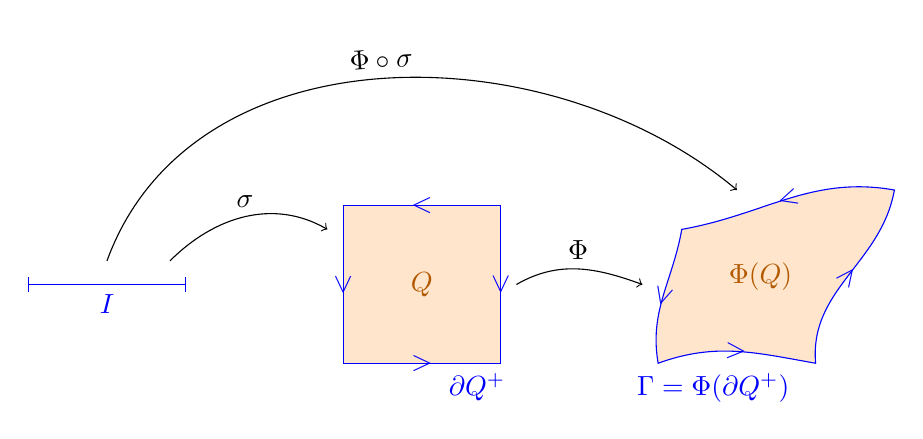
\begin{tikzpicture}
\draw[blue,|-|] (0,0) -- (2,0) node[midway,below] {$I$}; % Intervalo I

\draw[->] (1.8,0.3) to[out=45, in=150] node[midway,above] {$\sigma$} (3.8,0.7) ;

% % Primer cuadrado
\fill[orange!20!white,draw=none] (4,1) rectangle (6,-1);

\draw[blue] (4,-1) -- (4,1) node[midway,sloped] {\textless};
\draw[blue] (4,1) -- (6,1) node[midway,sloped] {\textless};
\draw[blue] (6,1) -- (6,-1) node[midway,sloped] {\textgreater};
\draw[blue] (6,-1) -- (4,-1) node[midway,sloped] {\textgreater};

\node[orange!70!black] at (5,0) {$Q$};
\node[blue,below] at (5.7,-1) {$\partial Q^+$}; 

\draw[blue, fill=orange!20!white] 
	(8,-1) to[out=100, in=260] node[midway,sloped] {\textless} 
	(8.3,0.7) to[out=10, in=170] node[midway,sloped] {\textless} 
	(11,1.2) to[out=260, in=95] node[midway,sloped] {\textgreater} 
	(10,-1) to[out=170, in=20] node[midway,sloped] {\textgreater}  (8,-1) -- cycle;

\draw[->] (6.2,0) to[out=30, in=160] node[midway,above] {$\Phi$} (7.8,0);	

\node[orange!70!black] at (9.3,0.1) {$\Phi(Q)$};
\node[blue,below] at (8.7,-1) {$\Gamma = \Phi(\partial Q^+)$};

\draw[->] (1,0.3) to[out=70, in=140] node[above,sloped] {$\Phi\circ\sigma$} (9,1.2);
\end{tikzpicture}
\caption{Esquema para la aplicación de Stokes en un cubo unidad}
\end{figure}

 Sea $\omega$ una k-forma en $\real^n$. Queremos calcular la integral de su diferencial en $Φ(Q)$.
 
\[
\int_{\Phi(Q)} \dif \omega = \int_Q \Phi^{\ast}\dif\omega = \int_Q \dif(\Phi^{\ast}\omega) = \int_{∂Q^{+}} \Phi^{\ast}\omega
\]

Donde $∂Q^{+}$ es la frontera del cubo $Q$ orientada debidamente. El último paso es aplicar el teorema anterior.

Sea $\appl{\sigma}{I}{∂Q}$. Entonces, $\appl{\Phi\circ\sigma}{I}{\Gamma}$, siendo $\Gamma$ la frontera de $\Phi(Q)$.

Aplicando esto a la integral que estamos calculando:

\[
\int_{\Phi(dQ^{+})} \omega \equiv \int{\Phi\circ\sigma(I)} = \int_I (\Phi\circ\sigma)^{\ast} \omega = \int_I \sigma^{\ast}\left(\Phi^{\ast}(\omega)\right) = \int_{\sigma(I)} \Phi^{\ast}\omega = \int_{∂Q}\Phi^{\ast}\omega
\]
Hemos llegado finalmente a que \[ \int_{∂Q^+} \Phi^{\ast} \omega = \int_{\Phi(∂Q^+)} \omega \]

Ahora querríamos dar el siguiente paso: 

\[\int_{\Phi(∂Q^+)} \omega = \int_{∂(\Phi^{\ast}(Q))} \omega \]

Es decir, que la imagen de la frontera sea la frontera de la imagen. Esto no es inmediato: en el cambio a coordenadas polares, por ejemplo, no se cumple a primera vista (ver figura \ref{imgCambioPolaresFrontera}). Cuando el ángulo (θ) se mantiene fijo y $r$ varía (segmentos azules), la imagen de esa parte de la frontera es un radio de la circunferencia, y cuando $r=0$ y variamos el ángulo (segmento verde) la imagen es un punto. 

\begin{figure}[hbtp]
\centering
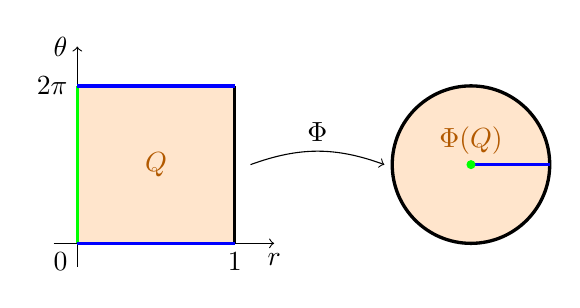
\begin{tikzpicture}
\fill[orange!20!white] (0,0) rectangle (2,2);

\draw[->] (0,-0.3) -- (0,2.5);
\node[left] at (0,2.5) {$\theta$};
\node[left] at (0,2) {$2\pi$};
\draw[->] (-0.3,0) -- (2.5,0);
\node[below] at (2.5,0) {$r$};
\node[below] at (2,0) {$1$};
\node[below left] at (0,0) {$0$};

\draw[very thick] (2,0) -- (2,2);
\draw[very thick,green] (0,0) -- (0,2);
\draw[very thick,blue] (0,2) -- (2,2);
\draw[very thick,blue] (0,0) -- (2,0);

\node[orange!70!black] at (1,1) {$Q$};

\draw[->] (2.2,1) to[out=20,in=160] node[midway,above,sloped] {$\Phi$} (3.9,1);

\draw[very thick,fill=orange!20!white] (5,1) circle (1);
\draw[very thick,blue] (5,1) -- (6,1);
\node[inner sep=1pt,circle,green,draw,fill=green] at (5,1) {};

\node[orange!70!black, above] at (5,1) {$\Phi(Q)$};

\end{tikzpicture}
\caption{La frontera no es la misma en el cambio a polares: las partes verde y azul forman parte de $∂Q$ pero no de $∂(Φ(Q))$.}
\label{imgCambioPolaresFrontera}
\end{figure}

Ahora bien, podemos dividir la región $Q$ en celdas disjuntas, como se puede ver en la figura \ref{imgPolaresDisjuntas}. De esta forma, las fronteras que sean comunes a varias celdas tendrán orientación incompatible y se anularán al integrar. Esto nos resuelve el problema y podemos enunciar el teorema de Stokes para celdas:


\begin{figure}[hbtp]
\centering
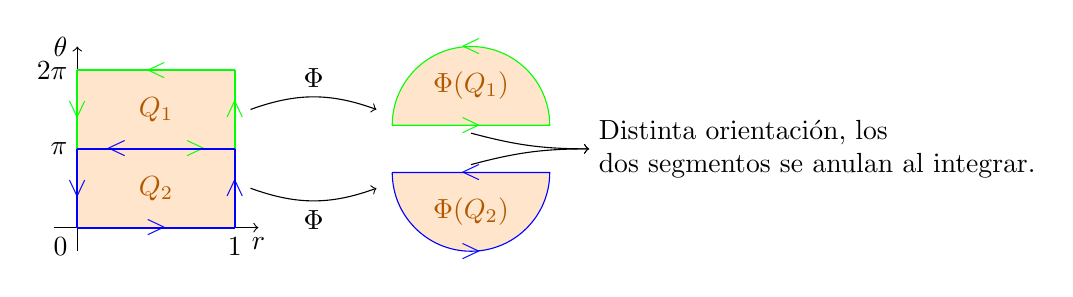
\begin{tikzpicture}
\fill[orange!20!white] (0,0) rectangle (2,2);

\draw[->] (0,-0.3) -- (0,2.3);
\node[left] at (0,2.3) {$\theta$};
\node[left] at (0,2) {$2\pi$};
\node[left] at (0,1) {$\pi$};
\draw[->] (-0.3,0) -- (2.3,0);
\node[below] at (2.3,0) {$r$};
\node[below] at (2,0) {$1$};
\node[below left] at (0,0) {$0$};

\draw[thick,green] (0,1) -- (0,2) node [midway,sloped] {\textless};
\draw[thick,green] (0,2) -- (2,2) node [midway,sloped] {\textless};
\draw[thick,green] (2,2) -- (2,1) node [midway,sloped] {\textless};
\draw[thick,green] (2,1) -- (0,1) node [near start,sloped] {\textgreater};

\draw[thick,blue] (0,0) -- (0,1) node [midway,sloped] {\textless};
\draw[thick,blue] (0,1) -- (2,1) node [near start,sloped] {\textless};
\draw[thick,blue] (2,1) -- (2,0) node [midway,sloped] {\textless};
\draw[thick,blue] (2,0) -- (0,0) node [midway,sloped] {\textgreater};

\node[orange!70!black] at (1,1.5) {$Q_1$};
\node[orange!70!black] at (1,0.5) {$Q_2$};

\draw[->] (2.2,1.5) to[out=20,in=160] node[midway,above,sloped] {$\Phi$} (3.8,1.5);
\draw[->] (2.2,0.5) to[out=-20,in=200] node[midway,below,sloped] {$\Phi$} (3.8,0.5);

\draw[green,fill=orange!20!white] (4,1.3) arc (180:0:1) -- (4,1.3) node[midway] {\textgreater};
\node[green] at (5,2.3) {\textless};
\node[orange!70!black] at (5,1.8) {$\Phi(Q_1)$};


\draw[blue,fill=orange!20!white] (4,0.7) arc (-180:0:1) -- (4,0.7) node[midway] {\textless};
\node[blue] at (5,-0.3) {\textgreater};
\node[orange!70!black] at (5,0.2) {$\Phi(Q_2)$};

\draw[->] (5,1.2) to[out=345, in=180] (6.5,1);
\draw[->] (5,0.8) to[out=15, in=180] (6.5,1);

\node[right,align=left] at (6.5,1) {Distinta orientaci\'{o}n, los\\ dos segmentos se anulan al integrar.};

\end{tikzpicture}
\caption{Podemos dividir $Q$ en dos celdas disjuntas}
\label{imgPolaresDisjuntas}
\end{figure}


\begin{theorem}[Teorema\IS de Stokes (para celdas)]\label{thmStokesCeldas}
\[ \int_M \dif \omega = \int_{\partial  M^+}\omega \]

, si la variedad $M$ se puede descomponer como unión de celdas con interior disjunto. 
\end{theorem} 

\paragraph{Frontera de una superficie}
Vamos a intentar definir en serio la frontera de objetos en $\real^3$, que es algo que necesitamos tener realmente muy claro.

\easyimg{imgs/StokesCeldasTipo.png}{ψ nos lleva $P$ a un punto que no está en la frontera de la imagen por ψ de su celda correspondiente (llamada de tipo I). En el caso de $Q$, ψ lo lleva a un punto en la frontera de la imagen de su celda por ψ (de tipo II), por lo tanto sí es un punto de la frontera.}{imgTiposCelda}

Hace un tiempo, cuando definíamos una subvariedad, demostramos la existencia de un difeomorfismo Ψ que "aplanaba un trozo" de subvariedad. La frontera de una superficie es el conjunto de los puntos (llamados en clase de Tipo 2) que al aplanar nos quedan en la frontera de un objeto de dimensión 2 (ver imagen \ref{imgTiposCelda}).
\index{Frontera}
Una vez aclarado el concepto de frontera, pasamos a demostrar el teorema de Stokes.


\begin{theorem}[Teorema\IS de Stokes]
Sea $M$ una subvariedad compacta, orientable, con frontera relativa $\partial  M$.

Entonces

\[\int_{\partial  M^+}\omega = \int_M \dif \omega \]

\end{theorem}

\begin{proof} La demostración ya está vista para celdas en la sección anterior, así que vamos a extender la idea.



\subparagraph{Paso 1: Compacidad}
Para todo punto $P\in M$ existe una celda $C_p$ tal que $P \in C_p$. Por lo tanto, está claro que $M\subset \bigcup_{p\in M} C_p$. Tomamos el interior de las celdas, para trabajar con conjuntos abiertos.

Hemos recubierto con infinitos abiertos la subvariedad, así que por compacidad (\ref{thmCerradoAcotado}) existe un subrecubrimiento \textbf{finito}.

Sin embargo, no podemos garantizar que las celdas son disjuntas. Si lo fueran, aplicaríamos el teorema a cada celda y listo. Hay que ver qué ocurre cuando las celdas no son disjuntas.

\subparagraph{Paso 2: Particiones de la unidad}

Vamos a intentar resolver el problema de los solapamientos. Buscamos una función que valga cero fuera de la celda que consideramos y sea mayor que cero dentro de ella, algo como pueda ser la figura \ref{imgStokesPhi}.

\begin{wrapfigure}{r}{0.6\textwidth}
  \begin{center}
    \includegraphics[width=0.58\textwidth]{imgs/TeoremaStokes-PartUnidad.png}
  \end{center}
  \caption{La función Φ que buscamos sería algo así.}
  \label{imgStokesPhi}
\end{wrapfigure}
Sea $\appl{\Phi}{\real^N}{\real}$. Además, 
\begin{itemize}
\item $\Phi>0$ en $\mathcal{Q}$
\item $\Phi = 0$ en $\partial  \mathcal{Q}$
\item $\Phi = 0$ en $\real^N-\mathcal{Q}$
\item $\Phi\in C^1$.
\end{itemize}
Consideramos $\Phi_i = \Phi\circ\Psi_{p_i}$, siendo $\Psi_{p_i}$ el difeomorfismo que cubre la celda $p_i$, con $i=1,...,k$ y la lleva al cubo unidad ($\mathcal{Q}$).

Además, nos gustaría que la suma de todas las aplicaciones $Φ_i$ sobre un punto sea 1:

\[ \sum_i \Phi_{i}(\gx) = 1\;\forall \gx \in M\]

Aunque parece una cosa imposible, vamos a ver que es algo perfectamente factible:

\[\tilde{\Phi}(\gx) = \frac{\Phi_i (\gx)}{\sum_{i=1}{k}\Phi_i(\gx)}\]

Estas $\tilde{\Phi}_i$ satisfacen todas las propiedades que nos interesan.

\subparagraph{Paso 3: Descomposición del problema}

Lo que nosotros queremos es calcular $\int_M d\omega$. Tal y como habíamos definido $\tilde{Φ}$ antes, es obvio que sobre la variedad $M$ 
\[ \omega=\sum_i^k\tilde{\Phi}_i(x)\omega \]

Entonces 

\[\dif \omega = \sum_{i=1}^k \dif (\tilde{\Phi}_i,\omega) = \sum_{i=1}^k \left( \dif \tilde{\Phi}_i\y \omega + \tilde{\Phi}_i \dif \omega \right) =  \dif\left(\sum_i \tilde{\Phi}_i\right) \y \omega + \sum \tilde{\Phi}_i \dif \omega\]

Dado que $\sum_i \tilde{Φ}_i = 1$, $\dif\left(\sum_i \tilde{\Phi}_i\right) = 0$ y por lo tanto

\[ \dif \omega = \sum \tilde{\Phi}_i \dif \omega \]

Aplicando esto descomponemos:
\[\int_M \dif \omega = \sum_{i=1}^k \int_M \tilde{\Phi}_i \dif\omega = \sum_{i=1}^k \int_{C_{p_i}} \tilde{\Phi}_i \dif\omega=\sum_{i=1}^k \int_{C_{p_i}} \dif(\tilde{\Phi}_i\omega)
\]

Hemos conseguido definir la integral como una suma finita de integrales sobre celdas en las que sí podemos aplicar el teorema de Stokes (\ref{thmStokesCeldas})

Entonces tenemos:

\[\int_M \dif \omega = \sum_{i=1}^k \int_{\partial  C_{P_i}^{+}} \tilde{\Phi}_i\omega\]

Por como hemos definido $\tilde{\Phi}_i$ tenemos que todas las celdas de tipo 1 valen 0. En cambio en las celdas de tipo 2 (ver \ref{imgTiposCelda} para los tipos de celda), tenemos una parte sobre la que $\tilde{\Phi}_i \neq 0$ (ver figura \ref{imgStokesCeldasIntegral}).

Esto nos deja: \[\int_M d\omega = \sum_{i=1}^k \int_{\partial  C{P_i}^{+}} \tilde{\Phi}_i\omega = \sum \int_{\partial M^+} \tilde{\Phi}_i \omega = \int_{\partial M^+} \omega\]

\end{proof}

\begin{figure}[hbtp]
  \begin{center}
    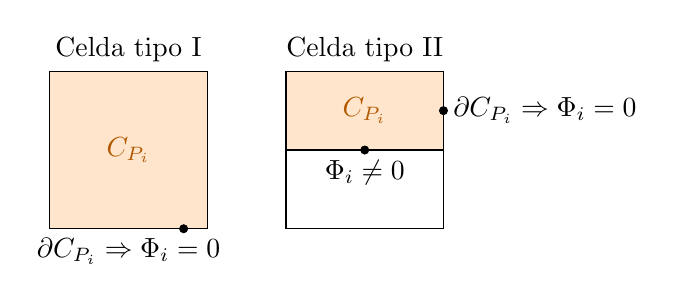
\begin{tikzpicture}
\draw[fill=orange!20!white] (0,0) rectangle (2,2);
\node[orange!70!black] at (1,1) {$C_{P_i}$};
\node[below] at (1,0) {$\partial C_{P_i} \Rightarrow \Phi_i = 0$};
\node[draw,circle,inner sep=1pt,black,fill=black] at (1.7,0) {};
\node[above] at (1,2) {Celda tipo I};

\draw[fill=white] (3,0) rectangle (5,2);
\draw[fill=orange!20!white] (3,1) rectangle (5,2);
\node[draw,circle,inner sep=1pt,black,fill=black] at (4,1) {};
\node[orange!70!black] at (4,1.5) {$C_{P_i}$};
\node[right] at (5,1.5) {$\partial C_{P_i} \Rightarrow \Phi_i = 0$};
\node[draw,circle,inner sep=1pt,black,fill=black] at (5,1.5) {};
\node[below] at (4,1) {$\Phi_i \neq 0$};
\node[above] at (4,2) {Celda tipo II};

\end{tikzpicture}
  \end{center}
  \caption{Sólo influyen a la integral los puntos de la frontera de la variedad, los que llevan a celdas de tipo II.}
  \label{imgStokesCeldasIntegral}
\end{figure}

\begin{example}
Sea $M$ una superficie en $\real^3$, un trozo de $x^2+y^2+z^2 = 1$ dentro de $x^2+y^2\leq y$, con $z\geq 0$. Ver figura \ref{imgEsferaCono}. Consideramos la orientación positiva como la de la normal hacia abajo.

\easyimg{imgs/EsferaCilindro.png}{Intersección de la esfera y el cilindro. La línea azul es la frontera de $M$, y las flechas naranjas indican su orientación positiva.}{imgs/EsferaCono}


Calcular las tres integrales

\[ \int_{\partial M} x \id y;\;\int_{\partial M} y \id z;\; \int_{\partial M} z \id x \]

\textbf{Previos} Nos damos cuenta de que $x^2+y^2\leq y$ es una circunferencia. Si completamos cuadrados tenemos la siguiente ecuación: \[x^2+\left(y-\frac{1}{2}\right)^2 = \frac{1}{4}\]

Es decir, una circunferencia de radio $\frac{1}{2}$ centrada en $(0,\frac{1}{2})$.

\paragraph{Resolución de $\int_{\partial M} x \dif y$}

\[
\int_{\partial M^{+}} x\dif y =\int_{\partial M^{+}} (0,x,0) \dif\sigma \stackrel{\mathrm{Stokes} }{=} \iint\limits_M \rot (0,x,0) \dif S = \iint\limits_M (0,0,1) \dif S
\]

Para calcular esta integral (que es calcular el flujo) aplicamos la fórmula de siempre. Para ello necesitamos parametrizar la superficie $M$:
\begin{equation}\label{eqEjStokes}
\Phi(x,y) = (x,y,\sqrt{1-x^2+y^2}), (x,y)\in D = \{x^2+y^2\leq y\} 
\end{equation}

Calculamos $T_x\x T_y =\displaystyle \left(\frac{x}{\sqrt{\cdot}},\frac{x}{\sqrt{\cdot}},1\right)$

\[
\int \int_M (0,0,1) dS = - \int \int_D \pesc{(0,0,1),(\ast,\ast,1)} \,dx\,dy = -\text{ Area } (D) = -\pi\frac{1}{4}
\]

\[ \int_{∂M^+}y\df{z} = \int_{∂M^+}(0,0,y)\df{σ} \stackrel{Stokes}{=} \int\int_{M^+} \rot (0,0,y)\df{S} \]

En \ref{eqEjStokes} teníamos la parametrización, así que la aplicamos. Teniendo en cuenta la orientación, tenemos que cambiar el signo y nos queda 

\[ 
- \iint_D \pesc{(1,0,0),\left(\frac{x}{\sqrt{\ast}}, \frac{y}{\sqrt{\ast}}, 1}\right) \df{x}\df{y} 
= -\iint_D\frac{x}{\sqrt{1-x^2-y^2}} \d{x,y} 
\]

Viendo que estamos integrando una función impar en una región simétrica, la integral vale 0.

\paragraph{Resolución de $\int_{\partial M} z \dif x$}

Pasamos ahora a calcular la integral de $z$. Tenemos lo mismo que antes:

\begin{gather*}
 \int_{∂M^+}z\df{x} = \int_{∂M^+}(z,0,0)\df{σ} \stackrel{Stokes}{=} \iint_{M^+} \rot (z,0,0)\df{S} = \iint_{M^+}(0,1,0)\id{S}= \\
 - \iint_D \pesc{(0,1,0),\left(\frac{x}{\sqrt{\ast}}, \frac{y}{\sqrt{\ast}}, 1\right)}\id{x,y} 
= -\iint_D\frac{y}{\sqrt{1-x^2-y^2}} \id{x,y}
\end{gather*}

Vemos que esta integral es muy complicada y nos va a ganar, así que pasamos a tratar de integrar como una curva. Deberemos parametrizar la curva, encontrar la orientación correcta y aplicar la fórmula.

Empezamos con la parametrización:

\[ ∂M = \left\{ \begin{matrix}
x^2+y^2+z^2 = 1 \implies y + z^2 = 1 \implies z = \sqrt{1-y} \\
x^2 + y^2 = y \implies x = \pm \sqrt{y-y^2}
\end{matrix}\right. \]

Por lo tanto, podemos parametrizar en dos trozos

\begin{align*}
Γ_1\equiv &(\sqrt{y-y^2}, y, \sqrt{1-y});\;y∈[0,1] \\
Γ_2\equiv &(-\sqrt{y-y^2}, y, \sqrt{1-y});\;y∈[0,1] \\
\end{align*}

\easyimgw{imgs/OrientacionesEsferaCilindro}{Orientaciones de $Γ_1$ y $Γ_2$}{imgs/OrientacionesEsferaCilindro}{0.7}

Tal y como vemos en la figura \ref{imgOrientacionesEsferaCilindro}, la orientación es negativa en $Γ_1$ y positiva en $Γ_2$. Entonces

\[ \int_{∂M^+}(z,0,0)\df{σ} = \int_{Γ_1^+}(z,0,0)\dif{σ_1} +  \int_{Γ_2^+}(z,0,0)\dif{σ_2} \]

Operando con la primera integral:

\[  \int_{Γ_1^+}(z,0,0)\dif{σ_1} = - \int_0^1\pesc{(\sqrt{1-y},0,0),\left(\frac{1-2y}{2\sqrt{y-y^2}},\ast,\ast\right)}\dif y = 
-\int_0^1\frac{1-2y}{2\sqrt{y}}\dif y = \]

Separamos en dos sumandos

\[ = \int_0^1\sqrt{y}\d y - \int_0^1 \frac{1}{2\sqrt y}\dif y = \dotsb \]

Podríamos tomar otra parametrización alternativa usando coordenadas esféricas. La esfera queda determinada por la parametrización

\[ \left\{\begin{matrix}
x &=& \cos θ \sin φ \\
y &=& \sin θ \sin φ \\ 
z &=& \cos φ
\end{matrix}\right. \]

Añadiendo la restricción de $x^2+y^2=y$, nos queda que $\sin φ = \sin θ$. Entonces podemos seguir parametrizando 

\[\left. \begin{matrix}
x = \cos θ \sin θ \\
y = \sin^2 θ \\
 z = \sqrt{1-\sin^2 θ} = \abs{\cos θ}
\end{matrix} \right\} θ∈[0,π]
\]

y tenemos que

\[ σ_1(θ) = (\cos θ \sin θ, \sin^2 θ, \cos θ) \]

Por otra parte, si pusiésemos los límites de integración en la región D pasaría algo.
\end{example}

\section{Campos conservativos}

\begin{defn}[Campo\IS conservativo] Consideramos $\vf$, un campo en $ℝ^N$. Se dice que $\vf$ es conservativo si y sólo si $∃\appl{V}{ℝ^N}{ℝ}$ tal que $F=\grad V$, donde $V$ es el \textbf{potencial}\index{Potencial} del campo $\vf$.
\end{defn}

\begin{theorem} Sea $\vf$ un campo $C^1$ en $ℝ^3$. Entonces $\vf $ es conservativo si y sólo si $\rot \vf = \vec{0}$.
\end{theorem} \label{consImpRot}

\begin{proof}
\paragraph{Implicación a la derecha} Como $F=\grad V$, y $F∈C^1$, entonces $V∈C^2$. Calculamos ahora el rotacional:

\[ \rot\vf = \left|\begin{matrix}
\vec{i} & \vec{j} & \vec{k} \\
\pd{}{x} & \pd{}{y} & \pd{}{z} \\
F_1 & F_2 & F_3
\end{matrix}\right| = \left(\dpa{F_3}{y}-\dpa{F_2}{z}, \dpa{F_1}{z}-\dpa{F_3}{x}, \dpa{F_2}{x}-\dpa{F_1}{y} \right) \]

Sustituyendo con $F=\grad V$ veríamos que sale todo cero.

\paragraph{Implicación hacia la izquierda}

Supongamos $Γ$ una curva cerrada, que sea la frontera de una superficie $M$. Entonces

\[ \int_{M^+}\vf  \stackrel{Stokes}{=} \iint_M\rot \vf\dif S = 0 \]

Es decir, que la integral de $F$ sobre cualquier curva cerrada va a dar 0. Buscamos ahora un $V$ tal que $\grad V = \vf$.

Supongamos un punto cualquiera $(x,y,z)$: A ese punto podemos llegar a través de varias rectas paralelas a los ejes. Con esas rectas podríamos construir un camino, y entonces tendríamos que 

\todo[inline]{Poner dibujito aquí}

\[ \int_{Γ_1}\vf = \int_{Γ_2} \vf = \int_{Γ_3}\vf \]

ya que cogiendo dos pares $Γ_i$ y cambiando la orientación de uno de ellos construimos una curva cerrada.

Parametrizamos $Γ_1$:

\[ Γ_1 \equiv \{ (t,0,0)\,t∈[0,x]\} 
	\cup \{ (x,s,0)\,s∈[0,y]\}
	\cup \{ (x,y,r)\,r∈[0,z]\} \]
	
Entonces

\begin{align*}
\int_{Γ_1}\vf&= \int_0^x\pesc{(F_1(t,0,0),F_2(t,0,0), F_3(t,0,0),(1,0,0)}\dif t \\
&+\int_0^y\pesc{(F_1(x,s,0),F_2(x,s,0), F_3(x,s,0),(0,1,0)}\dif s \\
&+\int_0^x\pesc{(F_1(x,y,r),F_2(x,y,r), F_3(x,y,r),(1,0,0)}\dif r \\
&=\int_0^x F_1(t,0,0)\dif t + \int_0^y F_2(x,s,0)\dif s+ \int_0^z F_3(x,y,r)\dif r 
\end{align*}

De la misma forma, tendríamos

\begin{gather*}
\int_{Γ_2}\vf = \int_0^y F_2(0,t,0)\dif t + \int_0^z F_3(0,y,s)\dif s+ \int_0^x F_1(x,y,r)\dif r \\ 
\int_{Γ_3}\vf = \int_0^x F_1(t,0,0)\dif t + \int_0^z F_3(x,0,s)\dif s+ \int_0^y F_1(x,r,z)\dif r \\
\end{gather*}

Las tres integrales son iguales, así que podemos derivar con respecto de la que nos venga mejor para construir la función $V$, que es la que buscábamos.

\end{proof}

La versión de este teorema vista en clase de prácticas (que es una versión más práctica)
\begin{theorem}[Campos conservativos]
$F$ es un campo vectorial $C^1$ en $\real^3$ excepto en un número finito de puntos entonces son equivalentes:
\begin{itemize}
\item Existe un potencial
\item La integral sobre una curva cerrada simple es 0
\item Las integrales por un camino o por otro para llegar a un punto son iguales
\item rot $\vf=0$.
\end{itemize}
\end{theorem}

Además, para calcular el potencial se puede utilizar cualquiera de estas 3 fórmulas:

\begin{gather*}
\int_{Γ_1}\vf=\int_0^x F_1(t,0,0)\dif t + \int_0^y F_2(x,s,0)\dif s+ \int_0^z F_3(x,y,r)\dif r \\
\int_{Γ_2}\vf = \int_0^y F_2(0,t,0)\dif t + \int_0^z F_3(0,y,s)\dif s+ \int_0^x F_1(x,y,r)\dif r \\ 
\int_{Γ_3}\vf = \int_0^x F_1(t,0,0)\dif t + \int_0^z F_3(x,0,s)\dif s+ \int_0^y F_1(x,r,z)\dif r \\
\end{gather*}

\subsection{Ejemplos}

\begin{example} Tenemos un cono de base $D$ y altura $h$, y buscamos integrar el campo $\vf(x,y,z)= (x,y,z)$. $Ω$ es el espacio del cono, y $∂Ω$, su superficie, se divide en la superficie lateral y la base.

\todo[inline]{Dibujito L1244}

Si escribimos el teorema de Gauss, tenemos que 

\[ \iiint_Ω \dv \vf \id{x,y,z} = \iint_{∂Ω^+} \vf \dif S \]

En este caso, tenemos la suerte de que $\dv \vf = 3$, y por lo tanto

\[ \iiint_Ω \dv \vf \id{x,y,z} = 3 \cdot \mathrm{Volumen}\,(Ω) \]

Por lo tanto, para hallar el volumen calculamos la integral sobre la superficie y dividimos entre tres.

La idea geométrica es que en la cara lateral, la componente normal de $\vf$ es 0. Lo vemos fácilmente sabiendo que la recta definida por el vector $(x,y,z)$ y que pasa por el origen (el vértice del cono), tiene exactamente la misma dirección de la generatriz. Entones,\textbf{ la integral sobre la cara lateral es 0} y por lo tanto podemos ignorarla. Nos centramos sólo en la integral de la base:

\[ \iint_{\mathrm{Base}}\vf \id S \]

Parametrizar $S$ es sencillo:

\[ S \equiv \{ (x,y,h)\tq (x,y)∈ D \} \]

Calculamos su vector normal:

\[ \left.\begin{matrix}
T_x = (1,0,0) \\
T_y = (0,1,0)
\end{matrix}\right\} T_x × T_y = (0,0,1) \]

y entonces

\[ \iint_{\mathrm{Base}}\vf \id S = \iint_D\pesc{(x,y,h),(0,0,1)} \id{x,y} = \iint_D h \id{x,y} = h \cdot \mathrm{Area}\,(D) \] 

Finalmente 

\[ \mathrm{Volumen}\,(Ω) = \frac{h \cdot \mathrm{Area}\,(D)}{3} \]
\end{example}

\begin{example}[Cálculo del campo eléctrico o gravitatorio]

La expresión del campo eléctrico es 

\[ \vf(\vx) = C \frac{\vx}{\norm{\vx}^3} \]

Calculando las derivadas parciales

\begin{align*}
\dpa{F_1}{x}&=\frac{y^2+z^2-2x^2}{(x^2+y^2+z^2)^{\frac{5}{2}}} \\
\dpa{F_2}{y}&=\frac{x^2+z^2-2y^2}{(x^2+y^2+z^2)^{\frac{5}{2}}} \\
\dpa{F_3}{z}&=\frac{x^2+y^2-2z^2}{(x^2+y^2+z^2)^{\frac{5}{2}}}
\end{align*}

nos queda que

\[ \dv\vf = 0 \]

Consideramos ahora una bola de radio $R$ centrada en el origen, es decir, $B_R(0,0,0)$. Integramos sobre su superficie:

\[ \iint\limits_{∂B_R^+} \vf \id{S} = 
\iint\limits_{x^2+y^2+z^2 = R^2} \left(\frac{x}{R^3},\frac{y}{R^3},\frac{z}{R^3} \right) \id S = \frac{1}{R^3} \iint\limits_{x^2+y^2+z^2 = R^2} (x,y,z)\id S = \]

Dado que integrar el vector es integrar su componente escalar, la integral nos queda

\[ = \frac{1}{R^3} \iint\limits_{x^2+y^2+z^2 = R^2} R\id{x,y} = \frac{1}{R^2}\cdot \mathrm{Area\; esfera} = 4π \]

Ahora bien, si no supiésemos ese argumento geométrico, empezaríamos parametrizando la esfera:

\[ Φ(θ,φ) =(R\cos θ \sin φ, R\sin θ\sin φ, R\cos φ);\, θ∈[0,2π], φ∈[0,π] \]

Calculamos los vectores tangentes y el normal:

\[ \left. \begin{matrix}
T_θ = (-R\sin θ \sin φ, R\cos θ \sin φ, 0) \\
T_φ = (R\cos θ\cos φ, R\sin θ \cos φ, -R\sin φ)
\end{matrix}\right\} T_θ×T_φ = -R\sin φ (R\cos θ, \]

La normal es interior, así que pagamos con un cambio de signo:

\begin{gather*} \iint\limits_{x^2+y^2+z^2 = R^2} \left(\frac{x}{R^3},\frac{y}{R^3},\frac{z}{R^3} \right) \id S = \\
- \int_0^{2π}\int_0^π\pesc{\left(\frac{R\cos θ \sin φ}{R^3},{R\sin θ \sin φ}{R^3},{R\cos φ}{R^3}\right), (,,)} = \dotsb \mathrm{Calculos\; aqui} \end{gather*}

y al final sale lo mismo que antes pero con cuentas mucho más desagrable.

¿Por qué el teorema de Gauss no funciona? La divergencia es 0 y la superficie es cerrada. Sin embargo, $\vf$ no es $C^1$ en el origen (no existe en ese punto) así que no podemos aplicarlo.

Pero, por otra parte, siempre hemos visto que la integral no se ve afectada por lo que ocurra en un punto. ¿Por qué no funciona el teorema de Gauss sólo por lo que pasa en el origen?

En realidad en el origen la divergencia vale $4π$ por un churrumillo muy raro (delta de algo) \todo{Dibujar el churrumillo}

Pero también podemos hacer un apaño. Consideramos un conjunto $Ω$, y una bola $B_ε(0,0,0)$. Entonces

\[ Ω_ε = Ω - B_ε \]

de tal forma que $\vf∈C^1$ en $Ω_ε$. Aplicando el teorema de Gauss:

\[ 0 = \iiint\limits_{Ω_ε}\dv \vf \id{x,y,z} = \iint\limits_{∂Ω_ε^+}\vf \id{S} \]

La frontera se divide en dos partes: $∂Ω_ε = ∂Ω + ∂B_ε^+$. Entonces

\[ 0 = \iint\limits_{∂Ω^+}\vf \id S - \iint\limits_{∂B_ε^+}\vf \id S \]

y por lo tanto, tenemos que 

\[ \iint\limits_{∂Ω^+}\vf \id{S} = 4π\; ∀Ω \tq 0 ∈ Ω \]

\end{example}


\begin{theorem}
Si $\vf \in C^1$

div$\vf = 0\dimplies \exists \vg\in C^2 \tlq \rot \vg = \vf$
\end{theorem}

\begin{proof}

Con el lenguaje de las formas diferenciales es muy facil esta demostración.

\todo[inline]{reescribir bien}
$vf$ es una 1-forma a la que aplicamos la diferencial exterior y obtenemos una 2-forma, que es su rotacional. Entonces, al volver a hacer la diferencial (para hallar la divergencia) es diferencial de diferencial =0.


Sin formas diferenciales tenemos:

\[G=(G_1,G_2,G_3)\]
\[\rot G = \left(\ast_1,\ast_2,\ast_3\right)\]

\[\div(\rot G) = \dpa{}{x}(\ast_1) + \dpa{}{y}(\ast_2) + \dpa{}{z}(\ast_3)\]
Por la igualdad de las derivadas cruzadas (toerema de Euler) al ser $G\in C^2$ se cancela todo.

$\implies$ Buscamos $\vg$ tal que $(F_1,F_2,F_3) = \rot \vg$.

Podemos definir el sistema:

\[\begin{array}{cc}
\dpa{G_3}{y} - \dpa{G_2}{z} &= F_1\\
\dpa{G_1}{z} - \dpa{G_3}{x} &= F_2\\
\dpa{G_2}{x} - \dpa{G_1}{y} &= F_3
\end{array}\]

Supongamos que $G_3\equiv 0$
\todo[inline]{Porque podemos suponer esto?}

\[\begin{array}{cc}
 - \dpa{G_2}{z} &= F_1\\
\dpa{G_1}{z} - &= F_2\\
\dpa{G_2}{x} - \dpa{G_1}{y} &= F_3
\end{array} \begin{array}{cc}
\longrightarrow & G_2 = -\int_0^z F_1(x,y,t)dt+A(x,y)\\
\longrightarrow & G_1 = \int_0^2 F_2(x,y,t)dt + B(x,y)\\
\longrightarrow & F_3 = \dpa{}{x} \left\{-\int_0^z F_1(x,y,t)dt + A(x,y)\right\}
- \dpa{}{y}\left\{\int_0^2 F_2(x,y,t)dt + B(x,y) \right\}
\end{array}
\]

Vamos a ver que ocurre con  $F_3$

\[-\dpa{}{x}\left(\int_0^z F_1(x,y,t)dt\right) + \dpa{A}{x} - \dpa{}{y}\int_0^z F_2(x,y,t)dt - \dpa{B}{y}\]

Por la regularidad de $F_1$ podemos meter dentro la derivada (el argumento que está detrás de esto se ve en teoría de la medida, asíque de momento nos fiamos)

\[-\left(\int_0^z \dpa{}{x}F_1(x,y,t)dt\right) + \dpa{A}{x} - \int_0^z \dpa{}{y}F_2(x,y,t)dt - \dpa{B}{y}\]
\[-\int_0^z \left(\dpa{F_1}{x} + \dpa{F_2}{y}\right)(x,y,t)dt + \dpa{A}{x} - \dpa{B}{y} \]

Utilizamos que la $\dv = 0$ que nos dice:

\[\dpa{F_1}{x} + \dpa{F_2}{y} + \dpa{F_3}{z} = 0\]

\[ = \int_0^z \dpa{F_3}{z} (x,y,t)dt + \dpa{A}{x} - \dpa{B}{y} = F_3(x,y,z) - F(x,y,z) + \dpa{A}{x} - \dpa{B}{y}\]

Hemos llegado a \[F_3(x,y,z) =  F_3(x,y,z) - F(x,y,z) + \dpa{A}{x} - \dpa{B}{y}\]
Quedando entonces definidas $A$ y $B$ así:

\[\dpa{A}{x} - \dpa{B}{y} = F_3(x,y,0)\]
Y aquí nuevamente tenemos muchas opciones. Elegimos/suponemos/tomamos $B=0$ 
\todo[inline]{porque?}

\[A(x,y) = \int_0^x F_3(s,y,0)ds + C(y)\]
\end{proof}

\subsubsection{Anexo interesante}
Vamos a ver ahora un ejemplo de cuándo se pueden meter las derivadas dentro de una integral.

\begin{example}
Tenemos un sólido a una cierta temperatura, rodeado de un amniente a otra temperatura distitnta de tal manera que el sólido va perdiendo temperatura. Queremos saber a qué temperatura estará el sólido pasa un tiempo $T$.

Partimos de la interpretación de que la temperatura mide la \emph{cantidad de calor}. 

\textbf{Concepto previo} Una olla de 100 Litros y un vasito de chupito, ambos con agua a 100 grados, ¿qué recipiente tiene más energía? Respuesta: la olla porque es más grande.

\todo{creo que es así}
Podemos calcular el calor integrando la temperatura con el volumen


Siendo $\Omega$ el sólido, y $u(x,t)$ es la temperatura en $x$ en el instante $t$. Entonces:

\[\iiint u(x,t) dx \equiv \text{ Cantidad de calor en }\Omega\text{ en }t\]

Vamos a tomar una $B_{\epsilon}(x_0)$, vamos a estudiar:
\[\dpa{}{t} \iiint_{B_{\epsilon}(x_0)} u(x,t)dx\]
 Es la variación de temperatura a lo largo del tiempo. La temperatura varía porque el calor se transmite. ¿De qué manera se transmite? Sale fuera a través de la frontera. Se habrá ganado el calor que haya entrado y se habrá perdido el calor que haya salido. ¡Es un flujo!
 (de un campo $\vec{J}$)
  
 \[\dpa{}{t} \iiint_{B_{\epsilon}(x_0)} u(x,t)dx = -\iint_{\partial B_{\epsilon}(x_0)} \vec{J}dS\]
 (El menos aparece porque queremos que la derivada sea negativa, porque el calor sale.)
 
 
 Siguiendo la idea de Leibniz de que estamos en el mejor mundo posible ,porque el calor se transmite de las zonas calientes a las zonas frías de la manera óptima, es decir, en la dirección del $-\grad$.
 
 \todo[inline]{Revisar que pasa con $\dpa{}{t}$}
 
 \[\dpa{}{t} \iiint_{B_{\epsilon}(x_0)} u(x,t)dx = -\iint_{\partial B_{\epsilon}(x_0)} \vec{J}dS = \iint_{\partial B_{\epsilon}(x_0)}\]
 \[ = -\grad_x u dS \stackrel{Gauss}{=} \iiint_{B_{\epsilon}(x_0)} \dv(\grad_x u) = \iiint_{B_{\epsilon}(x_0)}  \]

\[ = \iiint_{B_{\epsilon}(x_0)} \dpa{u}{t}-Au\,dx=0,\forall \epsilon\]

Como lo que integramos es continua (lo llamamos $f$)

Tenemos:
\[m_{\epsilon} \leq \frac{1}{Vol(B_{\epsilon})} \iiint f \leq M_{\epsilon}\] 

Si $\epsilon \to 0$ entonces $\displaystyle\iiint_{B_{\epsilon}(x_0)} f = f(x_0)$

Entonces tenemos que \[\dpa{u}{t}(x_0,t) - Au(x_0,t) = 0\]

Y de aquí deducimos las 3 ecuaciones de transmisión de calor, que son: 
\todo[inline]{no se cuales son}
 \end{example}

Para este ejemplo ha sido fundamental el meter dentro una derivada ($\dpa{}{t}$) dentro de la integral.

Ahora vamos a ver otro ejemplo en el que esto no se puede aplicar:

\begin{example}
\todo{Dibujo}
\[\int_0^1 f_n(x)dx = \frac{1}{2}\]
\[\lim_{n\to\infty}\int_0^1 f_n(x)dx = \frac{1}{2}\]
\[\int_0^1 \lim_{n\to\infty} f_n(x) = \int_0^1 0dx = 0\]

Estamos cometiendo un error... que no vamos a contar cuál es, que se verá en teoría de la medida.
\end{example}

Nos podemos plantear en qué condiciones es cierto (en el ejemplo anterior es falso):

\[\lim_{n\to\infty} \int_{\Omega}\frac{u(x,t+1/u)-u(x,t)}{1/u} \,dx = \int_{\Omega}\lim_{n\to\infty}\frac{u(x,t+1/u)-u(x,t)}{1/u} \,dx
\]

Lo primero que tenemos que definir es la \textbf{convergencia de una sucesión a una función.} Vamos a ver un plan de interpretaciones.

\subparagraph{\textit{Convergencia puntual}}

$\forall x\in\Omega$, dado un $\epsilon>0\\ \exists n_0 \tlq n>n_0 \implies \abs{f_n(x)-f(x)}<\epsilon$

\begin{example}
1) \[f(x) = \left\{\begin{array}{cc}
1 & x\in[0,1]\cap \rac\\
0 & x\in[0,1]\cap\{\real-\rac\}
\end{array}\right.\]
Este es el ejemplo de función no integrable por Riemman (las sumas superriores valen 1 y las sumas inferiores valen 0, debido a la numerabilidad de los Racionales)

2)
Nosotros podemos definir una función de la siguiente manera: 

\[f_n(x) = \left\{\begin{array}{cc}
1 & x=r_1,...,r_n\\
0 & x\in\real-\{r_1,...,r_n\}
\end{array}\right\}\]
Siendo $r_i\in\rac$. Como es un conjunto numerable podemos definir un orden.

Continua excepto en un nº finito de puntos $\implies$ integrable de Riemman.

3) $f_n(x)\to f(x) \forall x\in[0,1]$


\textbf{Conclusión} En este caso tenemos que la convergencia puntual podemos no tener integral. 
\end{example}

Para solucionar este problema podemos definir otra noción de límite que nos evite este problema u otra noción de integral.

\subparagraph{\textit{Convergencia uniforme}}

Dado $\epsilon>0\,\exists\,n_0=n_0(\epsilon) \tlq n_0>n_0 \implies \abs{f_n(x) - f(x)} < \epsilon\, \forall x\in\Omega$.

Es decir, ${sup}{x\in\Omega} \abs{f_n(x)-f(x)} = \md{f_n-f}_{\infty} <\epsilon$.

La misma idea que con continuidad uniforme, para todos los $x$ del intervalo nos vale el mismo $n_0$.

Utilizando esta definición en el ejemplo de los triángulos, no podemos definir la sucesión que sea convergente uniformemente.

\begin{theorem}[Convergencia uniforme]
Sea $\Omega$ un dominio acotado en $\real^N$. 

Si $f_n \to f$ converge uniformemente en $\Omega$

\textbf{entonces}
\[\lim_{n\to\infty} \int_{\Omega} f_n(x)\,dx = \int_{\Omega} \lim_{n\to\infty} f_n(x)\,dx = \int_{\Omega} f(x)\,dx\]

Es decir, el límite y la integral son intercambiables.
\end{theorem}

\begin{proof}
\[0\leq\abs{\int_{\Omega}f_n(x) - f(x) \, dx} \leq <\int_{\Omega} \epsilon \,dx =\epsilon\abs{\Omega} \to 0\]
\end{proof}

\begin{theorem}
\[\left.\begin{array}{cc}
\{f_n\} \text{ continua }\\
f_n \to f \text{ uniforme en } \Omega \end{array}
\right\} \implies f \text{ continua}\]
\end{theorem}
\obs Si tenemos convergencia unifirme, tenemos una función continua. Parace una cosa tan tan buena que incluso se pasa de buena, porque no podemos trabajar con discontinuidades

\obs Adelantamos un teorema de teoría de la medida que dice \textit{ Casi todas las funciones son casi continuas en casi todos los puntos}


\begin{proof}
\[\abs{f(x) - f(y)} = \abs{f(x) \pm f_n(x) \pm f_n(y) - f(y)}\]

Elegimos un subíndice $n$ para el que se cumpla $\abs{f_n(t) - f(t)} < \frac{\epsilon}{3}$

Además, como $f_n$ son continuas, tenemos que haciendo tender $x\to y \implies f(x) - f(y) \leq \epsilon \implies$ continuidad
\end{proof}


\paragraph{Aplicación}

Sea $f_n(x) = \frac{u(x,t+1/u) - u(x,t_0)}{1/u}$

$f(x) = \dpa{u}{u}(x,t_0)$

Vamos a comprobar la convergencia uniforme:

\[0\leq \abs{f_n(x) - f(x)} \leq \abs{\frac{u(x,t+1/u) - u(x,t_0)}{1/u} - \dpa{u}{u}(x,t_0)} \stackrel{TVM}{=} \abs{\dpa{u}{t}(x,s) - \dpa{u}{t}(x,t_0)} < \epsilon \forall x\]
Donde $s\in [t_0,t_0+\frac{1}{n}]$

En el último paso utilizamos la continudad de la derivada y la compacidad (que nos da continuidad uniforme)


\subparagraph{Integral de Lebesgue}
La otra opción para poder intercambiar límites con integrales podíamos ser más estrictos con la convergencia, o mejorar la integral (aparte de todo un mundo de posibilidades intermedias del \textit{Análisis funcional}) 

Algo de esto ya vimos al hablar de integrales: (\ref{IntLebesgue})

Esto nos genera el problema de la medida de un intervalo. 
Es razonable pedir:
\begin{itemize}
\item $\abs{(a,b)} = \abs{b-a}$
\item La medida del intervalo tiene que ser invariante si le aplicamos traslaciones
\item $A\cap B = Ø $

$\abs{A \cup B} = \abs{A} + \abs{B}$
\item $A_i \cap A_j = Ø, i\neq j$

$\abs{\bigcup_{i=1}^{\infty} A_i} = \sum_{i=1}^{\infty} \abs{A_i}$.


\end{itemize}
El último requisito es un verdadero dolor de cabeza, trabajar con sumas infinitas y con uniones infinitas. Sería fácil (con la medida exterior) para conseguir un $\leq$ que no es suficiente.

Para solucionar todo estos problemas hay que definir una nueva teoría con la que casi todo es medible (salvo unos cuantos monstruos, que para encontrarlos hay que hablar del Axioma de elección)

Toda esta teoría de la integral de Lebesgue nos da resultados mucho más generales para poder intercambiar el límite con la integral, con la convergencia monótona y la convergencia domiante.

\newpage

\appendix
\chapter{Resumen}
% Autor: Pedro Valero
%
% Este documento no es más que un resumen que he decidido hacer por mi cuenta
% y riesgo.
%
% No sustituye los apuntes de curso y en un principio no voy a subirlo a dropbox, es un resumen
% hecho por mi para mi, sin preocuparme de que vaya siendo claro para todos.
%
% Lo tengo en esta carpeta porque es la forma más cómoda de tenerlo a mano y guardado en git.

\documentclass{apuntes}

\title{Resumen de Lógica Matemática}
\author{Pedro Valero}
\date{15/15 C1}
% Paquetes adicionales
\usepackage{tikztools}
\usepackage{fastbuild}
\usepackage{tikz-3dplot}
\usepackage{fancysprefs}

\bibliographystyle{plainnat}

\usetikzlibrary{arrows}
% --------------------

\precompileTikz

\begin{document}
\pagestyle{plain}
\maketitle

\tableofcontents

\chapter{Lógica proposicional}

\section{Repaso de conceptos básicos de EDyL}
Siempre que que trabajemos con predicados de lógica proposicional empezaremos definiendo un lenguaje, que estará compuesto por un alfabeto y un conjunto de símbolos (conectores).

\[L \equiv A\cup\{\neg,\implies, \wedge, \vee, \iff, \perp, \top, ), ( \}\]

\begin{defn}[Proposición o fórmula bien formada]
	Palabra (concatenación de símbolos) que pertenece a la clase más pequeña cerrada bajo las siguientes propiedades:
	\begin{itemize}
		\item Los elementos de $A$, $\perp$ y $\top$ son fórmulas atómicas (no se pueden dividir).
		\item Si $F_1$ y $F_2$ son fórmulas, también lo son
		\begin{itemize}
			\item $(\neg F_1)$
			\item $(F_1\implies F_2)$
			\item $(F_1\iff F_2)$
			\item $(F_1\wedge F_2)$
			\item $(F_1\vee F_2)$
		\end{itemize}
	\end{itemize}
\end{defn}

Las fórmulas bien formadas pueden definirse de manera inductiva:
\begin{equation*}
\begin{array}{l l l}
	\textbf{FBF}_\textbf{0} &=& A\cup\{\top, \perp \}\\
	\textbf{FBF}_\textbf{n+1} &=& FBF_n \cup \{(\neg F_1), (F_1\implies F_2),(F_1\iff F_2),(F_1\wedge F_2),(F_1\vee F_2)\}\\ &&\text{con } F_1,F_2\in \textbf{FBF}_\textbf{n}.
\end{array}
\end{equation*}

\begin{lemma}[Legibilidad única]
Las fórmulas nunca son ambiguas, sólo pueden leerse o construirse de una forma, cualidad que conseguimos mediante el empleo de paréntesis.
\end{lemma}

Existe una serie de \concept{axiomas proposicionales}. Estos axiomas son FBF que son ciertas para cualquier interpretación de los elementos que las constituyen. Una \concept{Interpretación} es una función que dada una FBF nos devuelve un valor de verdad (Verdadero o Falso). De forma más fórmal, una interpretación es una valoración booleana
\[\appl{\sigma}{FBF(L)}{(\mathbb{Z}_2, +, \cdot)} \text{ que satisface } \]

\begin{itemize}
	\item $\sigma(\top) = 1$, $\sigma(\perp) = 0$
	\item $\sigma(\neg p) = 1+\sigma(p)$,  siendo $p$ una FBF.
	\item $\sigma (p\vee q) = \sigma(p) \vee \sigma (q) = \max\left\{\sigma(p), \sigma(q)\right\}$
	\item $\sigma (p\wedge q) = \sigma(p) \wedge \sigma (q) = \min\left\{\sigma(p), \sigma(q)\right\}$
\end{itemize}

Estos axiomas son empleados junto con la regla \textbf{modus ponens} para lograr demostrar la verdacidad de otras FBFs

\begin{mdframed}
\textbf{Notación}
\begin{itemize}
	\vspace{-3mm}
	\item Escribimos $\vdash p$ para denotar que existe una demostración de $p$.
	\item Escribimos $\vDash p$ para denotar que $p$ es verdad.
\end{itemize}
\end{mdframed}

Todo conjunto de FBFs se considera una \concept{Teoría}, independientemente de que sea una tautología o no.

\begin{defn}[Demostración o prueba (II)]
	Una demostración a partir de los axiomas y una teoría $T$ es una sucesión finita $p_1, \hdots, p_n$, donde cada $p_i$ es o un axioma, o $p_i\in T$ o se obtiene de dos $p_j,p_k$ anteriores mediante modus ponens.

	$T \vdash p$ indica que existe una demostración o prueba de $p$ a partir de $T$
\end{defn}

\begin{theorem}
	Sea $\appl{\sigma}{A}{\{0, 1\}}$ una función arbitraria. Entonces $\sigma$ se extiende, de modo único, a una valoración booleana $$\hat{\sigma}:FBF(L) \to \mathbb{Z}_2$$
\end{theorem}

\begin{defn}[Sistema completo]
Un sistema de conectivas es completo si a partir de ellas pueden deducirse las demás
\end{defn}

\begin{defn}[Modelo]
Una interpretación σ es un modelo de una teoria $T$ si y sólo si
\[\forall p \in T \ \ \ σ(p)=\top=1\]
\end{defn}

\begin{defn}[Consecuencia tautológica]
	Decimos que $p$ es una consecuencia tautológica de $T$, y escribimos $T\vDash p$, si para todo modelo $\sigma$ de $T$, $\sigma(p) = 1$. En este contexto, decimos que $p$ es una \textbf{tautología} y escribimos  $\vDash p$.
\end{defn}

\begin{defn}[Teoría consistente]
Decimos que una teoría $T$ es consistente si $T\nvdash \perp$. La consistencia o coherencia puede caracterizarse de forma sencilla:
 $$T\nvdash\perp \iff \exists p\in FBF(L) \tq  T\nvdash p$$
 Equivalentemente, una teoría $T$ es inconsistente si $T\vdash \perp$.
 $$T\vdash\perp \iff T\vdash p\ \forall p\in FBF(L)$$
\end{defn}

\begin{theorem}[Teorema de la deducción]
	Si $T\cup\{p\}\vdash q$, entonces $$T\vdash p\implies q$$
\end{theorem}

\section{Problemas TAUT y SAT}
\begin{defn}[Problema de las tautologías]
El \textbf{problema de la tautología} consiste en determinar si una FBF es una tautología, para lo que basta con calcular la tabla de verdad, labor que toma un tiempo exponencial en el tamaño del lenguaje empleado.
\end{defn}

\paragraph{Clases de complejidad}
\begin{itemize}
	\item \textbf{P:} clase de problemas para los que existe un algoritmo que los resuelve en tiempo polinómico en función del número de datos de entrada, es decir, $\exists K\ge 0$ (dependiendo el problema pero no del número de datos $n$) tal que si tenemos $n$ datos de entrada, el algoritmo requiere menos de $O(n^K)$ operaciones.
	\item \textbf{NP:} tiempo polinómico no determinista. Si tenemos una solución, podemos comprobar si es correcta (o no) en tiempo polinómico, pero no podemos generar la solución. Obviamente P$\subset$NP.
	\item La clase de problemas \textbf{NP-difícil} se define como aquella que contiene a los problemas que son como mínimo tan difíciles como un problema de NP. Alternativamente, se define como la clase de problemas H tal que todo problema en NP puede ser transformado polinomialmente en H.
	\item La clase de problemas \textbf{NP-completo} se define como la intersección entre la clase de problemas NP y la clase de problemas NP-difícil.
\end{itemize}
Se sabe que \textbf{TAUT} es NP-difícil, pero no se sabe si P$=$NP.

\begin{defn}[Problema de la satisfacción]
Este problema consiste en determinar si existe una interpretación que satisfaga una FBF dada. Se trata de un problema \textbf{NP-completo}
\end{defn}

\section{Completitud}
\begin{theorem}[Teorema de completitud]
Sea una teoría no vacía se tiene que:
\[T \vdash p \iff T \vDash p\]
\end{theorem}

Una teoría es \concept{consistente} si nunca prueba $p$ y $\neg p$ simultáneamente. En general, una teoría $T$ será \textbf{consistente} si existe alguna $p$ tal que $T \nvdash p$.

\begin{defn}[Teorería completa]
Una teoría es completa si es consistente y para toda FBF $p$, se cumple que $T \vdash p$ o $T \nvdash p$
\end{defn}

\begin{theorem}
	Si $T \nvdash p$, entonces $T\cup \{\neg p\}$ es consistente.
	\label{thm:pconsnegp}
\end{theorem}
\begin{proof}

	Vamos a reescribir lo que queremos probar como:
	\begin{center}``Si $T\cup \{\neg p\}$ es inconsistente, entonces $T\vdash p$''.\end{center}

	Si $T\cup \{\neg p\}$ es inconsistente podemos escribir
	\[T\cup \{\neg p\}\vdash \perp\]
	Por el teorema de la deducción
	\[T\vdash \neg p\implies \perp\]
	Por el axioma 8, que dice:
	\[(\neg p\implies \perp)\implies p\]
	tomando $(\neg p \implies \perp)\implies p$ y aplicando modus ponens, obtenemos $T\vdash p$.
\end{proof}

\begin{theorem}[Teorema de Lindenbaum]
	Toda teoría consistente puede extenderse a una teoría completa.
	\label{thm:lindenbaum}
\end{theorem}
\begin{proof}
	En esta demostración nos apoyaremos en el Lemma de Zorn.

	Sea $T$ una teoría consistente y sea $P$ el conjunto de todas las teorías consistentes que extienden a $T$, definimos un orden parcial en $P$ mediante inclusión:
	\[T_1\le T_2 \iff T_1\subset T_2\]

	Sea $\{T_\alpha\}_{\alpha\in\Lambda}$ una cadena en $P$.

	Si $\cup_{\alpha\in\Lambda} T_\alpha$ es consistente, entonces es una cota superior de la cadena.

	Puesto que todas las $T_\alpha$ son consistentes, la unión será consistente.
	\begin{proof}
	Queremos probar que:
	\[\bigcup_α T_α \vdash \perp \implies \exists α \ T_α \vdash \perp \equiv \forall α \ T_α \nvdash \perp \implies \bigcup_αT_α \nvdash \perp\]

	Realizaremos la prueba por reducción al absurdo.

	Sea $p_1,\hdots,p_n = \perp$ una prueba formal de $\perp$. Entonces, $\exists T_{\alpha_1}\vdash p_1$, $\exists T_{\alpha_2} \supset T_{\alpha_1}$ tal que $T_{\alpha_2}\vdash p_2, \hdots, T_{\alpha_n}\supset \exists T_{\alpha_{n-1}}$ tal que $T_{\alpha_n}\vdash p_n$.

	\obs Al final del ``procedimiento'' que acabamos de definir llegamos a una teoría $T_n$ que contiene a todos los $p_i$ y que, por tanto $T_n \vdash \perp$. Pero estábamos considerando que todas las $T_i$ eran consistentes, por lo que acabamos de llegar a una contradicción.

	Queda claro pues que la unión de teorías consistentes es consistente.
	\end{proof}

	Por el lema de Zorn sabemos que $P=\bigcup_αT_α$ tiene un elemento maximal $M$, que contiene a $T$. Por tanto $M\in P$, lo que implica que $M$ es consistente.

	Además, por ser $M$ maximal tenemos que $\forall p \ M \vdash p \Or M \vdash \neg p$ puesto que de no ser así, tanto $M\cup\{p\}$ como $M\cup\{\neg p\}$ serían consistentes y extenderían $T$ por lo que pertencerían a $P$. Puesto que $M$ es el elemento maximal de $P$ tenemos que $M\cup\{p\} \subset M \implies p \in M$ y $M\cup\{\neg p\}\subset M \implies \neg p \in M$ con lo que $M$ no sería consistente.

	Queda claro pues que $M$ es la extensión completa de la teoría que estábamos buscando.
\end{proof}


\begin{theorem}[Teorema de completitud II]
	$T$ es consistente $\iff$ $T$ tiene un modelo.
	\label{thm:comp2}
\end{theorem}

\begin{theorem}[Teorema de compacidad]
	Si todo subconjunto finito de una teoría $T$ tiene un modelo, entonces $T$ tiene un modelo.
\end{theorem}
\begin{proof}
	Como todo subconjunto finito de $T$ tiene un modelo, todo subconjunto finito es consistente, luego $T$ es consistente y por \ref{thm:comp2}, $T$ tiene un modelo.

	Para ver que $T$ es consistente sabiendo que todo subconjunto finito es consistente nos basta con ver que si $T\vdash \perp$, existe una demostración $p_1, \hdots, p_n = \perp$ usando las premisas en $T$. Pero $T\cap\{p_1,\hdots,p_{n-1}\}\vdash \perp$, por lo que no es consistente, y es finito, por lo que llegamos a una contradicción.
\end{proof}

\chapter{Lógica de órdenes superiores}
\section{Lógica de primer orden}
Asumimos que todos los conjuntos usados para definir el lenguaje son disjuntos. Usaremos:
\begin{itemize}
	\item \textbf{Símbolos} lógicos y de puntuación:
	$$\{\neg, \vee, ),(, ``," \}$$
	También usaremos los demás símbolos lógicos como abreviaciones.
	\item Tendremos un conjunto infinito numerable de \textbf{variables}:
	$$Var = \{v_1, v_2, \hdots\}$$
	Aunque en la práctica usaremos $x,y,z$.
	\item Un conjunto de constantes, que podría ser vacío:
	$$Con = \{C_0, C_1, \hdots\}$$
	\item Funciones:
	$$Fun = \{f_0, f_1, \hdots\}$$
	\item Relaciones o predicados:
	$$Rel = \{R_1, R_2, \hdots\}$$
	\item Cuantificadores:
	$$\{\forall, \exists\}$$
	Podemos considerar $\exists x(P(x))$ como abreviación de $\neg (\forall x(\neg P(x)))$.
\end{itemize}

\subsection{Los números naturales}
\begin{defn}[Los naturales]
	\begin{itemize}
		\item $0:=\emptyset$
		\item $1:=\{\emptyset\}$ (por emparejamiento o partes cuando lo veamos).
		\item $2:=\{\emptyset, \{\emptyset\}\} = \{0,1\}$ (por emparejamiento).
		\item $3:=\{1,2,3\} = \{\emptyset,\{\emptyset\},\{\emptyset, \{\emptyset\}\}\}$ (Por el axioma 4).
	\end{itemize}
	\end{defn}

	\begin{defn}[Sucesor]
		El sucesor de $n$, $S(n)$ es $$S(n) = \{0,1,2,\hdots, n\}$$
	\end{defn}

	\begin{defn}[Suma en los naturales]
		$n+1 := S(n)$. Si hemos definido $n+m$, entonces
		$n+m+1 := S(n+m)$.
	\end{defn}

	\obs A partir de aquí podemos definir todo $n\in \nat$ como un conjunto, pues $n=S(n-1)=\{0,1,...,n-1\}$

	\begin{defn}[Producto de los naturales]
		En cuanto al producto:
		\begin{itemize}
			\item $n\cdot0 = 0$
			\item $n\cdot1=n$
			\item Si $n\cdot m$ está definido, entonces $n(m+1) = n\cdot (m+1) = n\cdot m + n$.
		\end{itemize}
	\end{defn}

	\begin{defn}[Menor]
		$$n<m\iff n\in m$$
	\end{defn}

\subsection{Axiomas de Peano}
	Los 5 Axiomas de Peano son:
	\begin{enumerate}
		\item Existe un número natural 1. En otros términos, 1 está en N, el conjunto de los números naturales.
		\item Todo número natural n tiene un sucesor n* (este axioma es usado para definir posteriormente la suma).
		\item 1 no es el sucesor de algún número natural.
		\item Si hay dos números naturales n y m con el mismo sucesor, entonces n y m son el mismo número natural.
		\item Si 1 pertenece a un conjunto K de números naturales, y dado un elemento cualquiera n, el sucesor n* también pertenece al conjunto K, entonces el conjunto K debe ser el conjunto de todos los números naturales. Este axioma es el principio de inducción matemática.
	\end{enumerate}

\section{Lógica de segundo orden}
\begin{theorem}\label{theorem:todo_sub_finito_modelo}
Existe una teoría T en un lenguaje de 2º orden, tal que, todo subconjunto finito de T tiene un modelo, pero T no tiene ningún modelo.
\end{theorem}
\begin{proof}
Si consideramos la teoría $\Psi_{\infty}$, donde $\Psi_{\infty}$ nos dice que existe una función inyectiva que no es sobreyectiva, vemos que todos sus modelos son infinitos (todas las funciones que satisfacen la teoría deben moverse entre conjuntos infinitos.)
$$ \Psi_{\infty}: \exists f \left(\forall x \textbf{ } \forall y \left( \left( f(x)=f(y)\right) \Rightarrow x=y \right) \y \left( \exists z \forall x \left( z \neq f(x) \right) \right) \right) $$


Por otro lado, es claro que todo modelo de $\neg \Psi_{\infty}$ es finito.

Vamos a considerar el conjunto de teorías $\Psi_n$, cada una de las cuales nos dice que por lo menos hay n objetos distintos:
$$ \Psi_2: \exists v_1 \exists v_2 \left(v_1 \neq v_2 \right) $$
$$ \Psi_3: \exists v_1, v_2, v_3 \left( \left(v_1 \neq v_2 \right) \y \left(v_2 \neq v_3 \right) \y \left(v_1 \neq v_3 \right) \right) $$
$$\vdots$$
$$ \Psi_n: \exists v_1,..., v_n \left( \y _{1\leq i < j \leq n} \left(v_i \neq v_j \right)  \right) $$

Consideramos ahora la teoría formada por la unión de estas teorías.
$$T = \left\{ \neg \Psi_{\infty}, \Psi_n : n \in \mathbb{N} \setminus \left\{0,1\right\} \right\}$$

Sea $\epsilon \subset T$ un subconjunto finito, si $\epsilon = \{\neg \Psi_{\infty} \}$, $1=\{0\}$ es un modelo.

Si para algún n, $\Psi_n \in \epsilon$, llamamos N al natural más grande tal que $\Psi_n \in \epsilon$. Entonces $N=\{0,1,...,N-1\}$ es un modelo de $\epsilon \cup \{\neg \Psi_{\infty} \}$ y, por tanto, un modelo de $\epsilon$.

Pero T no tiene modelos, porque cualquier modelo debe ser a la vez finito (por $\neg \Psi_{\infty}$) y contener al menos n elementos distintos $\forall n \in \mathbb{N}$, con lo que llegamos a una contradicción.
\end{proof}

\section{Lenguajes y estructuras}

Una L-estructura es una interpretación del lenguaje $L$, y si $T$ es una teoría en $L$ entonces un modelo de $T$ es una L-estructura donde todas las fórmulas en $T$ son verdad.

Esta afirmación establece una relación entre diferentes términos que aún no hemos definido. Vamos a verlos:

\begin{defn}[L-estructura]
Una \textbf{L-estructura} $a$ es una 4-upla $a=(A,C^a,F^a,R^a)$ donde
\begin{itemize}
\item $A\neq \emptyset$ es el conjunto al que pertenecen las variables y al que se aplican los cuantificadores
\item Por cada $c \in $ Constantes de L existe $c^a\in C^a$ asociada a $c$
\item Por cada $f \text{ n-aria } \in $ Funciones de L existe $f^a\text{ n-aria }\in F^a$ asociada a $f$
\item Por cada $r \text{ n-aria }\in $ Relaciones de L existe $r^a \text{ n-aria }\in R^a$ asociada a $r$
\end{itemize}
Los términos denotan ``objetos'' en la interpretación, son equivalentes a ``nombres''. Así las variables serían ``nombres comunes'' y las constantes ``nombres propios''
\end{defn}

\begin{defn}[Término]
Los \textbf{términos} son la clase de fórmulas más pequeña que se obtiene mediante aplicación de la siguiente regla
\begin{enumerate}
\item Las variables son términos
\item Las constantes son términos
\item Si $t_1...t_n$ son términos y $f$ es una función n-aria entonces $f(t_1,...t_n)$ es un término.
\end{enumerate}
\end{defn}

\begin{defn}[Fórmulas atómicas]
Las \textbf{fórmulas atómicas} son
\begin{enumerate}
\item Por cada relación n-aria $R$ y términos $t_1...t_n$, $R(t_1,...,t_n)$ es una \textbf{fórmula atómica}.
\item Si $t_1$, $t_2$ son términos entonces $t_1=t_2$ es una \textbf{fórmula atómica}.
\end{enumerate}
\end{defn}

\begin{defn}[Fórmula bien formada]
Las \textbf{fórmulas} (bien formadas) de $L$ son la clase más pequeña cerrada bajo las siguientes operaciones
\begin{enumerate}
\item Las fórmulas atómicas son fórmulas
\item Si $\Phi,\Psi$ son fórmulas también lo son $\Phi \to \Psi$ y $\neg \Phi$
\item Si $\Phi$ es una fórmula también lo es $\forall x \Phi$
\end{enumerate}
\end{defn}

\begin{defn}[Variable ligada]
Si $x$ aparece en la fórmula $\phi$ bajo el rango de un cuantificador (ya sea $\forall$ o $\exists$), decimos que $x$ es una variable \textbf{ligada}.

En caso contrario, es decir, si $x$ aparece en $\phi$ pero no está cuantificada, decimos que $x$ es \concept{libre}
\end{defn}

\begin{defn}[Fórmula cerrada]
Decimos que $\phi$ es una \textbf{fórmula cerrada o sentencia} si no tiene variables libres.
\end{defn}

\begin{prop}
Si $x$ aparece libre en una fórmula $\phi$, el término $t$ puede sustituir a $x$ si ninguna de las variables de $t$ se vuelve ligada al reemplazar a $x$ por $t$.
\end{prop}

\printindex
\end{document}





\chapter{Ejercicios}

\section{Hojas de ejercicios}

\subsection{Hoja 1}

\begin{problem}[1] Denotamos por $\md{x}$ la norma euclídea asociada al producto escalar en $ℝ^N$:

\[ \pesc{x,y} = \sum_{i=1}^Nx_iy_i \]

Probar las dos identidades siguientes y dar una interpretación geométrica:

\ppart $2\md{x}^2 + 2\md{y}^2 = \md{x+y}^2 + \md{x-y}^2$.

\ppart $4\pesc{x,y} = \md{x+y}^2 - \md{x-y}^2$.

\solution

\spart Sabiendo que $\md{x}^2 = \pesc{x,x}$ y usando las propiedades del producto escalar (distributiva, multiplicación por constante, conmutativa), tenemos que 

\begin{gather*}
\md{x+y}^2 = \pesc{x,x} + 2\pesc{x,y} + \pesc{y,y} \\ 
\md{x-y}^2 = \pesc{x,x} - 2\pesc{x,y} + \pesc{y,y} 
\end{gather*}

Sumando estos dos términos tenemos el resultado de la parte izquierda de la ecuación.

\spart Trivial usando los dos cálculos anteriores.

\end{problem}

\begin{problem}[3] Discutir cuáles de los siguientes conjuntos son abiertos o cerrados.

\ppart $\displaystyle\bigcup_{k=1}^{\infty} \left[-1,\frac{1}{k}\right)$

\ppart $(0,1)\cap ℚ$ en $ℝ$.
\solution

\spart

$\displaystyle\bigcup_{k=1}^{\infty} \left[-1,\frac{1}{k}\right)$

Es cerrado, porque es equivalente al conjunto $[-1,0]$
Demostración: (hay que demostrar las inclusiones $\subseteq$ y $\supseteq$)

\spart
No es ni cerrado ni abierto ($\real$ es el cierre de $\mathbb{Q}$).
 
\end{problem}


\begin{problem}[7] Demostrar que $A⊆ℝ^N$ es compacto (\ref{defCompacto}) si y sólo si cualquier subconjunto infinito de $A$ tiene algún punto de acumulación (\ref{defPtoAcc}) que pertenece a $A$.

\solution

Empezamos demostrando la implicación a la derecha (si $A⊆ℝ^N$ es compacto cualquier subconjunto infinito de $A$ tiene algún punto de acumulación que pertenece a $A$). Supongamos que, para un $B⊆A$, $B$ no tiene ningún punto de acumulación que pertenezca a $A$. Hay dos posibilidades: o bien sus puntos de acumulación no pertenecen a $A$ o bien no tiene puntos de acumulación.

En el primer caso, dado que $B⊆A$, si $p$ es un punto de acumulación de $B$ también lo es de $A$. Entonces podríamos encontrar una sucesión $\{x_n\} ⊆ A$ con $\lim x_n = p$, pero como $p\notin A$ $A$ no estaría cerrado (ver teorema \ref{thmCerradoSucesiones}) y por lo tanto no puede ser compacto.

En el segundo caso, tenemos que $B$ es un conjunto de puntos aislados. Es decir, que ninguna sucesión $\{x_n\} ⊆ B$ puede ser convergente y por lo tanto, según las definiciones de conjunto compacto (\ref{thmCerradoAcotado}, propiedad \ref{propSucesion}) no es compacto.

Por lo tanto, si suponemos que algún subconjunto infinito de $A$ no tiene puntos de acumulación en $A$, $A$ no puede ser compacto. 

Supongamos ahora, para demostrar la implicación a la izquierda por reducción al absurdo, que $A$ no es compacto pero que todo subconjunto infinito $B⊆A$ tiene algún punto de acumulación en $A$. Consideramos el subconjunto infinito dado por una sucesión $\{x_n\} ⊆ A$ infinita. Según la premisa, existe un punto de acumulación en este subconjunto, y por lo tanto podemos encontrar una subsucesión $\{x_{n_j}\}⊆\{x_n\}$ que converja a ese punto de acumulación. Se cumple por tanto la propiedad \ref{propSucesion} del teorema (\ref{thmCerradoAcotado}), contradicción.


\end{problem}

\subsection{Hoja 2}

\begin{problem}[1] Analícese en cada uno de los ejemplos siguientes la continuidad, la existencia de derivadas parciales, la diferenciabilidad en $(0,0)$ y la continuidad en $(0,0)$ de las derivadas parciales.

\ppart[c] \[ f(x,y) = \begin{cases}
	\dfrac{x^3}{x^2+7y^2} & \text{ si } (x,y) \neq (0,0) \\
    0 & \text{ si } (x,y) = (0,0)
    \end{cases} \]

\solution

\spart[c]

\[ f(x,y) = \begin{cases}
	\dfrac{x^3}{x^2+7y^2} & \text{ si } (x,y) \neq (0,0) \\
    0 & \text{ si } (x,y) = (0,0)
    \end{cases} \]
    
Continuidad:

\[ 0\leq \left| \frac{x^3}{x^2+7y^2} \right| \leq \left| \frac{x^3}{x^2} \right| \leq |x| \convs[][x][0] 0 \] 

Por el teorema del sándwich, $f$ es continua en 0.

Calculamos las derivadas parciales en $(0,0)$
\begin{gather*}
\lim_{h \to 0} {\frac{f(h,0) - f(0,0)}{h}} = \lim_{h\to 0}\frac{{h^{3}}/{h^{2}}}{h} = 1\\
\lim_{h\to 0} {\frac{f(0,h) - f(0,0)}{h}} = \lim_{h\to 0} \frac{0}{0+7h^2} = 0
\end{gather*}
\end{problem}
 
\begin{problem}[5] Sea $\appl{f}{ℝ^N}{ℝ^M}$ diferenciable y tal que $Df$ es constante. Probar que $f$ es una función afín y que la parte lineal de $f$ es el valor constante de $Df$.
\solution

Si $Df$ es constante (es de la forma $Df= \left(k_{ij}\right)$), tenemos que cada una de las componentes de $f$ es de la siguiente forma:

\[ f_i = k_{i0} + \sum_{j=0}^N k_{ij} x_j \]

ya que cumple

\[ \dpa{f_i}{x_j} = k_{ij} \]

de tal forma que $Df$ es la parte lineal de $f$ (ignoramos la constante $k_{i0}$).

Para que sea una función afín, tiene que cumplirse que $f(\gx + \gy) = f(\gx) + f(\gy)$ y que $f(λ\gx) = λf(\gx)$. Es trivial ver que se cumple con la construcción que tenemos de cada una de sus componentes.

\end{problem}


\begin{problem}[9] Se supone $\appl{g}{ℝ}{ℝ}$ función continua. Hallar $Df(x,y)$ en los casos siguientes:

\ppart $\displaystyle f(x,y) = \int_a^{x+y}g(s)\id s $

\ppart $\displaystyle f(x,y) = \int_a^{xy}g(s)\id s$.

\solution

\spart Sea $φ(s)=\int g(s)\id s$. Entonces

\[ \dpa{f}{x} = \dpa{}{x}\left(φ(x+y) - φ(a)\right) = \dpa{φ(x+y)}{x} = g(x+y) \]

Análogamente, $\dpa{f}{y} = g(x+y)$. Finalmente

\[  Df(x,y) = \begin{pmatrix}g(x+y) & g(x+y)\end{pmatrix} \]

\spart Usando la misma notación del apartado anterior:

\[ \dpa{f}{x} = \dpa{}{x}\left(φ(xy)-φ(a)\right) = \dpa{φ(xy)}{x} = y · g(xy) \]

y análogamente, $\dpa{f}{y} = x·g(xy)$, de tal forma que 


\[  Df(x,y) = \begin{pmatrix} y·g(xy) & y·g(xy) \end{pmatrix} \]

\end{problem}


\begin{problem}[14] Considérese la función 

\[ f(x,y) = x^4 + y^4 + 6x^2y^2 + 8 x^3 \]

\ppart Estudiando el comportamiento de $h(x)=f(x,x)$, probar que $f$ no alcanza ni un máximo ni un mínimo relativo en el origen. 

\ppart Hallar los extremos relativos de $f$ indicando su carácter

\solution

\spart Calculamos $h$

\[ h(x) = x^4 + x^4 + 6x^2x^2 + 8 x^3 = 8x^3(x + 1) \]

y vemos que vale $0$ en el origen, que es positiva cuando $x>0$ y que es negativa cuando $-1<x<0$, por lo tanto no alcanza ni un máximo ni un mínimo en el origen.

\spart Hallamos el vector gradiente:

\[ \grad f = \left(3x^3 + 12xy^2 + 24x^2,\, 3y^3 + 12x^2y\right) = \left(x(3x^2 + 12y^2 + 24x),\, y(3y^2+12x^2)\right) \]

Igualamos a cero

\[ \left.\begin{matrix}
x(3x^2 + 12y^2 + 24x) = 0 \\
y(3y^2+12x^2) = 0  
\end{matrix}\right. \]

Este sistema tiene la solución $(0,0)$, que ya hemos visto antes que no es ni un máximo ni un mínimo, y además las soluciones al sistema 

\[ \left.\begin{matrix} 3x^2 + 12y^2 + 24x = 0 \\
3y^2 +12x^2 = 0
\end{matrix}\right\} 
\left.\begin{matrix} x^2 + 4y^2 + 8x = 0 &  \\
y^2 +4x^2 = 0 & \implies y^2 = -4x^2 
\end{matrix}\right\}  \]

que no tiene solución por ser la segunda ecuación imposible de cumplir.
\end{problem}

\subsection{Hoja 3}

\begin{problem}[0]
\label{ej3_0}
Sea $F(x,y) = (x^2-y^2,2xy)$. Encontrar los puntos en los que la siguiente aplicación es localmente inversible de clase $C^1$.
\solution
Primero,  $F \in C^1$ por ser $F_1,F_2$ polinomios. Además, el determinante del jacobiano es positivo $\forall (x,y)\in \real^2$. 
 
 En este caso: $$\det\begin{pmatrix}
                  2x&-2y\\
                  2x&2y
                 \end{pmatrix} = 4x^2 + 4y^2 = 0 \dimplies (x,y) = (0,0)$$           
                 
  Por el teorema de la función inversa, existe una inversa local de $F,C^1$ en todo entorno de $(x,y) \in \real^2$ con $(x,y)\neq (0,0)$. 
 
 Está la posibilidad de que exista la función inversa, pero no podemos deducir nada del teorema. Para verlo, recurrimos a la definición de inyectividad, y en este caso, no es inyectiva porque es una función par.

 \end{problem}

\begin{problem}[3]

\ppart Probar que si la derivada de $\appl{f}{\real}{\real}$ existe y no se anula entonces $f$ es inyectiva.

\ppart Probar que $\appl{f}{\real^2}{\real^2}$ dada por $f(x,y) =( e^x\cos(y) + 2e^x\sen(y),-e^x\cos(y))$ cumple que el determinante de su Jacobiano es siempre positivo pero sin embargo no tiene $f$ no es inyectiva.

\solution

\ppart Trivial.

\ppart  \[ DF = \begin{pmatrix}
       e^x\cos(y)+2e^x\sen(y) & e^x\cos(y)+2e^x\sen(y) \\
       -e^x\cos(y) & e^x\sen(y)
      \end{pmatrix} \]

Su determinante vale $2e^x > 0\; \forall x \in \real$. Sin embargo, aunque el jacobiano sea siempre positivo, $f$ no es inyectiva porque si tomamos $f(0,0) = (1,-1) = f(0,2\pi)$.
\end{problem}


\begin{problem}[5] Si $f∈C^(ℝ)$ y $f'$ no se anula, demostrar que la función $F$ dada por 

\[ \begin{cases}
u(x,y) &= f(x) \\
v(x,y) &= -y + xf(x)
\end{cases} \]

tiene una inversa global. Si $f(0)=0$ y $f'(0)=1$, hallar las derivadas parciales de dicha inversa en el origen.
\solution

Calculamos el diferencial de $F$ y su determinante

\[ DF(x,y) = \begin{pmatrix}
f'(x) & 0 \\
xf'(x) + f(x) & -1 
\end{pmatrix};\; \det DF(x,y) = -f'(x) \]

Según el teorema de la función inversa (\ref{thmInv}), $F$ tiene inversa en todo punto ya que $DF$ es invertible ($f'$ no se anula). Sin embargo, sólo nos demuestra la existencia de la inversa local en todo punto, que no es lo mismo\footnote{Podemos ver un ejemplo de esto en \ref{ej3_0}.}. Hay que ver la inyectividad para hablar de inversa global.
 
Para demostrar que $F$ es inyectiva, tenemos que demostrar 

\[ F(x_1,y_1) = F(x_2,y_2) \implies x_1=x_2, y_1=y_2 \]

Viendo la construcción de la función, tenemos que 
\[ u(x_1,y_1) = u(x_2,y_2) \implies f(x_1) = f(x_2) \]

Como $f'$ no se anula, entonces $f$ es inyectiva y por lo tanto $x_1=x_2$. Sólo falta demostrar ahora para $v$:

\[ v(x_1,y_1) = v(x_2,y_2) \implies  -y_1 + x_1f(x_1) = -y_2 + x_2f(x_2) \]

Dado que antes hemos visto que $x_1=x_2$, entonces despejamos de la ecuación anterior y nos queda que $y_1=y_2$. Hemos demostrado que $F$ es inyectiva y por lo tanto admite inversa global.

Hallamos ahora las derivadas parciales en el origen. Para ello usamos la fórmula 

\[ DG(y) = [DF(\inv{F}(y))]^{-1} \]

Hallamos cuánto vale $\inv{F}(0,0)$. Si $u(x,y) = 0$, entonces $0 = f(x)$ y según el enunciado eso implica que $x=0$. Aplicando este resultado a la segunda ecuación nos queda que $y=0$. Por lo tanto

\[ DG(0,0) = [DF(0,0)]^{-1} = \begin{pmatrix}
1 & 0 \\
0 & -1
\end{pmatrix}^{-1} = 
\begin{pmatrix}
1 & 0 \\
0 & -1
\end{pmatrix} \]

\end{problem}

\begin{problem}[6]
Estudiar si se puede despejar $(x,y,z)$ en términos de $(u,v,w)$ 
\[ F(x,y,z) = \left\{\begin{matrix}
u = 2x+2x^2y+2x^2z+2xy^2+2xyz \\
v = x+y+2xy+2x^2 \\
w = 4x+y+z+3y^2+3z^2+6yz
\end{matrix}\right. \]

\solution
Tenemos que aplicar el teorema de la función inversa (\ref{thmInv}). Por un lado, tenemos que $u,v,w \in C^1$ por ser suma de polinomios. Por otro, calculamos el determinante del diferencial:
  
  \[ \det DF =\left|\begin{pmatrix}
             2&0&0\\
             1&1&0\\
             4&1&1
            \end{pmatrix}\right|
 = 2 \]
 
 que es distinto de 0. Por lo tanto existe inversa local de clase $C^1$ en un entorno de cualquier punto, en concreto en un entorno del origen.
\end{problem}

\begin{problem}[8]
Estudiar alrededor de qué puntos tienen inversa diferenciable los siguientes cambios de coordenada

\ppart \[ \begin{cases} 
x(r,φ,h) &= r\cos φ \\
y(r,φ,h) &= r\sin φ \\
z(r,φ,h) &= h 
\end{cases} \]

\ppart \[ \begin{cases} 
x(r,θ,φ) &= r\cos θ \sin φ \\
y(r,θ,φ) &= r\cos θ \sin φ \\
z(r,θ,φ) &= r\cos φ 
\end{cases} \]
\solution

\spart
Hallamos el determinante del jacobiano:

\[\det\begin{pmatrix}
\cos φ & -r\sen φ & 0\\
\sen φ & r\cos φ & 0\\
0 & 0 & 1
\end{pmatrix} = r\cos^2 φ + r\sen^2 φ = r \]
      
Por tanto, por el teorema de la función inversa, existe una inversa de clase $C^1,\, \forall (r,h,φ)$ si y sólo si $r\neq 0$.
\end{problem}

\begin{problem}[9]
Calcular la matriz de la diferencial de la función inversa del cambio a polares

\[ \begin{cases}
x(r,θ) &= r\cos θ \\
y(r,θ) &= r\sin θ
\end{cases} \]

alrededor del punto $(2, -2\sqrt{3})$.

\solution

Aplicando el teorema de la función inversa, calculamos la matriz diferencial

\[  DF(r,θ) = \begin{pmatrix}
\cos θ & - r \sin θ \\
\sin θ & r \cos θ 
\end{pmatrix} \]

Buscamos ahora $r,θ$ tales que $F(r,θ) = (2, -2\sqrt{3})$. Es decir, $r=\frac{4}{\sqrt{3}},\,θ = -\frac{\pi }{6}$. Entonces

\[ DF\left(\frac{4}{\sqrt{3}}, -\frac{\pi }{6}\right) = \dotsb \]

y después hallaríamos su inversa.

\end{problem}    
                         
\begin{problem}[13]

Sea $\appl{f}{ℝ^2}{ℝ^2},\, f=(f_1, f_2)∈C^1(ℝ^2)$, satisfaciendo las ecuaciones de Cauchy-Riemann:

\[ \dpa{f_1}{x}=\dpa{f_2}{y},\quad \dpa{f_1}{y}=-\dpa{f_2}{x} \]

\ppart Demostrar que existe $\inv{f}$ diferenciable en algún abierto conteniendo a $(x_0, y_0)$ si y sólo si $Df(x_0, y_0)$ no es la aplicación lineal idénticamente nula.

\ppart Demostrar que si existe la inversa local del apartado anterior, entonces también satisface las ecuaciones de Cauchy-Riemann.

\ppart Suponiendo $f(0,0)≠(0,0)$, probar que $g$ dada por

\[ g(x,y = (f_1(x,y)^2-f_2(x,y)^2, 2f_1(x,y)f_2(x,y) \]

satisface las ecuaciones de Cauchy-Riemann y que $Df(0) = \vec{0}$ si y sólo si $Dg(0) = \vec{0}$.

\ppart Encontrar tres funciones no constantes que satisfagan las ecuaciones de Cauchy-Riemann

\solution
  
\spart Según el teorema de la función inversa (\ref{thmInv}), si $Df$ es invertible existe una inversa local en $(x_0,y_0)$.
  
\spart \[ \det(J) = \det \begin{pmatrix}
              \dpa{f_1}{x}&\dpa{f_1}{y}\\
              \dpa{f_2}{x}&\dpa{f_2}{y}
             \end{pmatrix} = 
             \det \begin{pmatrix}
              \dpa{f_1}{x}&-\dpa{f_2}{x}\\
              \dpa{f_2}{x}& \dpa{f_1}{x}
             \end{pmatrix}
      = \left(\dpa{f_1}{x}\right)^2 + \left(\dpa{f_2}{x}\right)^2 \implies \left(\dpa{f_1}{x},\dpa{f_2}{x}\right) \]
      
Esto es aplicando la primera ecuación de Cauchy-Riemman. Obteniendo una condición

Aplicando la otra condición en el jacobiano llegamos a $\displaystyle\left(\dpa{f_1}{y},\dpa{f_2}{y}\right)\neq (0,0)$

\spart

Queremos ver que $g(x,y) = (f_1(x,y)^2-f_2(x,y)^2,2f_1(x,y)f_2(x,y))$ cumple las ecuaciones de Cauchy-Riemman. Facilito.

\spart 
\end{problem}

 
\begin{problem}[15] Probar que la ecuación
\[\sen(xz)+\sen(yz)+\sen(xy) = 0\]

\ppart Admite una única solución $z=f(x,y)$ de clase $C^1$ en un entorno del punto $(\pi,0)$ con $f(\pi,0) = 1$

\ppart Hallar el polinomio de Taylor de $f$ de orden 1 en dicho punto.

\solution

\spart Sea $F(x,y,z) = \sen(xz)+\sen(yz)+\sen(xy)$. $F \in C^{\infty}$ por ser todo senos. Además, $F(\pi,0,1) = 0$ y como

\[\dpa{F}{z} = \cos(yz)y + \cos(xz)x\]

tenemos que 

\[\dpa{F}{z}(\pi,0,1) = -\pi \neq 0\]

Se cumplen las condiciones del teorema de la función implícita (\ref{thmFImp}), por lo tanto $\exists f \in C^1(\real^2) \tlq z = f(x,y)$ en un entorno de $(\pi,0,1)$.

\spart

El polinomio de Taylor es de la forma

\[T^1_f (\pi,0) =  f(\pi,0) + \dpa{f}{x}(\pi,0)(x-\pi) + \dpa{f}{y}(\pi,0)(y-\pi)\]

Calculamos el diferencial de $F$:

\[ DF = \begin{pmatrix}
z \cos xz + y \cos xy &
z \cos yz + x \cos xy &
x \cos xz + y \cos yz 
\end{pmatrix} \]

y lo evaluamos en el punto que nos interesa $(π,0,1)$

\[ DF(π,0,1) = \begin{pmatrix}
-1 & 1 + π & -π
\end{pmatrix} \]

Entonces, dado que 

\[ \begin{pmatrix}\dpa{f}{x} & \dpa{f}{y}\end{pmatrix} = Df(x,y) = -\left[D_zF(x,y,f(x,y))\right]^{-1} \cdot D_{x,y} F(x,y,f(x,y) \]

nos queda que 

\[ Df(π,0) =  \frac{1}{π} \begin{pmatrix}-1 & 1 + π\end{pmatrix} \]

y por lo tanto

\begin{gather*}
\dpa{f}{x}(π,0) = -\frac{1}{π} \\
\dpa{f}{y}(π,0) = \frac{1}{π} + 1 
\end{gather*}

Completando los valores que hemos obtenido:

\begin{align*}
T^1_f (\pi,0) &=  1 - \frac{1}{π}(x-π) + \left(\frac{1}{π} + 1 \right)y = \\
	&= 1 - \frac{x}{π} + 1 +\frac{y}{π} + y \\
	&= 2 + \frac{x+y}{π}
\end{align*}


\end{problem}
 
\begin{problem}[16] Demostrar que la ecuación 

\[ z^3 \log xy + 2x^2 + 2y^2 +z^2 + 8xz - z  + 8 = 0 \]

define exactamente dos funciones diferenciables $z=f_1(x,y)$ y $z=f_2(x,y)$ en un entorno de $(1,1)$. Hallar sus desarrollos de Taylor de orden 1 en $(1,1)$.
\solution

Sustituimos en la ecuación $x=1$, $y=1$:

\[ z^3 \log 1 + 2+ 2 +z^2 + 8z - z  + 8 = z^2 + 7z + 12 = 0 \]

Nos queda una ecuación de segundo grado, que resolvemos y nos quedan dos soluciones: $z=-4$ ó $z=-3$. Con esto podríamos aplicar dos veces por separado el teorema de la función implícita, una para una función $f_1(1,1) = -4$ y otra para otra función $f_2(1,1) = -3$. Sin embargo, tenemos que ver antes que $D_zF(1,1) ≠ 0$, siendo $F(x,y,z) = z^3 \log xy + 2x^2 + 2y^2 +z^2 + 8xz - z  + 8$. Calculamos el diferencial entonces

\[  D_zF(x,y,z) = \dpa{F}{z} = \log xy - 2z + 8x-1 \]

y tenemos que $D_z(1,1,-4) = 15 ≠ 0$, $D_z(1,1,-3) = 13 ≠ 0$, por lo tanto podemos aplicar el teorema en ambos casos y las dos funciones $f_1, f_2$ del enunciado existen. 

El siguiente paso es hallar sus desarrollos de Taylor, que son de la forma

\[ T_f^1(x,y) = f(1,1) + (x-1)\dpa{f}{x}(1,1) + (y-1) \dpa{f}{y} (1,1) \]

para $f=f_1$ o $f=f_2$ según el caso. Necesitamos entonces las derivadas parciales con respecto a $x$ e $y$. Para ello podemos aplicar la fórmula del teorema. Otra opción es derivar implícitamente en $F$ con respecto a $x$ e $y$ y despejar. 
\end{problem}

\begin{problem}[19]
Dado el sistema:

\[\left\{\begin{array}{cccc}
	 f_1 &\equiv& x^2 -y\cos(\mu v) + z^2 &= 1\\
	f_2 &\equiv &x^2+y^2-\sen(\mu)\cos(v)+2z^2 &= 4\\
	f_3 &\equiv &xy-\sen(u)\cos(v) + z &= 1 \end{array} \right.\]
Demostrar que se puede definir $(x,y,z)$ en función de $u,v$ en un entorno del punto $(1,1,1\frac{\pi}{2},0) $. Hallar también $DF(\frac{\pi}{2},0) $

\solution
	
Definimos $F = (f_1,f_2,f_3), \appl{F}{\real^5}{\real^3}$

\begin{itemize}
\item $F \in C^1$
\item $F(1,1,1,\frac{\pi}{2},0)$ satisface la ecuación
\item Vamos a estudiar el determinante:

\[\det J(1,1,1,\frac{\pi}{2},0) = 
	\begin{pmatrix}
		\dpa{f_1}{x} &\dots &\dpa{f_1}{z}\\
		\vdots & \ddots &\vdots\\
		\dpa{f_3}{x} & \dots & \dpa{f_3}{z}
	\end{pmatrix} =
	\begin{pmatrix}
		2&-1&2\\
		2&2&4\\
		1&1&1
	\end{pmatrix} = -6 \neq 0\]	
\end{itemize}

Nos piden también $DF(\frac{\pi}{2},0)$. Derivamos implícitamente $f_i$ respecto de u:

\begin{itemize}
\item $f_1$
\[2x\dpa{x}{u} - \dpa{y}{u}\cos(uv)+y\sen(uv)v + 2z\dpa{z}{u} =0\]
Evaluamos en el punto $(1,1,1,\frac{\pi}{2})$.
\[2\dpa{x}{u}(\frac{\pi}{2},0) - \dpa{y}{u}(\frac{\pi}{2},0) + 2 \dpa{z}{u}(\frac{\pi}{2},0) = 0\]
 \item $f_2$
 \[2x\dpa{x}{u} + 2y\dpa{y}{u}-cos(uv)v+4z\dpa{z}{u} = 0\]
 Evaluamos en el punto:
 \[2\dpa{x}{u} (\frac{\pi}{2},0)  + 2\dpa{y}{u}(\frac{\pi}{2},0)  - 4 \dpa{z}{u}(\frac{\pi}{2},0) = 0 \]
 \item $f_3$
 ...
 Evaluamos en el punto
 \[\dpa{x}{u}(\frac{\pi}{2},0) +\dpa{y}{u}(\frac{\pi}{2},0)  + \dpa{z}{u}(\frac{\pi}{2},0) = 0 \]
\end{itemize}

Ahora tenemos que resolver el sistema:
(Ejercicio para el lector). 

Queda $D_uF(\frac{\pi}{2},0)  = (0,0,0)$.

Repetimos el mismo proceso respecto de v (Ejercicio también para ti)

Obtenemos $D_vF(\frac{\pi}{2},0)  = (0,0,0)$

\textbf{Conclusión:} $DF(\frac{\pi}{2}) = 0_{3\times 2}$
\end{problem}
 
\begin{problem}[24] Demostrar que la ecuación
\[xy = \log \left(\frac{x}{y}\right)\]

\ppart Admite una única solución $y=f(x)$ diferenciable en un intervalo que contiene a $\sqrt{e}$ y $f(\sqrt{e}) = \frac{1}{\sqrt{e}}$

\ppart $f$ tiene un máximo local en el punto $\sqrt{e}$.

\solution

\spart
Aplicaremos el teorema de la función implícita a $g(x,y)=xy - \log \frac{x}{y}$. Vemos que $g∈C^1$, que $g\left(\sqrt{e}, \frac{1}{\sqrt{e}}\right) = 0$ y calculando su derivada

\begin{gather*}
 \dpa{g}{y} = x - \frac{y}{x} x \frac{-1}{y^2} = x + \frac{1}{y} \\
 \dpa{g}{y}\left(\sqrt{e}, \frac{1}{\sqrt{e}}\right)  = 2 \sqrt{e} 
 \end{gather*}
 
 vemos que no se anula, por lo tanto podemos aplicar el teorema de la función implícita que nos dice que existe la $f$ que aparece en el enunciado.
 
\spart Para ver si $f$ tiene un máximo local, tenemos que hallar su derivada. Primero hallamos la derivada de $g$ con respecto a $x$ y su valor en $\left(\sqrt{e}, \frac{1}{\sqrt{e}}\right)$. 

\begin{gather*}
 \dpa{g}{x} = y - \frac{1}{x} \\
 \dpa{g}{x}\left(\sqrt{e}, \frac{1}{\sqrt{e}}\right)  = 0
 \end{gather*}

Derivamos ahora $g$ con respecto a $x$ tomando $y=f(x)$ para despejar $f'(x)$.

\begin{align*}
\dpa{g}{x} &= f(x) +  f'(x)x - \frac{1}{x} + \frac{f'(x)}{f(x)} \\
0 &= \frac{1}{\sqrt{e}} + f'(\sqrt{e}) \sqrt{e} - \frac{1}{\sqrt{e}} + f'(\sqrt{e})\sqrt{e} \\
0 &= 2\sqrt{e}f'(\sqrt{e}) \\
0 &= f'(\sqrt{e})
\end{align*}

Hay un punto crítico en $x = \sqrt{e}$. Para saber si es un máximo o mínimo, tenemos que ver el valor de $f''(\sqrt{e})$, así que volvemos a derivar $g$ con respecto de $x$ para hallar el valor de $\dpa{g}{x}$

\begin{gather*}
\frac{∂^2g}{∂x^2} = \frac{1}{x^2} \\
\frac{∂^2g}{∂x^2}\left(\sqrt{e}, \frac{1}{\sqrt{e}}\right) = \frac{1}{e}
\end{gather*}

que usamos ahora para despejar $f''(x)$ al derivar dos veces $g$ con respecto a $x$ tomando $y=f(x)$:

\begin{align*}
\dpa{g}{x} &= f(x) +  f'(x)x - \frac{1}{x} + \frac{f'(x)}{f(x)} \\
\frac{∂^2g}{∂x^2} &= f'(x) +  f''(x)x + f'(x) + \frac{1}{x^2} + \frac{f''(x)f(x) - f'(x)f'(x)}{f^2(x)}= \\
\frac{1}{e} &= 0 + f''(\sqrt{e})\sqrt{e} + 0 + \frac{1}{e} + \frac{f''(\sqrt{e})}{\frac{1}{\sqrt{e}}} \\
0	&= f''(\sqrt{e})\sqrt{e} + f''(\sqrt{e}) \sqrt{e} \\
0 &= f''(\sqrt{e})
\end{align*}

Ahí debería salir $f''(\sqrt{e}) > 0$, pero no sale y Mathematica me dice que todo está bien así que ahí se queda, no pienso seguir derivando más.

\end{problem}

\subsection{Hoja 4}
\begin{problem} [1]
¿La unión de subvariedades diferenciables es una subvariedad diferenciable? ¿Y la intersección?
\solution
\begin{itemize}
\item Unión: NO. Tomando 2 rectas, la unión no es una subvariedad diferenciable.
\item Intersección: Tampoco: el conjunto vacío no es una subvariedad diferenciable.
\end{itemize}
\end{problem}

\begin{problem}[3]
Sean

\ppart
\[f(x) = \begin{cases}
x \sen \frac{1}{x} & x\neq 0\\
0 & x=0 
\end{cases}\]

\ppart
\[g(x) = \begin{cases}
x^2 \sen\frac{1}{x} & x\neq 0\\
0 & x=0 
\end{cases} \]

\ppart
\[h(x) =  \begin{cases}
x^4 \sen\frac{1}{x} & x\neq 0\\
0 & x=0 
\end{cases} \]

¿Son rectificables? (es decir, si tienen longitud)
\solution

\spart $f(x)$ no es rectificable. (visto en clase, en el ejemplo de curva no rectificable)

\spart 
\begin{gather*}
g'(0) = \lim_{h\to 0} \frac{g(h)-g(0)}{h} = \lim_{h\to 0} h \sen\frac{1}{h} = 0 \\
g'(x) = 2x\sen\frac{1}{x} + x^2\cdot\cos\frac{1}{x}\cdot\frac{-1}{x^2}
\end{gather*}
Nos encontramos con que $\nexists \lim_{x\to 0} g'(x)$. 

Tenemos que no es continua y no podemos aplicar la definición (\ref{defCurvaRectf}). ¿Entonces?

\textbf{Idea:} Sabemos calcular la longitud hasta un punto $\varepsilon$ más o menos cercano al $0$. Vamos a proceder a calcular la longitud entre $\varepsilon$ y $1$ y tomar $\lim_{\varepsilon \to 0}$

Llamamos a $\sigma(x) = (x,g(x))$, con $\sigma \in C^1[\varepsilon,1]$.

Por el teorema tenemos que \[L_{\varepsilon} = \int_{\varepsilon}^1 \md{\sigma'(x)}dx = \int_{\varepsilon}^1 \underbrace{\sqrt{1+2xsen\frac{1}{x} - cos\frac{1}{x}}}_{\leq \sqrt{10}}dx \leq \sqrt{10}(1-\varepsilon) \leq \sqrt{10}\]

Si $\varepsilon = \frac{1}{n}, L_n \leq \sqrt{10}, L_n \nearrow \implies \exists \lim_{n\to\inf} L_n$.

\spart Esta curva es $C^1$, por lo que es rectificable.

\end{problem}


\begin{problem}[15.b]
\[f(x,y,z) = 2x^2+y^2+z^2-xy\]
\[\mathbb{K} = \{ (x,y,z)\in \real^3 : \frac{x^2}{2} + \frac{y^2}{4} + \frac{z^2}{8} \leq 1\}\]
\solution
En el interior sale el punto crítico $(0,0,0)$ y en la forntera tendremos el sistema:

\[\left\{\begin{array}{cc}
4x-y&=\lambda x\\
2y-x &=\lambda \frac{y}{2}\\
2z &= \lambda\frac{z}{4}\\
\frac{x^2}{2}+\frac{y^2}{4} + \frac{z^2}{8} &=1
\end{array}\right\}\]
\end{problem}


\begin{problem}[18] Utilizar los multiplicadores de Lagrange para hallar una fórmula para la distancia de un punto al plano $Ax+By+Cz+D=0$.

\solution
\[g(x,y,z) = Ax+By+Cz+D \implies \nabla g = (A,B,C)\]

Definimos 
\[f(x,y,z) = d^2 = (x-a)^2 + (y-b)^2 + (z-c)^2 \implies \nabla f = (2(x-a),2(y-b),2(z-c))\]

Aplicamos el teorema de Lagrange:

\[\left\{\begin{array}{ccc}
\grad f(x,y,z) & = & \lambda \grad g\\
g(x,y,z) &= & 0
\end{array}\right\}\]

Llegando a la solución según las 3 primeras ecuaciones:
\begin{gather*}
x=\frac{\lambda A}{2} +a\\
y = \frac{\lambda B}{2} +b\\
z = \frac{\lambda C}{2} +c
\end{gather*}
Reemplazamos $x,y,z$ en la ecuación del plano (cuarta ecuación) obteniendo:

\[\lambda = \frac{-2(D+Cc+Bb+Aa)}{A^2+B^2+C^2}\]

Sustituimos este $\lambda$:

\begin{gather*}
x=a-\frac{(D+Cc+Bb+Aa)}{A^2+B^2+C^2} A \\
y = b- \frac{(D+Cc+Bb+Aa)}{A^2+B^2+C^2} B\\
z = c - \frac{(D+Cc+Bb+Aa)}{A^2+B^2+C^2} C
\end{gather*}

Y ahora reemplazamos en $d^2$:

\begin{gather*}
d^2 = \left(\frac{(D+Cc+Bb+Aa)}{A^2+B^2+C^2} A\right)^2 + \left(\frac{(D+Cc+Bb+Aa)}{A^2+B^2+C^2} B\right)^2 + \\
\qquad \left(\frac{(D+Cc+Bb+Aa)}{A^2+B^2+C^2} C\right)^2 = \\
 = \left(\frac{(D+Cc+Bb+Aa)}{A^2+B^2+C^2}\right)^2 \cdot (A^2+B^2+C^2) =\frac{(D+Cc+Bb+Aa)^2}{A^2+B^2+C^2} \\
  d=\frac{\abs{D+Cc+Bb+Aa}}{\sqrt{A^2+B^2+C^2}}
\end{gather*}
Que es justamente la fórmula de la distancia de un plano a un punto.

\end{problem}


\begin{problem}[19]
Determinar los máximos y mínimos de la función

\[ f(x,y,z) = x^4 + y^4 + z^4 \]

sobre la variedad

\[ Π = \{ (x,y,z)∈ℝ^3 \tq x+ y + z = 5 \} \]
\solution

Aplicamos el teorema de Lagrange

\[\left\{
\begin{array}{cc}
4x^3&=\lambda\\
4y^3&=\lambda\\
4z^3&=\lambda\\
x+y+z&=5
\end{array}\right\}\]

y resolvemos:

\begin{gather*}
x = y = z = \sqrt[3]{\frac{λ}{4}} \\
 3\sqrt[3]{\frac{λ}{4}} = 5 \\
 λ = \frac{5^3\cdot 4}{3^3}
 \end{gather*}
 
\end{problem}

\subsection{Hoja 5}

\begin{problem}[2]
a) \[f(x,y,z) = x+y+z;\; \sigma(t) = (\sen t,\cos t,t),\, 0\leq t\leq \pi\]
Hallar $\displaystyle \int_{\sigma}f$

\solution

$\md{\sigma'(t)} = \sqrt{2}$

Vamos con la integral:

\begin{gather*}
\int_0^{\pi} f(\sigma(t))\md{\sigma'(t)} \id t = \sqrt{2}\int_0^{\pi} \sin t + \cos t \id t = \\
= \sqrt{2}\eval{\left(-\cos t+\sen t+\frac{t^2}{2}\right)}_{0}^{\pi} = \frac{\sqrt{2}}{\pi^2+4}
\end{gather*}

\end{problem}

\begin{problem}[3]
\ppart Dibujar y calcular la longitud del arco de cicloide descrito por

\[\left\{\begin{array}{cc}
x&=R(t-\sin t)\\
y&=R(1-\cos t)
\end{array}\right\}  0\leq2\pi\]

\ppart Hallar longitud de la cardioide, dada por $r = 1+\cos\theta,\,0<\theta<\pi$

\ppart Hallar el área de la región limitada por la cardioide anterior cuando $0\leq\theta\leq2\pi$

\solution

\spart

\begin{gather*}
x'(t) = R(1-\cos t)\\
y'(t) = R\sin t
\end{gather*}

Vamos a calcular la longitud:

\[l = \int_0^{2\pi}\sqrt{R^2(1-\cos t)^2 + R^2sen^2\,t}dt = ... = R\sqrt{2}\int_0^{2\pi} \sqrt{1-\cos t}dt\]

Esta integral se resuelve multiplicando numerador y denominador por el conjugado, es decir:

\begin{gather*}
R\sqrt{2}\int_0^{2\pi} \sqrt{1-\cos t}\cdot\frac{\sqrt{1+\cos t}}{\sqrt{1+\cos t}}\id t = \\ 
 = R\sqrt{2}\int_0^{2\pi} \frac{\abs{\sin t}}{\sqrt{1+\cos t}} \id t = \dotsb = \\
 = R\sqrt{2} \left(\eval{-2\sqrt{1+\cos t}}_0^{\pi} + \eval{2\sqrt{1+\cos t}}_{\pi}^{2\pi}\right) = \dotsb = 8R
\end{gather*}

\spart Leo es demasiado rápido para mí...

\spart 
El área (razonando un poco y con otro poco de fe) sabemos que
 \[A = \frac{1}{2} \int_{\theta_2}^{\theta_1}f(\theta)^2d\theta = 
\frac{1}{2} \int_{0}^{2\pi}(1+\cos \theta)^2d\theta = ... = \pi + \frac{1}{2}\int_0^{2\pi}\frac{1+cos(2\theta)}{2} = ... \]
\end{problem}


\begin{problem}[4]

$\displaystyle\int \overrightarrow{F}\cdot \overrightarrow{s}$
\ppart $\alpha$ no se como

\ppart $\alpha_2$ no se como

\solution
\spart
La integral que resolver es:

\[
\int_{\alpha} F = \int_{0}^{1} () \cdot (1,1)dt + \int_{1}^{2} (t^2+(2-t)^2,t^2-(2-t)^2)\cdot(1,-1)dt
\]
Y da como resultado:
\[
\frac{2}{3} + 2\left.\left(4t-2t^2+\frac{t^3}{3}\right|_1^2\right)
\]

\spart
La parametrización es $\sigma(t) = (t,t^2), t\in[-2,1]$.
La integral quedaría $\displaystyle \int_{-2}^{1} F(\sigma(t))\cdot \sigma'(t)dt$

\spart
Aquí tenemos \[\begin{array}{cc}
x(t)= a\,cos(t)\\
y(t)= b\, sen(t)
\end{array}, t\in[0,2\pi]
\]

La integral quedaría $\displaystyle \int_{-2}^{1} F(\sigma(t))\cdot \sigma'(t)dt$

\end{problem}

\begin{problem}[5]
\[
\left\{\begin{array}{cc}x&=sen(t)\\y&=cos(t)\\z&=cosh(t)\end{array}\right\}, 0\leq t \leq log(7)
\]
\solution
Entonces tenemos la integral:
\[
l = -\int_0^{log(7)} \sqrt{sen^t+cos^2t+senh^2t} dt = ... = \left.senh(t)\right|_0^{log(7)}
\]
\end{problem}

\begin{problem}[6]
El campo es: \[F(x,y) = (x^2-y,x+xy+y^2)\]

\solution

La parametrización es: $\alpha(t) = (cos(t),(sen(t))$

Y la integral sería:

\[
\int_0^{\pi} F(\alpha(t))\cdot\alpha'(t) dt = ... = 2\pi
\]

Aplicando el \textbf{teorema de Green:}

\[
\int\int_D \left(\dpa{Q}{x} - \dpa{P}{y}\right) dxdy = \int\int_D  (2+y)dxdy = \int_0^{2\pi} \int_0^1 r(2+rsen(\theta))drd\theta = ... = 2\pi
\]

Se calcula mucho mejor en polares

\end{problem}

\begin{problem}[7]
noseadnsjfdnjsk
\solution
El campo no es $C^1$ en $(0,0)$.
\end{problem}

\begin{problem}[8]
\[\int_{\{Gamma} ... \]
\solution
Aplicando el teorema de Green:

\[\int \int_D 1 - 1 dx dy = 0\]
\end{problem}

\begin{problem}[Generico]
Encontrar el area de un lazo de la rosa de 4 pétalos, con $sen(2\theta)$
\solution
La curva que lo parametriza es \[\sigma(\theta) = \begin{array}{cc}
r(\theta))cos(\theta)\\
r(\theta))cos(\theta)
\end{array}
\]

Definimos el campo $F(x,y) = (0,x)$ y aplicamos el teorema de Green:

\[
\int_{\Omega}dxdy = \int_{\sigma} Fds = \int_0^{\frac{\pi}{2}} F(\sigma(\theta)) \sigma'(\theta)d\theta = \int_0^{\frac{\pi}{2}} sen(2\theta)cos(\theta) \cdot (2cos(2\theta))sen(\theta) + sen(2\theta)cos(\theta)d\theta
\]

\end{problem}

\begin{problem}[Generico 2]
Calcular el trabajo realizado por el campo $F(x,y,z) = (x^2,yz,y)$ para transportar una partícula a lo largo de la trayectoria $\sigma(t) = (e^t,t,t^2), 0\leq t \leq 1$.
\solution
Calcular la integral 
\[
\int_{\sigma} F = \int_0^1 F(\sigma(t))\sigma'(t)dt
\]
\end{problem}

\begin{problem}[El que cae mañana]
Consideremos el conjunto de todas las pirámides de base rectangular, inscritas en la esfera de radio 1, con la base paralela al plano z=0,y vértice en algún vértice.

\ppart Justificar que a igual base, la pirámide de mayor volumen debe tener el vértice situado en $(0,0,1)$.

\ppart Hallar la longitudo de las aristas que parten del vértice, en la pirámide de la clase anterior que tiene volumen distinto.

\solution
\spart
La base va a estar inscrita en una circunferencia.

Llamemos al plano en el que se encuentra la base $z=a$ y sea $V_3$ el vértice de la altura de la pirámide. Entonces tenemos que $h = \abs{V_3 + a}$.

Con lo cual, el volumen es $= \frac{1}{3} l_1\cdot l_2 \cdot \abs{v_3+a}$ (siendo $l_i$ los lados de la base). Si calculamos máximos y mínimos aquí no vamos a encontrar.

Sabemos también que $v_3 = -\sqrt{1-v_1^2-v_2^2}$
Con lo que definimos 
\[
\tilde{V} (V_1,V_2) = \frac{1}{3} l_1 \cdot l_2 \abs{\sqrt{1-v_1^2-v_2^2} + a}
\]

Derivamos:
\[
\dpa{\tilde{V}}{V_1} = \frac{1}{3}l_1l_2\frac{v_1}{\sqrt{-v_1^2-v_2^2}}
\]
\[
\dpa{\tilde{V}}{V_2} = \frac{1}{3}l_1l_2\frac{v_2}{\sqrt{-v_1^2-v_2^2}}
\]

$(V_1,V_2) = (0,0)$ y se comprueba que es un máximo con la segunda derivada. Como $v_1=v_2=0 \implies v_3 = -1$

Una posibilidad es razonar que a igualdad de base, el volumen será máximo con la altura máxima.

\spart

$V(x,y,z)$ volumen de la pirámide. 

$g(x,y,z) = x^2+y^2+z^2-1$

Definimos $\pi_1 = (x,y,z),\pi_2 = (-x,y,z),\pi_3 = (x,-y,z),\pi_4 = (-x,-y,z), V=(0,0,1)$

\[d(\pi_1,\pi_2) = l_1 = \sqrt{(2x)^2} = \abs{2x}\]
\[d(\pi_1,\pi_3) = l_2 = \sqrt{(2y)^2} = \abs{2y}\]

Volumen $ = \frac{1}{3}\abs{2x}\abs{2y}(1+z)$

Aquí se aplican multiplicadores de Lagrange, quedando el sistema:

\[
\left\{
\begin{array}{cc}
\displaystyle
\frac{2y(z+1)}{3} &= 2\lambda x\\
\frac{2}{3}x(z+1) &= 2\lambda y\\
\frac{4}{3}xy&=2\lambda z\\
x^2+y^2+z^2=1
\end{array}\right\}
\]

\end{problem}

\begin{problem}[10]

adsf
\solution
Es simple algebra lineal al parecer.
\end{problem}

\begin{problem}[11]
Sea \[s=\{(x,y,z)\in\real^3: x^2+y^=1, 0<z<1\}\]
Y 2 parametrizaciones:

\[\Phi(s,t)  = (\cos s,\sin s,t) s\in(0,2\pi),t\in(0,1)\]
\[\Psi(u,v)=(u,\sqrt{1-u^2},v),u,v,\in(0,1)\]
¿Inducen la misma orientación?
\solution
Vamos a construir una $\appl{g}{\real^2}{\real^2}$ tal que $\Phi = \Psi \circ g$

De tal forma que

\[\begin{array}{c}
\Phi(s,t) = \Psi(u,v)\circ g(s,t)\\
g(s,t) = (g_1(s,t),g_2(s,t))
\end{array}\]
Donde \[\left.\begin{array}{c}
g_1 (s,t) = \cos s\\
g_2(s,t) = t
\end{array}\right\}\implies g(s,t)= (\cos s,t)\]

Comprobamos que $\Psi(g(s,t)) = (\cos s,\underbrace{\sqrt{1-cos^2\,t}}_{\equiv \sin s},t) = \Phi(s,t)$

Las 2 parametrizaciones inducirán la misma orientación $\dimplies \det Dg > 0$. (por un resultado visto en teoría)

\[Dg = \begin{pmatrix}
-sen(s)&0\\0&1
\end{pmatrix}\]
Tenemos $\det Dg = -sen(s)$

No inducen la misma orientación ya que este determinante no es siempre positivo.

\end{problem}

\subsection{Hoja 6}

\begin{problem}[1]
Sea $\omega$ una 2-forma en $\real^3$.

\ppart
\[\omega = dy\y dz - 2 dz\y dx + 3 dx\y dy\]
Sean $\gu = (1,-1,0)$ y $\gv = (2,1,1)$.

\ppart
\[\omega = 4dx\y dz + 2dx\y dy - 3 dy\y dz + 8 dz\y dx + zdx\y dy\]

¿$\omega(\gx)[\gu,\gv]$?


\solution
\spart
Si $\omega$ es una 2-forma:

\[\omega \equiv \sum F_{iN}(x)dx_i\y dx_j\]
Entonces $\omega(\gx)[\gu,\gv] = \sum_{ij} f_{ij}(x)\det \begin{pmatrix}
u_1&v_i\\u_j&v_j
\end{pmatrix}$

En nuestro caso:

\begin{gather*}
\omega(\gx)[(1,-1,0),(2,1,1)] = 1 \left|\begin{array}{cc}
u_2&v_2\\u_3&v_3
\end{array}\right| +
2 \left|\begin{array}{cc}
u_3&v_3\\u_1&v_1
\end{array}\right|+
3 \left|\begin{array}{cc}
u_1&v_1\\u_2&v_2
\end{array}\right|\\
1 \left|\begin{array}{cc}
-1&1\\0&1
\end{array}\right|
+
2 \left|\begin{array}{cc}
0&1\\1&2
\end{array}\right|
+
3 \left|\begin{array}{cc}
1&2\\-1&1
\end{array}\right| = 10
\end{gather*}

 \spart Lo primero es redefinirla y juntar los términos:
 
 \[\omega = -4dx\y dz + (z+2)dx\y dy - 3 dy\y dz\]
 
 Y ahora ya nos ponemos a calcular con el mismo sistema que antes.
 
 Llegamos a \[\omega(\gx)[\gu,\gv] = ... = z-5\]
\end{problem}

\begin{problem}[2]

\[\omega = cx - zdy\]
\[v= (x^2+y^2+z^2)dx\y dz + (xyz)dy\y dz\]

\ppart $d\omega$
\ppart $\omega \y dw$
\ppart $dv$
\ppart $\omega \y v$

\solution

\spart $dw = d(dx-zdy) = \underbrace{d(dx)}_{\equiv 0} - \underbrace{d(zdy)}_{dz\y dy + z(dy\y dy)} = dy\y dz$ 

\spart 

\spart 

\spart 


\end{problem}

\begin{problem}[13]
\[S=\{(x,y,z)\in\real^3: z=1-\frac{x^2+y^2}{2},x,y\in[0,1]\}\]

\solution

Buscamos calcular $\int_S xydxdy$. $xy$ Es la densidad superficial (dato del enunciado). Estamos integrando la densidad sobre la superficie.

Definimos: $\Phi(x,y) = \left(x,y,1-\frac{x^2+y^2}{2}\right)$

Calculamos $\md{T_x\x T_y}$ (el cambio en la medida), con
\[T_x = (1,0,-x);T_y=(0,1,-y)\]

\[T_x\x T_y = (x,y,1)\]

\[\int_S xy \md{T_x\x T_y} dxdy = \int_S xy\sqrt{1+x^2+y^2}dxdy = \int_0^1\int_0^1 xy\sqrt{1+x^2+y^2} dxdy = ... = 1.3516499\]

\end{problem}

\begin{problem}[14]
Calcular el flujo de $\overrightarrow{F}(x,y,z) = (x,y,z)$ a través del cilindro $x^2+y^2=a^2, 0\leq z \leq b$ incluyendo las bases con la normal exterior.

\solution

\textbf{Solución corta y buena}
\[\int \int_S Fds = \int \int \int_{\Omega}div F\]

Utilizando coordenadas cilíndricas:

\[\int_0^b \int_0^a\int_0^{2\pi} 3 p d\alpha dp dz = 3\pi a^2b\]
\textbf{Sin aplicar Gauss}

Vamos a separar el cálculo en la integral sobre las 2 tapas y la superficie de revolución.

El campo en la tapa de abajo es 0 (el campo con z=0 es paralelo a la base)

Nos queda: \[\int \pesc{F(\sigma(\alpha,z)),dA)}\]

Como cambia el ángulo y la altura definimos:
Siendo $\sigma(\alpha,z) =(acos\alpha,asen\alpha,z)$.

\begin{gather*}
\sigma_{\alpha} = (-asen\alpha,acos\alpha,0)\\
\sigma_{z} = (0,0,1)
\end{gather*}

Y ahora calculamos $dA$, que en $\real^3$ es el producto vectorial.

$dA = (acos\alpha,asen\alpha,0)$

Ya podemos integrar sobre la superficie lateral

\[\int_0^{2\pi} \int_0^b a^2dzd\alpha = 2\pi a^2b\]


Ahora procedemos al cálculo del flujo que atraviesa la capa de arriba.

En este caso, como cambia el ángulo y el radio tenemos:


Siendo $\sigma(\alpha,z) =(pcos\alpha,psen\alpha,b)$, y por lo tanto: $F(\sigma(\alpha,p)) = (pcos\alpha,psen\alpha,b)$

\begin{gather*}
\sigma_{\alpha} = (-psen\alpha,pcos\alpha,0)\\
\sigma_{z} = (cos\alpha,sen\alpha,0)
\end{gather*}

Si calculamos $\sigma_a\x\sigma_p = (0,0,-p)$

Problema, porque este vector apunta hacia el interior del cilindro y nos dicen respecto de la normal interior. Por ello le vamos a cambiar de signo.

\[\int_0^{2\pi} \int_0^a b\cdot p \,dpd\alpha=\pi a^2b\]

Tenemos flujo = $2\pi a^2b+\pi a^2b$
\end{problem}


\begin{problem}[9]	
$\omega = xzdy - ydx$

$v = x^3dz+dx$


\[\Phi(s,t) = (cos(s),sen(t),(t))\]

Nos piden calcular 
\ppart
$\Phi^{\ast}(\omega)$
\ppart
$\Phi^{\ast}(d\omega)$
\solution
Recordamos:
\[\pb{\sum f_Idx_I}(s)[\gv] = \sum f_I(T(s))dt_I(\gv)\]
\[\Phi^{\ast}(dx)=d\Phi_1 = -sen(s)ds\]
\spart
\[\Phi^{\ast}(\omega) = \Phi^{\ast} (xzdy - ydx) - \Phi(y)dx = cos^2(s)tds +sen^2(s)ds\]
\spart

Hay 2 posibles caminos, utilizar que el pull-back conmuta con la diferencial, teniendo que calcular la diferencial exterior del pull-back calculado anteriormente y sino:
\[dw = zdx\y dy + x\df{z,y} - \df{y,x} = (z+1)\df{x,y} + x\df{z,y} = (1) = (z+1)\df{x,y} - x\df{y,z}\]
(1) para mantener el orden cíclico.
Ahora habría que calcular el pull-back de esto.

Vamos con el otro camino:

\[d(\Phi^{\ast}\omega) (cos^2(s))dt\y ds\]
\end{problem}

\begin{problem}[17]
Sea $F = (x,y,z)$, con $\begin{array}{cc}
z = x^2+y^2\\
0\leq x,y\\
0\leq z\leq 9
\end{array}$

\solution
Hacemos un dibujo de lo que es, que es una bola de bomberman de las moradas invertida, solo lo perteneciente al primer cuadrante.
Vamos a calcular también el flujo que pasa por las tapas (la de arriba y los planos verticales que cortan al paraboloide) ¿Que no debería ser así? Yo también lo creo... 


En este caso, aplicamos el teorema de la divergencia porque vamos a calcular el flujo de un campo a través de una superficie en $\real^3$.

La divergencia $div \overrightarrow{F} = 1+1+1$

Necesitamos definir el interior de la superficie para poder aplicar el teorema. Podemos definirlo en cartesianas de la siguiente manera: \[\Omega = \{ (x,y,z): x^2+y^2\leq z\leq 9, x,y\geq 0\}\]

Si lo pasamos a coordenadas cilíncricas tenemos: \[\Omega = \{(\rho,\theta,z): 0\leq z\leq 9, 0\leq \rho \sqrt{z},0\leq\theta\leq\frac{\pi}{2}\}\]

También necesitamos el jacobiano del cambio a cilíndricas que sabemos que es $\rho$.

Aplicando esto nos queda la integral:

\[\int_S Fds =  \int_{\Omega} div F dxdydz = \int_{\Omega} 3\,dxdydz = \int_{\Omega}3\cdot\rho \,d\rho d\theta dz = 3 \int_0^{\frac{\pi}{2}} \int_0^9 \int_0^{\sqrt{z}} \rho\, d\rho d\theta dz =\]
\[
 3\frac{\pi}{2} \int_0^9 \left| \frac{1}{2} \rho^2\right|^{\sqrt{z}}_0 dz
 = 3\frac{\pi}{2} \frac{1}{2}\int_0^9 zdz = \frac{3^5\cdot \pi}{2^3}\]

\end{problem}

\begin{problem}[20]
Transformar la integral de superficie \[\int\int rot\overrightarrow{F}\,dS\]
en una integral de linea utilizando el teorema de Stokes y calcular la integral de línea en los siguientes casos:
\ppart
$\overrightarrow{F} = (y^2,xy,xz)$, siendo $S \equiv x^2+y^2+z^2=1, z\geq 0$, tomando como normal la que tenga la tercera componente no negativa.

\ppart
 \[\overrightarrow{F} = (y-z,yz,-xz)\]
 Siendo $S$ un cubo de lado [0,2]-
\solution

\spart
Tomando como frontera de la superficie $\delta S = \sigma \equiv\{ x^2+y^2=1; z=0\}$.

Parametrizamos con $\sigma(t) = (cos(t),sen(t),0)$

\[
\int_{\sigma} FdS = \int_0^{2\pi}
\pesc{ \overrightarrow{F}(\sigma(t)), \sigma'(t)} dt = \int_0^{2\pi} -sen^3(t) + cos^2(t)sen(t) dt = \int_{0-\pi}^{2\pi-\pi} -sen^3(t) + cos^2(t)sen(t) dt = 
\]
Porque es una función impar

\spart

bgdbgdfabafhlafbhahblaflbh

\end{problem}



\begin{problem}[18]
\[F(x,y,z) = \left(e^{xy},cos
,xy,\cos xz^2\right)\]
\ppart Calcular la divergencia
\ppart Calcular el rotacional
\solution

Pasando porque es fácil.

\end{problem}

\begin{problem}[19]

\ppart Ver si el campo  $ F(x,y,z) = (x+z,-(y+z),x-y)$ es conservativo
\ppart 
\ppart
\ppart 

\solution

\spart Calculamos el rotacional y vemos que efectivamente es 0.

Vamos a calcular el potencial:

\[f(x,y,z) = \int_0^x F_1(t,0,0)dt + \int_0^y F_2(x,t,0)dt + \int_0^z F_3(x,y,t)dt \]
Esto que hemos aplicado es una forma de calcular potenciales de campos conservativos. Nos lo creemos.
\[f(x,y,z) = \int_0^x t+0 \,dt + \int_0^y -(t+0)\,dt + \int_0^z (x-y)dt\]

\spart No es conservativo
\spart No es conservativo
\spart Sí es conservativo

\end{problem}

\begin{problem}[20]
Sea el campo $\vf = (y^2,xy,xz)$

Se pide la integral sobre $S= \{(x,y,z)\in \real^3 | x^2+y^2+z^2=1, z\ge 0\}$
\solution
\[\partial S = \{(x,y)\in\real^2|x^2+y^2=1\}\]

Entonces, queremos calcular:

\[\int_C y^2\,dx + xy\,dy + xz\,dz\]

Parametrizamos en cilíndricas con $z=0$

\[\int_0^{2\pi} -sen^3\,t + \sin tcos^2\,t dt = \int_0^{2\pi} \sin t(cos^2-sen^2)\,dt = \int_0^{2\pi} sen(t)\cdot cos^2(2t)dt = 0\]

Nos

\end{problem}

\begin{problem}[29]
Demostrar
\[\iiint_V f laplaciano g = \iint_S f laplaciano g - \iiint_V \grad f \grad g\]

Sugerencia: utilizar:

\[div(f\grad g) =\grad f \cdot \grad g + f laplaciano g\]
\solution

Sea $f\grad g$ un campo en $\real^3$.

Por el teorema de gauss:

\[\iiint_V dif(f\grad g) = \iint_S f\grad g\].


Aplicando la indicación:
\[\iiint_V \grad f \grad g + f laplaciano g = \iint_s f \grad g\]
Despejando de aquí ya sale.

\paragraph{Demostración de la sugerencia}

Se deja como ejercicio para el lector
\end{problem}

\begin{problem}[24]
Calcular la integral de $\vf$ sobre la esfera:
\[\vf= (x+\cos y - log(1+z^2),y+sen\sqrt{1+x^2+z^2},z)\]

\solution
Aplicamos \textbf{Gauss}:

$\div F = 3$

\[\iiint_S 3\id{x,y,z} = 3\cdot Vol(S) = 3\cdot \frac{4\pi}{3} = 4\pi\]
$Vol(S)$=Volumen de la esfera.
\end{problem}

\begin{problem}[25]
\[F=(y-z,z-x,z-y)\]
\solution
$\div \vf = 0 \implies \iint_S \vf \id{S}=0$.

Esto nos dice que en el hemisferio norte (contando la tapa de abajo) es 0.

Podemos interpretar que nos piden sin contar la tapa, con lo que calculamos el flujo sobre la tapa (que será igual que el flujo sobre la semiesfera)

Para ello parametrizamos en polares:

\begin{gather*}
x=rcos\theta\\
y=tsen\theta\\
z=0
\end{gather*}

Quedando el campo:
\[\vf(r,\theta) = (r\sen\theta,-r\cos\theta,r(\cos\theta-\sen\theta))\]

\textbf{Entonces}

\[\int_0^{2\pi}\int_0^1 r^2(\cos(\theta),-\sen(\theta))\id{r,\theta} = \frac{1}{3} \int_0^{2\pi} \cos\theta - \sen\theta \id{\theta} = 0\]

\textit{Miguel sugiere} que veamos $\vf$ como el rotacional de otro campo (que a ojo supone)
\[\vf=\rot\vg = \left(\frac{x^2+y^2+z^2}{2},\frac{x^2+y^2+z^2}{2}\frac{x^2+y^2+z^2}{2}\right)\]
\end{problem}

\begin{problem}[26]
Integrar $\vf = (x^3,y^3,-abz)$ sobre \[\{S \equiv \frac{x^2}{a^2} + \frac{y^2}{b^2} + \frac{z^2}{c^2} = 1\}\]
\solution
Vamos a aplicar \textbf{Gauss}

$\div\vf = 3(x^2+y^2)-ab$

Parametrizamos $S$ en esféricas:
\begin{gather*}
x=arcos\theta sen\phi\\
y=brsen\theta sen\phi\\
z=crcos\phi
\end{gather*}

$\div\vf = 3r^2(a^2 sen^2\theta sen^2\phi + b^2cos^2\theta sen^2\phi)-ab$

El cambio en la medida en este caso es:

\[J = \begin{matrix}
i&j&k\\
.&.&.\\
.&.&.
\end{matrix}\]

$|J| = r^2sen\phi\cdot abc$
\[\int_0^1\int_0^{\pi}\int_0^{2\pi} (r^2sen\phi\cdot abc) (3r^2sen^2\phi(a^2cos\theta + b^2sen\theta))\id{r,\theta,\phi} - \int_0^1\int_0^{\pi}\int_0^{2\pi} r^2sen\phi\cdot abcab \id{r,\theta,\phi}\]

La resolución se deja como ejercicio para el lector.
\end{problem}

\begin{problem}[27]
Integrar sobre el cubo unidad el campo $\vf = (x^2,y^2,z^2)$.
\ppart Con Gauss
\ppart Sin Gauss
\solution

\spart
\[\div\vf = 2(x+y+z)\]
\[\iint_S F\id{S} = 2\int_0^1\int_0^1\int_0^1 x+y+z\id{x,y,z} = 3\]


\spart
Tendremos que integrar sobre todas las caras del cubo.
\begin{gather*}
z=1;0\leq x\leq 1; 0\leq y\leq 1\\
z=0;0\leq x\leq 1; 0\leq y\leq 1\\
...
\end{gather*}
Y calculando los respectivos vectores normales: 
\begin{gather*}
n_1=-n_2=(0,0,1)\\
...
\end{gather*}

\[\int_S F\cdot n \id{S} = \int_{S_1} F_3ds + ... = 1-0+1-0+1-0=3\]
cqc.

\end{problem}

\section{Exámenes}

\subsection{Parcial 1}

\begin{problem}[1]

$\appl{d}{\real^2}{\real}$ homógenea\footnote{$(f(tx,ty) = t^mf(x,y)$} con $m>0$. F acotada superiormente sobre la circunferencia unidad.

\ppart Probar que $F$ es continua en $(0,0)$

\ppart Si $m=0$ ¿F continua en (0,0)?

\solution

\spart
\subparagraph{1)}
Vamos a ver que $F(0,0) = 0$.

$F(0,0) = F(t0,t0) = t^mF(0,0) \implies F(0,0) = 0$

\subparagraph{2)}
Aplicando la caracterización por sucesiones de la continuidad: $\{X_n\} \rightarrow 0 \implies F(X_n) \rightarrow 0$ si $F$ continua.

Sea $Z_n = \{(X_n,Y_n)\}, n\in \mathbb{N}$ una sucesión tal que $Z_n \rightarrow (0,0)$.

\begin{gather*}\abs{F_n} = \abs{F\left(\frac{Z_n}{\md{Z_n}}\md{Z_n}\right)} =
\md{X_n}^n \abs{F\left(\frac{Z_n}{\md{Z_n}}\right)} \implies \\
\exists M>0 \tlq \md{Z_n}^n \abs{F\left(\frac{Z_n}{\md{Z_n}}\right)} \leq \md{Z_n}^n M \rightarrow 0 = F(0,0)
\end{gather*}

\spart
Sí, $m=0 \implies F$ constante. Se puede demostrar pasando a coordenadas polares $x=rcos(t),y=rsen(t)$

\end{problem}

%\begin{problem}[2]
%\solution
%\end{problem}
\subsection{Enero 2013}
\begin{problem}[1]

Sea $f\in C^2(\mathbb{R})$ tal que $f(2) = 0$, $f'(2)=1$. Consideramos la ecuación \\$$F(x,y,z) = x^2+y^2+z^2-f(2+Cz)=0$$

\ppart Probar que existen un abierto $U\subset \mathbb{R}^2$ con $(0,0)\in U$, y un abierto $V\subset \mathbb{R}$ con $0\in V$, y una función $C^1$ \[ \phi: U \rightarrow V \]

tal que $F(x, y, \phi (x, y)) = 0$ para todo $(x,y) \in U$.

\ppart Hallar las derivadas parciales de la función encontrada en el apartado anterior y demostrar que 

\[ y\frac{\partial  \phi (x,y)}{\partial  x} - x\frac{\partial  \phi (x,y)}{\partial  y} = 0 \]

\ppart Estudiar si la función $\phi$ alcanza un extremo relativo en $(0,0)$, y determinar su tipo (en función de la constante C).

\solution

\spart 
\[ \frac{\partial  F}{\partial  z}(0,0,0) = 2z - f'(2+Cz)C (0,0,0) =-f'(2)C = -C \neq 0 \]
con lo cual si $c\neq 0$, por el teorema de la función implícita, existen entornos $U\subset \mathbb{R}^2$ y $V\subset{R}$ con $(0,0)\in U, 0\in V$ y una función $\appl{\phi}{U}{V}$ de clase $C^1$ con $\phi (0,0) = 0$ tal que $F(x,y,\phi (x,y)) = 0 \forall (x,y)\in U$

Falta comprobar el resto de hipótesis del teorema de la función implícita.

\spart 
Derivamos implícitamente respecto de $x$:
\begin{gather*}
2\phi (x,y) \frac{\partial  \phi (x,y)}{\partial  x} - f'(2+C\phi (x,y))C\frac{\partial  \phi (x,y)}{\partial  x}=-2x \\
\hdots \\
\frac{\partial  \phi (x,y)}{\partial  x} = \frac{-2x}{2\phi (x,y) - Cf'(2+C\phi (x,y)}
\end{gather*}

 si $2\phi (x,y) \neq Cf'(2+C\phi (x,y))$.

Procediendo del mismo modo: 
\[ \frac{\partial  \phi (x,y)}{\partial  y} = \frac{-2y}{2\phi (x,y) - Cf'(2+C\phi (x,y)} \] 

si $2\phi (x,y) \neq Cf'(2+C\phi (x,y))$.

Multiplicando a ambos lados la derivada parcial con respecto a $x$ por $y$ y la derivada parcial con respecto a $y$ por $x$ llegamos a que \[ \frac{\partial  \phi (x,y)}{\partial  x} = x\frac{\partial  \phi (x,y)}{\partial  y} \], que era lo que queríamos demostrar.

\spart 

\begin{gather*}
x^2 + y^2 + (\phi (x,y))^2 -f(2+C\phi (x,y)) = 0 \\
\frac{\partial  \phi}{\partial  x}(0,0) = \frac{0}{C} = 0 ||
\frac{\partial  \phi}{\partial  y}(0,0) = \frac{0}{C} = 0
\end{gather*}
Y por lo tanto $\phi$ tiene en $(0,0)$ un extremo relativo.

Procedemos a calcular su tipo:

\begin{gather*}
\frac{\partial  F}{\partial  x}: 2x-2\phi (x,y)\frac{\partial  \phi}{\partial  x}-f'(2+C\phi (x, y))C\frac{\partial  \phi}{\partial  x} = 0 \\
\frac{\partial  ^2 F}{\partial  x^2}(0,0): 2-2[(\frac{\partial  \phi (x,y)}{\partial  x})^2] - f''(2+C\phi (x,y))C^2(\frac{\partial  \phi}{\partial  x})^2
\end{gather*}

Lo siento chicos... no me ha dado tiempo a copiar, es mi primer día copiando cálculo. Pero el resultado es que el extremo es:

\begin{itemize}
\item Mínimo si $C>0$
\item Máximo si $C<0$
\item Nada si $C=0$ porque $2/C$ no estaría definido. 
\end{itemize}

No se hacer matrices, pero si os apetece completar el hessiano es $(2/C, 0)$ la primera fila, y $(0, 2/C)$ la segunda fila. Por tanto el determinante da $4/C^2 > 0$ y hay que analizar el término en la fila uno, columna uno de la matriz.
\end{problem}

\subsection{Junio 2013}
\begin{problem}[1]
 Sea $\appl{f}{\mathbb{R}^3}{\mathbb{R}}$. Se dice que f es homogénea de grado m si\\
$$f(\lambda x, \lambda y, \lambda z) = \lambda ^m f(x,y,z)$$ para todo $\lambda > 0$.

\ppart  Si f es diferenciable y homogénea de grado $m>0$ demostrar que:
\[ \pesc{\nabla f(x,y,z), (x,y,z)} = mf(x,y,z) \]

\ppart Supongamos $f$ continua sobre la esfera ${x^2+y^2+z^2=1}$. Supongamos que $f$ es homogénea de grado $m = 0$, y que $f(0,0,0) = 0$.

\begin{itemize}
\item Estudiar la continuidad de $f$ en el origen.
\item Estudiar la continuidad de $f$ en el resto de puntos del espacio.
\end{itemize}

\solution

\spart \[ x\frac{\partial  f}{\partial  x}(x,y,z) + y\frac{\partial  f}{\partial  y}(x,y,z) + z\frac{\partial  f}{\partial  z}\]
derivamos respecto de $\lambda$

$$\frac{\partial  f}{\partial  \lambda}(\lambda x, \lambda y, \lambda z) = \underbrace{\frac{\partial }{\partial  \lambda}(\lambda^mf(x,y,z))}_{m\lambda^{m-1}f(x,y,z)}$$

$$\frac{\partial  f}{\partial  \lambda x}\frac{\partial  \lambda x}{\partial  \lambda} + \frac{\partial  f}{\partial  \lambda y}\frac{\partial  \lambda y}{\partial  \lambda} + \frac{\partial  f}{\partial  \lambda z}\frac{\partial  \lambda z}{\partial  \lambda} = \frac{\partial  f}{\partial  \lambda x}x + \frac{\partial  f}{\partial  \lambda y}y + \frac{\partial  f}{\partial  \lambda z}z = m\lambda ^{m-1} f(x,y,z) $$

$$<\nabla f(\lambda x,\lambda y,\lambda z), (x,y,z) > = m\lambda^{m-1} f(x,y,z)\ \forall \lambda > 0$$

Si tomamos $\lambda = 1$ entonces $$<\nabla f(x,y,z), (x,y,z) > = mf(x,y,z)$$ que era lo que queríamos demostrar.\footnote{Este es el teorema de euler de las funciones homogéneas, y sí, te piden demostrarlo en un examen, extraordinrio}


\spart 
Considero\footnote{Esto es una idea feliz.} $\lambda = \frac{1}{\norm{(x,y,z)}}$\\
\[ f(x,y,z) = f(\lambda x, \lambda y, \lambda z) \]
Si f es continua en $x_1$ lo va a ser en $x_2$ con $x_1 = \lambda x_2$ por se homogénea.\footnote{Es como tomar un punto $x_2$ en una esfera más pequeña de la esfera de radio uno, y si unimos ese punto con el $x_1$ que esta en la esfera de radio uno, por ser homogénea va a ser continua en la recta que los une.}

Formalmente:

\begin{gather*}
\forall \epsilon > 0, \exists δ  > 0 \tq  \norm{x-y} < δ  \implies \norm{f(x) - f(y)} < \epsilon \\
\norm{x - 0} < δ  \implies \abs{f(x,y,z) - f(0,0,0)} < \epsilon \\
\abs{f(x,y,z)} < \epsilon\ \forall \epsilon > 0 \\
 f = 0 \\
 \frac{x}{\norm{x}} - \frac{y}{\norm{y}} < \norm{x-y} 
 \end{gather*}
 
\end{problem}
\input{tex/EjerciciosRepaso.tex}


\newpage
\printindex
\end{document}
